% Options for packages loaded elsewhere
\PassOptionsToPackage{unicode}{hyperref}
\PassOptionsToPackage{hyphens}{url}
\PassOptionsToPackage{dvipsnames,svgnames,x11names}{xcolor}
%
\documentclass[
  letterpaper,
  DIV=11,
  numbers=noendperiod,
  abstract]{scrartcl}

\usepackage{amsmath,amssymb}
\usepackage{iftex}
\ifPDFTeX
  \usepackage[T1]{fontenc}
  \usepackage[utf8]{inputenc}
  \usepackage{textcomp} % provide euro and other symbols
\else % if luatex or xetex
  \usepackage{unicode-math}
  \defaultfontfeatures{Scale=MatchLowercase}
  \defaultfontfeatures[\rmfamily]{Ligatures=TeX,Scale=1}
\fi
\usepackage{lmodern}
\ifPDFTeX\else  
    % xetex/luatex font selection
\fi
% Use upquote if available, for straight quotes in verbatim environments
\IfFileExists{upquote.sty}{\usepackage{upquote}}{}
\IfFileExists{microtype.sty}{% use microtype if available
  \usepackage[]{microtype}
  \UseMicrotypeSet[protrusion]{basicmath} % disable protrusion for tt fonts
}{}
\makeatletter
\@ifundefined{KOMAClassName}{% if non-KOMA class
  \IfFileExists{parskip.sty}{%
    \usepackage{parskip}
  }{% else
    \setlength{\parindent}{0pt}
    \setlength{\parskip}{6pt plus 2pt minus 1pt}}
}{% if KOMA class
  \KOMAoptions{parskip=half}}
\makeatother
\usepackage{xcolor}
\setlength{\emergencystretch}{3em} % prevent overfull lines
\setcounter{secnumdepth}{5}
% Make \paragraph and \subparagraph free-standing
\ifx\paragraph\undefined\else
  \let\oldparagraph\paragraph
  \renewcommand{\paragraph}[1]{\oldparagraph{#1}\mbox{}}
\fi
\ifx\subparagraph\undefined\else
  \let\oldsubparagraph\subparagraph
  \renewcommand{\subparagraph}[1]{\oldsubparagraph{#1}\mbox{}}
\fi


\providecommand{\tightlist}{%
  \setlength{\itemsep}{0pt}\setlength{\parskip}{0pt}}\usepackage{longtable,booktabs,array}
\usepackage{calc} % for calculating minipage widths
% Correct order of tables after \paragraph or \subparagraph
\usepackage{etoolbox}
\makeatletter
\patchcmd\longtable{\par}{\if@noskipsec\mbox{}\fi\par}{}{}
\makeatother
% Allow footnotes in longtable head/foot
\IfFileExists{footnotehyper.sty}{\usepackage{footnotehyper}}{\usepackage{footnote}}
\makesavenoteenv{longtable}
\usepackage{graphicx}
\makeatletter
\def\maxwidth{\ifdim\Gin@nat@width>\linewidth\linewidth\else\Gin@nat@width\fi}
\def\maxheight{\ifdim\Gin@nat@height>\textheight\textheight\else\Gin@nat@height\fi}
\makeatother
% Scale images if necessary, so that they will not overflow the page
% margins by default, and it is still possible to overwrite the defaults
% using explicit options in \includegraphics[width, height, ...]{}
\setkeys{Gin}{width=\maxwidth,height=\maxheight,keepaspectratio}
% Set default figure placement to htbp
\makeatletter
\def\fps@figure{htbp}
\makeatother
% definitions for citeproc citations
\NewDocumentCommand\citeproctext{}{}
\NewDocumentCommand\citeproc{mm}{%
  \begingroup\def\citeproctext{#2}\cite{#1}\endgroup}
\makeatletter
 % allow citations to break across lines
 \let\@cite@ofmt\@firstofone
 % avoid brackets around text for \cite:
 \def\@biblabel#1{}
 \def\@cite#1#2{{#1\if@tempswa , #2\fi}}
\makeatother
\newlength{\cslhangindent}
\setlength{\cslhangindent}{1.5em}
\newlength{\csllabelwidth}
\setlength{\csllabelwidth}{3em}
\newenvironment{CSLReferences}[2] % #1 hanging-indent, #2 entry-spacing
 {\begin{list}{}{%
  \setlength{\itemindent}{0pt}
  \setlength{\leftmargin}{0pt}
  \setlength{\parsep}{0pt}
  % turn on hanging indent if param 1 is 1
  \ifodd #1
   \setlength{\leftmargin}{\cslhangindent}
   \setlength{\itemindent}{-1\cslhangindent}
  \fi
  % set entry spacing
  \setlength{\itemsep}{#2\baselineskip}}}
 {\end{list}}
\usepackage{calc}
\newcommand{\CSLBlock}[1]{\hfill\break\parbox[t]{\linewidth}{\strut\ignorespaces#1\strut}}
\newcommand{\CSLLeftMargin}[1]{\parbox[t]{\csllabelwidth}{\strut#1\strut}}
\newcommand{\CSLRightInline}[1]{\parbox[t]{\linewidth - \csllabelwidth}{\strut#1\strut}}
\newcommand{\CSLIndent}[1]{\hspace{\cslhangindent}#1}

\usepackage{booktabs}
\usepackage{longtable}
\usepackage{array}
\usepackage{multirow}
\usepackage{wrapfig}
\usepackage{float}
\usepackage{colortbl}
\usepackage{pdflscape}
\usepackage{tabu}
\usepackage{threeparttable}
\usepackage{threeparttablex}
\usepackage[normalem]{ulem}
\usepackage{makecell}
\usepackage{xcolor}
\usepackage{fontspec}
\usepackage{multicol}
\usepackage{hhline}
\newlength\Oldarrayrulewidth
\newlength\Oldtabcolsep
\usepackage{hyperref}
\KOMAoption{captions}{tableheading}
\makeatletter
\@ifpackageloaded{caption}{}{\usepackage{caption}}
\AtBeginDocument{%
\ifdefined\contentsname
  \renewcommand*\contentsname{Table of contents}
\else
  \newcommand\contentsname{Table of contents}
\fi
\ifdefined\listfigurename
  \renewcommand*\listfigurename{List of Figures}
\else
  \newcommand\listfigurename{List of Figures}
\fi
\ifdefined\listtablename
  \renewcommand*\listtablename{List of Tables}
\else
  \newcommand\listtablename{List of Tables}
\fi
\ifdefined\figurename
  \renewcommand*\figurename{Figure}
\else
  \newcommand\figurename{Figure}
\fi
\ifdefined\tablename
  \renewcommand*\tablename{Table}
\else
  \newcommand\tablename{Table}
\fi
}
\@ifpackageloaded{float}{}{\usepackage{float}}
\floatstyle{ruled}
\@ifundefined{c@chapter}{\newfloat{codelisting}{h}{lop}}{\newfloat{codelisting}{h}{lop}[chapter]}
\floatname{codelisting}{Listing}
\newcommand*\listoflistings{\listof{codelisting}{List of Listings}}
\makeatother
\makeatletter
\makeatother
\makeatletter
\@ifpackageloaded{caption}{}{\usepackage{caption}}
\@ifpackageloaded{subcaption}{}{\usepackage{subcaption}}
\makeatother
\ifLuaTeX
  \usepackage{selnolig}  % disable illegal ligatures
\fi
\usepackage{bookmark}

\IfFileExists{xurl.sty}{\usepackage{xurl}}{} % add URL line breaks if available
\urlstyle{same} % disable monospaced font for URLs
\hypersetup{
  pdftitle={Causes of Early School Leaving in the EU: A Quantitative Analysis},
  pdfauthor={Nicola Scognamiglio},
  colorlinks=true,
  linkcolor={blue},
  filecolor={Maroon},
  citecolor={Blue},
  urlcolor={Blue},
  pdfcreator={LaTeX via pandoc}}

\title{Causes of Early School Leaving in the EU: A Quantitative
Analysis}
\author{Nicola Scognamiglio}
\date{}

\begin{document}
\maketitle
\begin{abstract}
This study examines the causes of early school leaving (ESL) in the
European Union (EU) through a quantitative analysis, employing a
multiple regression model to identify key contributing factors. Drawing
on comprehensive data and previous research, this analysis investigates
the impact of socioeconomic status, educational system characteristics,
and individual student attributes on ESL rates across EU member states.
The findings reveal that socioeconomic factors, particularly education
levels of adults and sectors where people work, significantly influence
ESL rates.
\end{abstract}

\renewcommand*\contentsname{Contents}
{
\hypersetup{linkcolor=}
\setcounter{tocdepth}{2}
\tableofcontents
}
\section{Introduction}\label{introduction}

Education is the main factor in the so-called Social Elevator, which is
the integration between the socio-economic classes that form the
productive fabric of the country. It is therefore the most important
element that enables the individual to escape poverty (Byrne and Smyth
2010). In fact, the vast majority of studies have shown that it is
especially tertiary education that levels the strata of society. But
still, to get to university there is a need to have completed the entire
secondary education. For this reason, in the welfare states or at least
in nations with the rule of law, which aim at reducing inequality,
schooling is compulsory for young people.

Despite the crucial role of education, many students in the European
Union still leave school early, failing to complete their secondary
education. This phenomenon, known as Early School Leaving (ESL),
presents a significant challenge to the goal of reducing social
inequality and improving socio-economic mobility within the EU.
Understanding the causes of early school leaving in this context is
essential for developing effective policies and interventions to keep
students engaged and enrolled through the completion of their education.

\begin{figure}[H]

{\centering 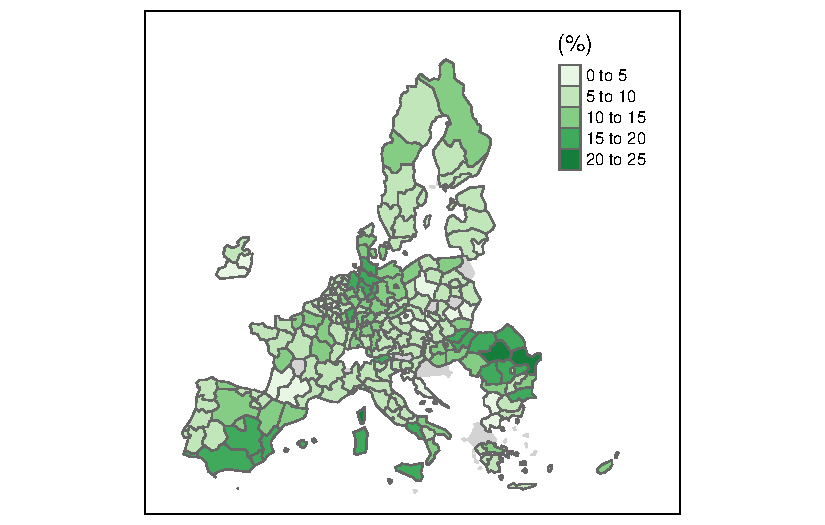
\includegraphics[width=1\textwidth,height=\textheight]{report_files/figure-pdf/mappa esl-1.pdf}

}

\caption{Early School Levers in the EU}

\end{figure}%

Research has identified several factors that contribute to early school
leaving. These factors include academic struggles, negative school
experiences, socio-economic background, and school policies such as
ability grouping. Students with lower reading levels at the start of
secondary education are particularly vulnerable to dropping out. Early
educational failures and lack of support for academic difficulties play
a significant role in this issue, as do the broader school environment
and practices that may alienate or inadequately address the needs of
struggling students.

While there are many non-quantifiable factors that influence early
school leaving, this study focuses on the causes for which we have data,
providing a quantitative analysis of the issue. By examining measurable
factors, we aim to offer a clear and evidence-based understanding of the
patterns and determinants of early school leaving in the European Union.

Given the complexity and multifaceted nature of early school leaving, it
is critical to explore the various underlying causes comprehensively.
The next section will review the scientific literature to provide a
detailed analysis of these causes, drawing on recent studies and
empirical evidence within the European Union context.

\section{Causes of Early School Leaving in Scientific
Literature}\label{causes-of-early-school-leaving-in-scientific-literature}

To best understand the causes of ESL, a multidisciplinary approach, both
theoretical and empirical (wherever possible), is needed. Therefore, we
will list all the causes of ESL, which we will then try to translate
into explanatory variables in Section 3 to study the phenomenon
quantitatively.

\subsection{Psychological and Individual
Factors}\label{psychological-and-individual-factors}

Students with low cognitive ability show a high susceptibility to ESL:
lack of achievement and demonstrated poor performance demotivate the
individual to continue with schooling (Bosoanca 2021). In fact, studies
highlight that students with lower reading levels at the onset of
second-level education are more prone to dropping out in subsequent
years. Early school leaving is often rooted in initial educational
failures and academic struggles, emphasizing the necessity for
comprehensive educational policies across all sectors (Byrne and Smyth
2010).

Yet, early school leaving is influenced not only by academic
underachievement but also by the school's response to these challenges.
Notably, some students felt neglected in academically engaged schools,
while others faced concentrated academic difficulties and misbehavior in
specific classes, frequently due to ability grouping practices (Byrne
and Smyth 2010).

\subsection{Cultural and Social
Factors}\label{cultural-and-social-factors}

The role of the family is crucial in students' school life, not only
because of the economic factor but also because of the cultural factor.
If no family member has a college degree, it is very likely that their
children will not go to college either. In addition, the children of
single parents have a high probability of being ESLs. If one member in
the family unit has already left school, the individual being considered
will have a high probability of following the same path (Bitsakos 2021).

\subsection{Economic Factors}\label{economic-factors}

The risk of students dropping out of school is highest among those who
have parents with low levels of education but only if those parents have
low incomes (Bitsakos 2021). This happens because young people are
induced to contribute to family income; this dynamic especially affects
working-class boys (Byrne and Smyth 2010). This pattern ends up in a
vicious cycle that prevents social climbing: most low-educated
individuals are more likely to get a low-income job and so on,
especially in a shrinking market.

Turning to the macro level, in fact, low-educated people not only fail
to climb out of poverty, but also fail to contribute to the growth of
the economic system in which they are immersed.

\subsection{Demographic Factors}\label{demographic-factors}

Higher dropout rates are observed among minority groups, specifically
immigrant students. For newcomer students, dropout rates are not linked
to mobility or emigration but may be related to factors like age at
immigration, language barriers, school experiences, or broader social
issues (Byrne and Smyth 2010).

Additionally, according to some research, pupils are much less likely to
drop out of school if there is more homogeneity within the structure,
both economic and ethnic (Bosoanca 2021). Moreover, according to De
Witte and Van Klaveren (2012), there are more cases of school dropouts
in rural areas than in areas with another degree of urbanization, such
as medium and large cities.

\section{The Quantitative Analysis}\label{the-quantitative-analysis}

The quantitative analysis that you will want to conduct below will be a
multiple linear regression model: the goal will be to find significant
causes of ESL among demographic and socioeconomic characteristics of the
population.

\subsection{Data Collection and
Characteristicsristics}\label{data-collection-and-characteristicsristics}

Each unit analyzed is a NUTS 2 region of the European Union; they may be
``Provincies/Provinces'' for Belgium, ``Comunididades y ciudades
autónomas'' for Spain, ``Régions'' for France, ``Länder'' for Austria,
and ``Regioni'' for Italy. NUTS 2 regions have populations ranging from
800,000 to 3 million, with a few exceptions. If no appropriately sized
administrative units exist in a member state, this level is formed by
aggregating an appropriate number of smaller and contiguous
administrative units. These units thus aggregated are called
``nonadministrative units''. The current NUTS 2021 classification came
into effect on January 1, 2021 and indicates 242 at NUTS level 2
(Gouardères 2024).

The year considered for our analysis is 2023 but since there were
missing data for certain years and regions, we went back one year at a
time until 2018 for the imputation of those data. Regions for which data
could not be imputed were excluded from the dataset.

\begin{longtable}[]{@{}ll@{}}
\caption{Excluded Regions from the Analysis}\tabularnewline
\toprule\noalign{}
Region & Country \\
\midrule\noalign{}
\endfirsthead
\toprule\noalign{}
Region & Country \\
\midrule\noalign{}
\endhead
\bottomrule\noalign{}
\endlastfoot
Burgenland & AT \\
Kärnten & AT \\
Voreio Aigaio & EL \\
Dytiki Makedonia & EL \\
Ipeiros & EL \\
Thessalia & EL \\
Ionia Nisia & EL \\
Åland & FI \\
Limousin & FR \\
Mayotte & FR \\
Kontinentalna Hrvatska & HR \\
Valle d'Aosta/Vallée d'Aoste & IT \\
Malta & MT \\
Opolskie & PL \\
Świętokrzyskie & PL \\
Podlaskie & PL \\
Região Autónoma da Madeira & PT \\
Bratislavský kraj & SK \\
\end{longtable}

All data were collected from Eurostat Database.

\subsection{Response variable}\label{response-variable}

``Early leavers are defined as individuals aged 18-24 who have completed
at most a lower secondary education and were not in further education or
training during the four weeks preceding the labour force survey (LFS)''
(Eurostat 2024b).

The measure is expressed as a percentage of the total population aged
between 18 and 24.

\begin{figure}[H]

{\centering 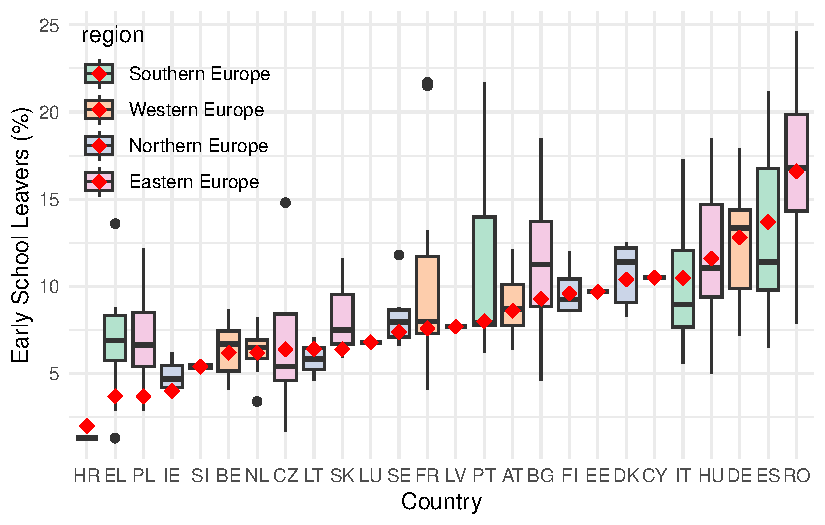
\includegraphics[width=1\textwidth,height=\textheight]{report_files/figure-pdf/boxplot esl-1.pdf}

}

\caption{Box Plot of the Response Variable per Country}

\end{figure}%

\subsection{Explanatory variables}\label{explanatory-variables}

\subsubsection{Mean Disposable Income}\label{mean-disposable-income}

``The disposable income of private households is the balance of primary
income (operating surplus/mixed income plus compensation of employees
plus property income received minus property income paid) and the
redistribution of income in cash. These transactions comprise social
contributions paid, social benefits in cash received, current taxes on
income and wealth paid, as well as other current transfers. Disposable
income does not include social transfers in kind coming from public
administrations or non-profit institutions serving households''
(Eurostat 2024a).

We took the disposable income and divided for the population, obtaining
the mean. The measure is expressed in thousands of euros.

\begin{figure}[H]

{\centering 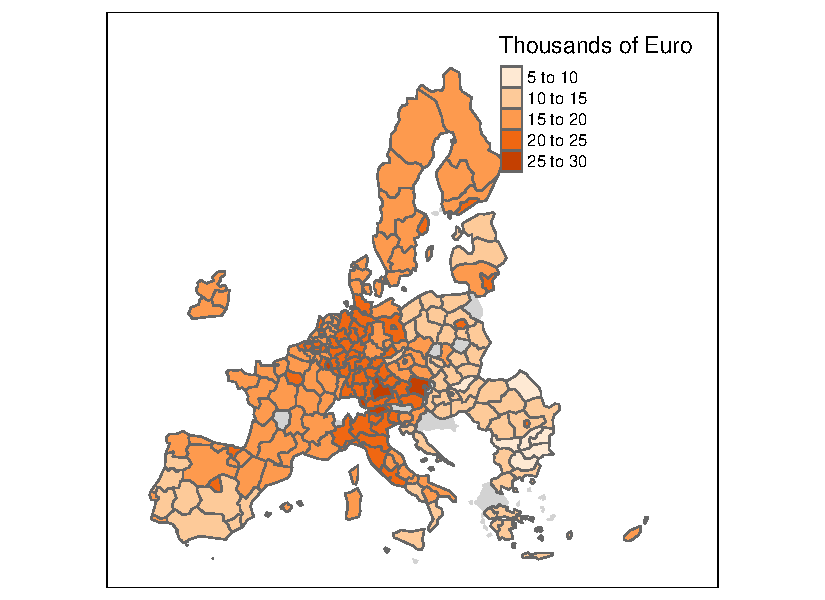
\includegraphics[width=1\textwidth,height=\textheight]{report_files/figure-pdf/mappa income-1.pdf}

}

\caption{Mean Disposable income in the EU}

\end{figure}%

\begin{figure}[H]

{\centering 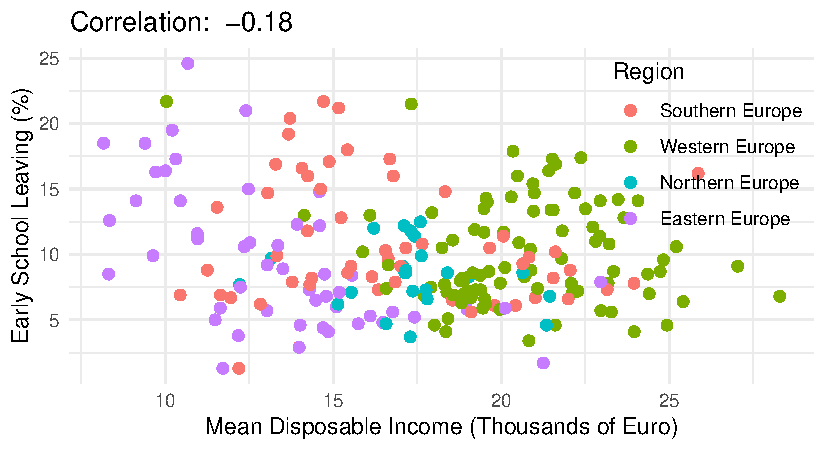
\includegraphics[width=1\textwidth,height=\textheight]{report_files/figure-pdf/scatter income-1.pdf}

}

\caption{Scatterplot of Mean Disposable Income vs Early School Leaving}

\end{figure}%

A preliminary analysis was conducted to explore the relationship between
the dependent variable ESL and the independent variable Mean Disposable
Income (MDI) using simple linear regression. Initially, a Box-Cox
transformation was employed to identify the most suitable power
transformation for the response variable ESL, with the goal of
stabilizing variance and achieving normality. This transformation is
crucial to meet the assumptions of linear regression and improve model
performance.

\begin{figure}[H]

{\centering 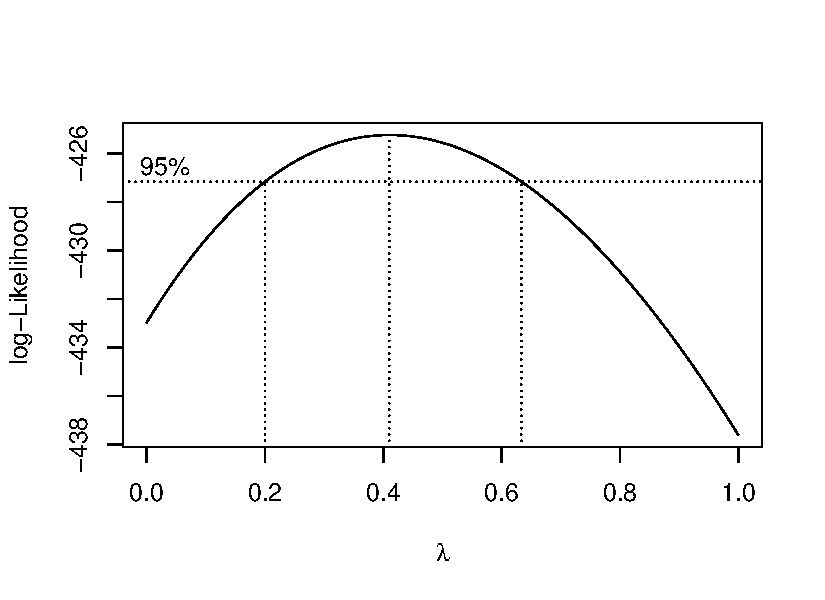
\includegraphics[width=1\textwidth,height=\textheight]{report_files/figure-pdf/box_cox_disp_inc-1.pdf}

}

\caption{Box-Plot Likelihood of Mean Disposable Income}

\end{figure}%

In order to avoid autocorrelation, we randomly selected a sample of 100
observations from the original dataset; it will be done with all the
other regression models. The selected data underwent specific
transformations: the variable ESL was transformed using a square root
transformation to stabilize variance and approximate normality.
Meanwhile, MDI was transformed using a logarithm to achieve a more
symmetric distribution. With these transformed variables, we fitted a
linear model using the sampled dataset and then, to validate the model
assumptions, several diagnostic tests were conducted. The Shapiro-Wilk
test evaluated the normality of residuals, yielding a p-value greater
than 0.05, which indicates that the residuals were approximately
normally distributed. The Breusch-Pagan test assessed the
homoscedasticity of the residuals, and its results suggested no
significant evidence of heteroscedasticity. Additionally, the
Durbin-Watson test was used to check for autocorrelation, and the
outcome indicated that there was no significant autocorrelation in the
residuals.

\begin{longtable}[]{@{}rrr@{}}
\caption{Test Results of Regression with Mean Disposable
Income}\tabularnewline
\toprule\noalign{}
Shapiro-Wilk & Breusch-Pagan.BP & Durbin-Watson \\
\midrule\noalign{}
\endfirsthead
\toprule\noalign{}
Shapiro-Wilk & Breusch-Pagan.BP & Durbin-Watson \\
\midrule\noalign{}
\endhead
\bottomrule\noalign{}
\endlastfoot
0.328904 & 0.1751287 & 0.568 \\
\end{longtable}

The results from the regression analysis reveal that the transformed
variable MDI is statistically significant at the 0.05 significance
level. However, the R-squared value of the model is 0.07, indicating
that only 7\% of the variability in ESL is explained by this model,
suggesting that there are other factors not taken into consideration.
This highlights the potential need for further investigation and
inclusion of additional predictors to improve the model's explanatory
power.

\global\setlength{\Oldarrayrulewidth}{\arrayrulewidth}

\global\setlength{\Oldtabcolsep}{\tabcolsep}

\setlength{\tabcolsep}{2pt}

\renewcommand*{\arraystretch}{1.5}



\providecommand{\ascline}[3]{\noalign{\global\arrayrulewidth #1}\arrayrulecolor[HTML]{#2}\cline{#3}}

\begin{longtable*}[c]{|p{1.01in}|p{0.88in}|p{1.29in}|p{0.75in}|p{0.75in}|p{0.40in}}



\ascline{1.5pt}{666666}{1-6}

\multicolumn{1}{>{\raggedright}m{\dimexpr 1.01in+0\tabcolsep}}{\textcolor[HTML]{000000}{\fontsize{11}{11}\selectfont{\global\setmainfont{Arial}{}}}} & \multicolumn{1}{>{\raggedleft}m{\dimexpr 0.88in+0\tabcolsep}}{\textcolor[HTML]{000000}{\fontsize{11}{11}\selectfont{\global\setmainfont{Arial}{Estimate}}}} & \multicolumn{1}{>{\raggedleft}m{\dimexpr 1.29in+0\tabcolsep}}{\textcolor[HTML]{000000}{\fontsize{11}{11}\selectfont{\global\setmainfont{Arial}{Standard\ Error}}}} & \multicolumn{1}{>{\raggedleft}m{\dimexpr 0.75in+0\tabcolsep}}{\textcolor[HTML]{000000}{\fontsize{11}{11}\selectfont{\global\setmainfont{Arial}{t\ value}}}} & \multicolumn{1}{>{\raggedleft}m{\dimexpr 0.75in+0\tabcolsep}}{\textcolor[HTML]{000000}{\fontsize{11}{11}\selectfont{\global\setmainfont{Arial}{Pr(>|t|)}}}} & \multicolumn{1}{>{\raggedright}m{\dimexpr 0.4in+0\tabcolsep}}{\textcolor[HTML]{000000}{\fontsize{11}{11}\selectfont{\global\setmainfont{Arial}{}}}} \\

\ascline{1.5pt}{666666}{1-6}\endfirsthead 

\ascline{1.5pt}{666666}{1-6}

\multicolumn{1}{>{\raggedright}m{\dimexpr 1.01in+0\tabcolsep}}{\textcolor[HTML]{000000}{\fontsize{11}{11}\selectfont{\global\setmainfont{Arial}{}}}} & \multicolumn{1}{>{\raggedleft}m{\dimexpr 0.88in+0\tabcolsep}}{\textcolor[HTML]{000000}{\fontsize{11}{11}\selectfont{\global\setmainfont{Arial}{Estimate}}}} & \multicolumn{1}{>{\raggedleft}m{\dimexpr 1.29in+0\tabcolsep}}{\textcolor[HTML]{000000}{\fontsize{11}{11}\selectfont{\global\setmainfont{Arial}{Standard\ Error}}}} & \multicolumn{1}{>{\raggedleft}m{\dimexpr 0.75in+0\tabcolsep}}{\textcolor[HTML]{000000}{\fontsize{11}{11}\selectfont{\global\setmainfont{Arial}{t\ value}}}} & \multicolumn{1}{>{\raggedleft}m{\dimexpr 0.75in+0\tabcolsep}}{\textcolor[HTML]{000000}{\fontsize{11}{11}\selectfont{\global\setmainfont{Arial}{Pr(>|t|)}}}} & \multicolumn{1}{>{\raggedright}m{\dimexpr 0.4in+0\tabcolsep}}{\textcolor[HTML]{000000}{\fontsize{11}{11}\selectfont{\global\setmainfont{Arial}{}}}} \\

\ascline{1.5pt}{666666}{1-6}\endhead



\multicolumn{1}{>{\raggedright}m{\dimexpr 1.01in+0\tabcolsep}}{\textcolor[HTML]{000000}{\fontsize{11}{11}\selectfont{\global\setmainfont{Arial}{(Intercept)}}}} & \multicolumn{1}{>{\raggedleft}m{\dimexpr 0.88in+0\tabcolsep}}{\textcolor[HTML]{000000}{\fontsize{11}{11}\selectfont{\global\setmainfont{Arial}{3.481}}}} & \multicolumn{1}{>{\raggedleft}m{\dimexpr 1.29in+0\tabcolsep}}{\textcolor[HTML]{000000}{\fontsize{11}{11}\selectfont{\global\setmainfont{Arial}{0.743}}}} & \multicolumn{1}{>{\raggedleft}m{\dimexpr 0.75in+0\tabcolsep}}{\textcolor[HTML]{000000}{\fontsize{11}{11}\selectfont{\global\setmainfont{Arial}{4.688}}}} & \multicolumn{1}{>{\raggedleft}m{\dimexpr 0.75in+0\tabcolsep}}{\textcolor[HTML]{000000}{\fontsize{11}{11}\selectfont{\global\setmainfont{Arial}{0.0000}}}} & \multicolumn{1}{>{\raggedright}m{\dimexpr 0.4in+0\tabcolsep}}{\textcolor[HTML]{000000}{\fontsize{11}{11}\selectfont{\global\setmainfont{Arial}{***}}}} \\





\multicolumn{1}{>{\raggedright}m{\dimexpr 1.01in+0\tabcolsep}}{\textcolor[HTML]{000000}{\fontsize{11}{11}\selectfont{\global\setmainfont{Arial}{z\_disp\_inc}}}} & \multicolumn{1}{>{\raggedleft}m{\dimexpr 0.88in+0\tabcolsep}}{\textcolor[HTML]{000000}{\fontsize{11}{11}\selectfont{\global\setmainfont{Arial}{-0.680}}}} & \multicolumn{1}{>{\raggedleft}m{\dimexpr 1.29in+0\tabcolsep}}{\textcolor[HTML]{000000}{\fontsize{11}{11}\selectfont{\global\setmainfont{Arial}{0.259}}}} & \multicolumn{1}{>{\raggedleft}m{\dimexpr 0.75in+0\tabcolsep}}{\textcolor[HTML]{000000}{\fontsize{11}{11}\selectfont{\global\setmainfont{Arial}{-2.622}}}} & \multicolumn{1}{>{\raggedleft}m{\dimexpr 0.75in+0\tabcolsep}}{\textcolor[HTML]{000000}{\fontsize{11}{11}\selectfont{\global\setmainfont{Arial}{0.0101}}}} & \multicolumn{1}{>{\raggedright}m{\dimexpr 0.4in+0\tabcolsep}}{\textcolor[HTML]{000000}{\fontsize{11}{11}\selectfont{\global\setmainfont{Arial}{\ \ *}}}} \\

\ascline{1.5pt}{666666}{1-6}



\multicolumn{6}{>{\raggedleft}m{\dimexpr 5.08in+10\tabcolsep}}{\textcolor[HTML]{000000}{\fontsize{11}{11}\selectfont{\global\setmainfont{Arial}{\textit{Signif.\ codes:\ 0\ <=\ '***'\ <\ 0.001\ <\ '**'\ <\ 0.01\ <\ '*'\ <\ 0.05}}}}} \\





\multicolumn{6}{>{\raggedright}m{\dimexpr 5.08in+10\tabcolsep}}{\textcolor[HTML]{000000}{\fontsize{11}{11}\selectfont{\global\setmainfont{Arial}{}}}} \\





\multicolumn{6}{>{\raggedright}m{\dimexpr 5.08in+10\tabcolsep}}{\textcolor[HTML]{000000}{\fontsize{11}{11}\selectfont{\global\setmainfont{Arial}{Residual\ standard\ error:\ 0.6457\ on\ 98\ degrees\ of\ freedom}}}} \\





\multicolumn{6}{>{\raggedright}m{\dimexpr 5.08in+10\tabcolsep}}{\textcolor[HTML]{000000}{\fontsize{11}{11}\selectfont{\global\setmainfont{Arial}{Multiple\ R-squared:\ 0.06556,\ Adjusted\ R-squared:\ 0.05603}}}} \\





\multicolumn{6}{>{\raggedright}m{\dimexpr 5.08in+10\tabcolsep}}{\textcolor[HTML]{000000}{\fontsize{11}{11}\selectfont{\global\setmainfont{Arial}{F-statistic:\ 6.876\ on\ 98\ and\ 1\ DF,\ p-value:\ 0.0101}}}} \\





\end{longtable*}



\arrayrulecolor[HTML]{000000}

\global\setlength{\arrayrulewidth}{\Oldarrayrulewidth}

\global\setlength{\tabcolsep}{\Oldtabcolsep}

\renewcommand*{\arraystretch}{1}

\subsubsection{Population Density}\label{population-density}

Since, according to some studies, most of the ESL are concentrated in
rural areas and thus outside the capital cities, we will take into
account the population density of the regions concerned.

``The ratio between the annual average population and the land area of
the region. The land area concept (excluding inland waters) should be
used wherever available; if not available then the total area, including
inland waters (area of lakes and rivers) is used'' (Eurostat 2024g).

The measure is expressed in hundreds of inhabitants per square
kilometer.

\subsubsection{Unemployment Rate}\label{unemployment-rate}

'' {[}\ldots{]} unemployment rate represents unemployed persons as a
percentage of the economically active population (i.e.~labour force or
sum of employed and unemployed). The indicator is based on the EU Labour
Force Survey. Unemployed persons comprise persons aged 15-74 who were
(all three conditions must be fulfilled simultaneously): 1. without work
during the reference week; 2. currently available for work; 3. actively
seeking work or who had found a job to start within a period of at most
three months. The employed persons are those aged 15-64, who during the
reference week did any work for pay, profit or family gain for at least
one hour, or were not at work but had a job or business from which they
were temporarily absent'' (Eurostat 2024i).

\begin{figure}[H]

{\centering 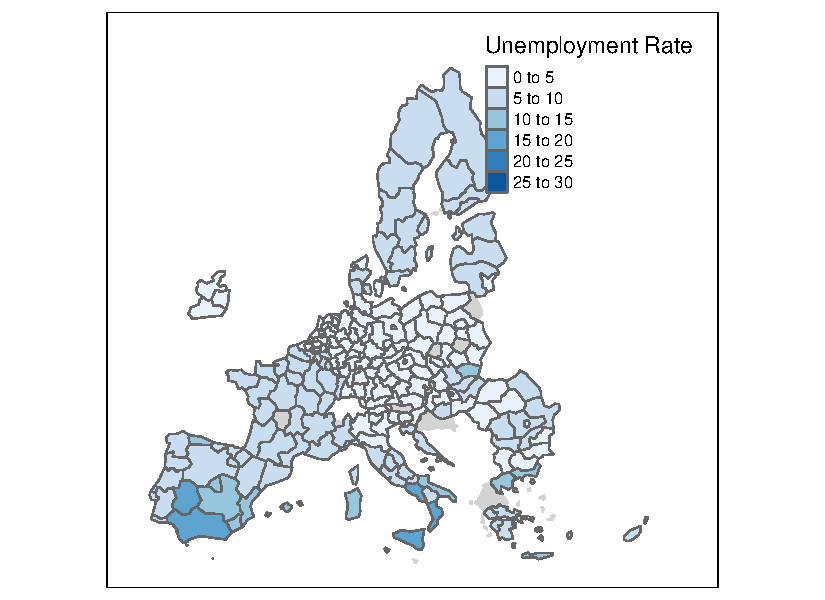
\includegraphics[width=1\textwidth,height=\textheight]{report_files/figure-pdf/mappa unemployment-1.pdf}

}

\caption{Unemployment Rate}

\end{figure}%

\begin{figure}[H]

{\centering 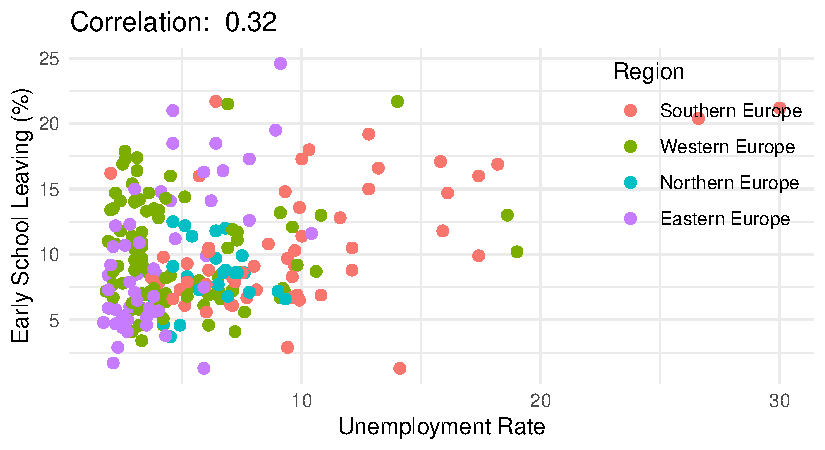
\includegraphics[width=1\textwidth,height=\textheight]{report_files/figure-pdf/scatter unemployment-1.pdf}

}

\caption{Scatterplot of Unemployment vs Early School Leaving}

\end{figure}%

The effect of Unemployment on ESL was investigated by another simple
linear regression model, which was again fitted with the square root
transformation of ESL as the dependent variable and Unemployment (there
was no need for transormation here) as the independent variable, using
the same sampled dataset.

Diagnostic tests were performed to assess the validity of the regression
model assumptions, which showed that residuals were approximately
normally distributed, no evidence of heteroscedasticity, and no
significant autocorrelation.

\begin{longtable}[]{@{}rrr@{}}
\caption{Test Results of Regression with Unemployment}\tabularnewline
\toprule\noalign{}
Shapiro-Wilk & Breusch-Pagan.BP & Durbin-Watson \\
\midrule\noalign{}
\endfirsthead
\toprule\noalign{}
Shapiro-Wilk & Breusch-Pagan.BP & Durbin-Watson \\
\midrule\noalign{}
\endhead
\bottomrule\noalign{}
\endlastfoot
0.0557342 & 0.4568521 & 0.386 \\
\end{longtable}

The regression results revealed that the predictor Unemployment is
statistically significant at the 0.01 significance level, indicating a
meaningful impact on ESL. However, similar to the previous model with
MDI, the R-squared value was relatively low (0.09), suggesting that
unemployment alone does not capture the majority of the variability in
ESL.

\global\setlength{\Oldarrayrulewidth}{\arrayrulewidth}

\global\setlength{\Oldtabcolsep}{\tabcolsep}

\setlength{\tabcolsep}{2pt}

\renewcommand*{\arraystretch}{1.5}



\providecommand{\ascline}[3]{\noalign{\global\arrayrulewidth #1}\arrayrulecolor[HTML]{#2}\cline{#3}}

\begin{longtable*}[c]{|p{1.29in}|p{0.88in}|p{1.29in}|p{0.75in}|p{0.75in}|p{0.40in}}



\ascline{1.5pt}{666666}{1-6}

\multicolumn{1}{>{\raggedright}m{\dimexpr 1.29in+0\tabcolsep}}{\textcolor[HTML]{000000}{\fontsize{11}{11}\selectfont{\global\setmainfont{Arial}{}}}} & \multicolumn{1}{>{\raggedleft}m{\dimexpr 0.88in+0\tabcolsep}}{\textcolor[HTML]{000000}{\fontsize{11}{11}\selectfont{\global\setmainfont{Arial}{Estimate}}}} & \multicolumn{1}{>{\raggedleft}m{\dimexpr 1.29in+0\tabcolsep}}{\textcolor[HTML]{000000}{\fontsize{11}{11}\selectfont{\global\setmainfont{Arial}{Standard\ Error}}}} & \multicolumn{1}{>{\raggedleft}m{\dimexpr 0.75in+0\tabcolsep}}{\textcolor[HTML]{000000}{\fontsize{11}{11}\selectfont{\global\setmainfont{Arial}{t\ value}}}} & \multicolumn{1}{>{\raggedleft}m{\dimexpr 0.75in+0\tabcolsep}}{\textcolor[HTML]{000000}{\fontsize{11}{11}\selectfont{\global\setmainfont{Arial}{Pr(>|t|)}}}} & \multicolumn{1}{>{\raggedright}m{\dimexpr 0.4in+0\tabcolsep}}{\textcolor[HTML]{000000}{\fontsize{11}{11}\selectfont{\global\setmainfont{Arial}{}}}} \\

\ascline{1.5pt}{666666}{1-6}\endfirsthead 

\ascline{1.5pt}{666666}{1-6}

\multicolumn{1}{>{\raggedright}m{\dimexpr 1.29in+0\tabcolsep}}{\textcolor[HTML]{000000}{\fontsize{11}{11}\selectfont{\global\setmainfont{Arial}{}}}} & \multicolumn{1}{>{\raggedleft}m{\dimexpr 0.88in+0\tabcolsep}}{\textcolor[HTML]{000000}{\fontsize{11}{11}\selectfont{\global\setmainfont{Arial}{Estimate}}}} & \multicolumn{1}{>{\raggedleft}m{\dimexpr 1.29in+0\tabcolsep}}{\textcolor[HTML]{000000}{\fontsize{11}{11}\selectfont{\global\setmainfont{Arial}{Standard\ Error}}}} & \multicolumn{1}{>{\raggedleft}m{\dimexpr 0.75in+0\tabcolsep}}{\textcolor[HTML]{000000}{\fontsize{11}{11}\selectfont{\global\setmainfont{Arial}{t\ value}}}} & \multicolumn{1}{>{\raggedleft}m{\dimexpr 0.75in+0\tabcolsep}}{\textcolor[HTML]{000000}{\fontsize{11}{11}\selectfont{\global\setmainfont{Arial}{Pr(>|t|)}}}} & \multicolumn{1}{>{\raggedright}m{\dimexpr 0.4in+0\tabcolsep}}{\textcolor[HTML]{000000}{\fontsize{11}{11}\selectfont{\global\setmainfont{Arial}{}}}} \\

\ascline{1.5pt}{666666}{1-6}\endhead



\multicolumn{1}{>{\raggedright}m{\dimexpr 1.29in+0\tabcolsep}}{\textcolor[HTML]{000000}{\fontsize{11}{11}\selectfont{\global\setmainfont{Arial}{(Intercept)}}}} & \multicolumn{1}{>{\raggedleft}m{\dimexpr 0.88in+0\tabcolsep}}{\textcolor[HTML]{000000}{\fontsize{11}{11}\selectfont{\global\setmainfont{Arial}{1.220}}}} & \multicolumn{1}{>{\raggedleft}m{\dimexpr 1.29in+0\tabcolsep}}{\textcolor[HTML]{000000}{\fontsize{11}{11}\selectfont{\global\setmainfont{Arial}{0.119}}}} & \multicolumn{1}{>{\raggedleft}m{\dimexpr 0.75in+0\tabcolsep}}{\textcolor[HTML]{000000}{\fontsize{11}{11}\selectfont{\global\setmainfont{Arial}{10.243}}}} & \multicolumn{1}{>{\raggedleft}m{\dimexpr 0.75in+0\tabcolsep}}{\textcolor[HTML]{000000}{\fontsize{11}{11}\selectfont{\global\setmainfont{Arial}{0.0000}}}} & \multicolumn{1}{>{\raggedright}m{\dimexpr 0.4in+0\tabcolsep}}{\textcolor[HTML]{000000}{\fontsize{11}{11}\selectfont{\global\setmainfont{Arial}{***}}}} \\





\multicolumn{1}{>{\raggedright}m{\dimexpr 1.29in+0\tabcolsep}}{\textcolor[HTML]{000000}{\fontsize{11}{11}\selectfont{\global\setmainfont{Arial}{unemployment}}}} & \multicolumn{1}{>{\raggedleft}m{\dimexpr 0.88in+0\tabcolsep}}{\textcolor[HTML]{000000}{\fontsize{11}{11}\selectfont{\global\setmainfont{Arial}{0.057}}}} & \multicolumn{1}{>{\raggedleft}m{\dimexpr 1.29in+0\tabcolsep}}{\textcolor[HTML]{000000}{\fontsize{11}{11}\selectfont{\global\setmainfont{Arial}{0.018}}}} & \multicolumn{1}{>{\raggedleft}m{\dimexpr 0.75in+0\tabcolsep}}{\textcolor[HTML]{000000}{\fontsize{11}{11}\selectfont{\global\setmainfont{Arial}{3.189}}}} & \multicolumn{1}{>{\raggedleft}m{\dimexpr 0.75in+0\tabcolsep}}{\textcolor[HTML]{000000}{\fontsize{11}{11}\selectfont{\global\setmainfont{Arial}{0.0019}}}} & \multicolumn{1}{>{\raggedright}m{\dimexpr 0.4in+0\tabcolsep}}{\textcolor[HTML]{000000}{\fontsize{11}{11}\selectfont{\global\setmainfont{Arial}{\ **}}}} \\

\ascline{1.5pt}{666666}{1-6}



\multicolumn{6}{>{\raggedleft}m{\dimexpr 5.36in+10\tabcolsep}}{\textcolor[HTML]{000000}{\fontsize{11}{11}\selectfont{\global\setmainfont{Arial}{\textit{Signif.\ codes:\ 0\ <=\ '***'\ <\ 0.001\ <\ '**'\ <\ 0.01\ <\ '*'\ <\ 0.05}}}}} \\





\multicolumn{6}{>{\raggedright}m{\dimexpr 5.36in+10\tabcolsep}}{\textcolor[HTML]{000000}{\fontsize{11}{11}\selectfont{\global\setmainfont{Arial}{}}}} \\





\multicolumn{6}{>{\raggedright}m{\dimexpr 5.36in+10\tabcolsep}}{\textcolor[HTML]{000000}{\fontsize{11}{11}\selectfont{\global\setmainfont{Arial}{Residual\ standard\ error:\ 0.6358\ on\ 98\ degrees\ of\ freedom}}}} \\





\multicolumn{6}{>{\raggedright}m{\dimexpr 5.36in+10\tabcolsep}}{\textcolor[HTML]{000000}{\fontsize{11}{11}\selectfont{\global\setmainfont{Arial}{Multiple\ R-squared:\ 0.094,\ Adjusted\ R-squared:\ 0.08475}}}} \\





\multicolumn{6}{>{\raggedright}m{\dimexpr 5.36in+10\tabcolsep}}{\textcolor[HTML]{000000}{\fontsize{11}{11}\selectfont{\global\setmainfont{Arial}{F-statistic:\ 10.17\ on\ 98\ and\ 1\ DF,\ p-value:\ 0.0019}}}} \\





\end{longtable*}



\arrayrulecolor[HTML]{000000}

\global\setlength{\arrayrulewidth}{\Oldarrayrulewidth}

\global\setlength{\tabcolsep}{\Oldtabcolsep}

\renewcommand*{\arraystretch}{1}

\subsubsection{Human Resources in Science and
Technology}\label{human-resources-in-science-and-technology}

``Human resources in science and technology as a share of the active
population in the age group 15-74 at the regional NUTS 2 level. The data
shows the active population in the age group 15-74 that is classified as
HRST (i.e.~having successfully completed an education at the third level
or being employed in science and technology) as a percentage of total
active population aged 15-74. HRST are measured mainly using the
concepts and definitions laid down in the Canberra Manual, OECD, Paris,
1995'' (Eurostat 2024d).

\begin{figure}[H]

{\centering 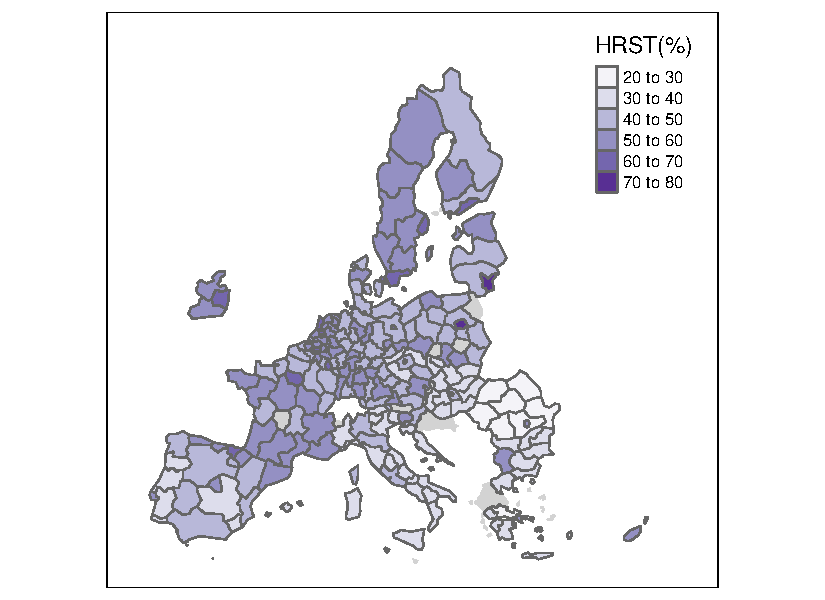
\includegraphics[width=1\textwidth,height=\textheight]{report_files/figure-pdf/mappa HRST-1.pdf}

}

\caption{Human Resources in Science and Technology(\%)}

\end{figure}%

\begin{figure}[H]

{\centering 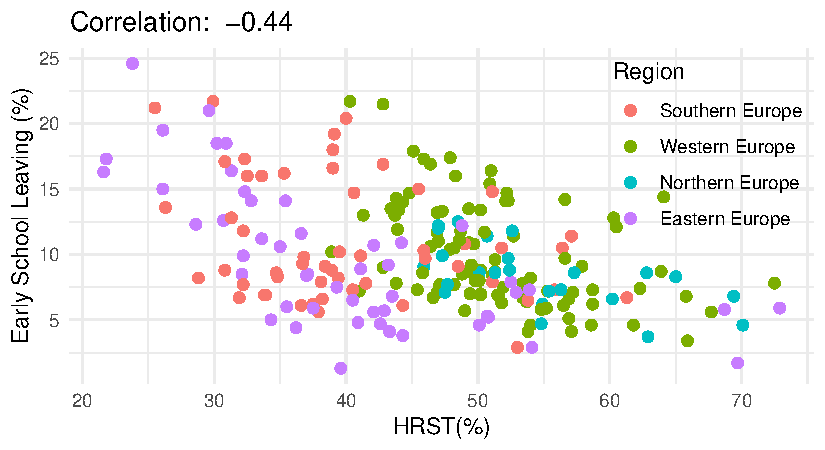
\includegraphics[width=1\textwidth,height=\textheight]{report_files/figure-pdf/scatter HRST-1.pdf}

}

\caption{Scatterplot of Human Resources in Science and Technology(\%) vs
Early School Leaving}

\end{figure}%

Further analysis was conducted to examine the effect of Human Resources
in Science and Technology (HRST) on the same transormation of ESL, using
the same sampled dataset.

Once again, diagnostic tests were performed to assess model assumptions.
The Shapiro-Wilk test indicated normality of residuals, the
Breusch-Pagan test showed homoscedasticity, and the Durbin-Watson test
confirmed no significant autocorrelation.

\begin{longtable}[]{@{}rrr@{}}
\caption{Test Results of Regression with Human Resources in Science and
Technology}\tabularnewline
\toprule\noalign{}
Shapiro-Wilk & Breusch-Pagan.BP & Durbin-Watson \\
\midrule\noalign{}
\endfirsthead
\toprule\noalign{}
Shapiro-Wilk & Breusch-Pagan.BP & Durbin-Watson \\
\midrule\noalign{}
\endhead
\bottomrule\noalign{}
\endlastfoot
0.8217867 & 0.1218665 & 0.358 \\
\end{longtable}

The regression results demonstrated that HRST is statistically
significant at the 0.001 level, suggesting that the percentage of HRST
has a significant effect on ESL proficiency. This time, unlike the
previous analyses, the R-squared value was higher (0.25), a substantial
improvement.

\global\setlength{\Oldarrayrulewidth}{\arrayrulewidth}

\global\setlength{\Oldtabcolsep}{\tabcolsep}

\setlength{\tabcolsep}{2pt}

\renewcommand*{\arraystretch}{1.5}



\providecommand{\ascline}[3]{\noalign{\global\arrayrulewidth #1}\arrayrulecolor[HTML]{#2}\cline{#3}}

\begin{longtable*}[c]{|p{0.98in}|p{0.88in}|p{1.29in}|p{0.75in}|p{0.75in}|p{0.40in}}



\ascline{1.5pt}{666666}{1-6}

\multicolumn{1}{>{\raggedright}m{\dimexpr 0.98in+0\tabcolsep}}{\textcolor[HTML]{000000}{\fontsize{11}{11}\selectfont{\global\setmainfont{Arial}{}}}} & \multicolumn{1}{>{\raggedleft}m{\dimexpr 0.88in+0\tabcolsep}}{\textcolor[HTML]{000000}{\fontsize{11}{11}\selectfont{\global\setmainfont{Arial}{Estimate}}}} & \multicolumn{1}{>{\raggedleft}m{\dimexpr 1.29in+0\tabcolsep}}{\textcolor[HTML]{000000}{\fontsize{11}{11}\selectfont{\global\setmainfont{Arial}{Standard\ Error}}}} & \multicolumn{1}{>{\raggedleft}m{\dimexpr 0.75in+0\tabcolsep}}{\textcolor[HTML]{000000}{\fontsize{11}{11}\selectfont{\global\setmainfont{Arial}{t\ value}}}} & \multicolumn{1}{>{\raggedleft}m{\dimexpr 0.75in+0\tabcolsep}}{\textcolor[HTML]{000000}{\fontsize{11}{11}\selectfont{\global\setmainfont{Arial}{Pr(>|t|)}}}} & \multicolumn{1}{>{\raggedright}m{\dimexpr 0.4in+0\tabcolsep}}{\textcolor[HTML]{000000}{\fontsize{11}{11}\selectfont{\global\setmainfont{Arial}{}}}} \\

\ascline{1.5pt}{666666}{1-6}\endfirsthead 

\ascline{1.5pt}{666666}{1-6}

\multicolumn{1}{>{\raggedright}m{\dimexpr 0.98in+0\tabcolsep}}{\textcolor[HTML]{000000}{\fontsize{11}{11}\selectfont{\global\setmainfont{Arial}{}}}} & \multicolumn{1}{>{\raggedleft}m{\dimexpr 0.88in+0\tabcolsep}}{\textcolor[HTML]{000000}{\fontsize{11}{11}\selectfont{\global\setmainfont{Arial}{Estimate}}}} & \multicolumn{1}{>{\raggedleft}m{\dimexpr 1.29in+0\tabcolsep}}{\textcolor[HTML]{000000}{\fontsize{11}{11}\selectfont{\global\setmainfont{Arial}{Standard\ Error}}}} & \multicolumn{1}{>{\raggedleft}m{\dimexpr 0.75in+0\tabcolsep}}{\textcolor[HTML]{000000}{\fontsize{11}{11}\selectfont{\global\setmainfont{Arial}{t\ value}}}} & \multicolumn{1}{>{\raggedleft}m{\dimexpr 0.75in+0\tabcolsep}}{\textcolor[HTML]{000000}{\fontsize{11}{11}\selectfont{\global\setmainfont{Arial}{Pr(>|t|)}}}} & \multicolumn{1}{>{\raggedright}m{\dimexpr 0.4in+0\tabcolsep}}{\textcolor[HTML]{000000}{\fontsize{11}{11}\selectfont{\global\setmainfont{Arial}{}}}} \\

\ascline{1.5pt}{666666}{1-6}\endhead



\multicolumn{1}{>{\raggedright}m{\dimexpr 0.98in+0\tabcolsep}}{\textcolor[HTML]{000000}{\fontsize{11}{11}\selectfont{\global\setmainfont{Arial}{(Intercept)}}}} & \multicolumn{1}{>{\raggedleft}m{\dimexpr 0.88in+0\tabcolsep}}{\textcolor[HTML]{000000}{\fontsize{11}{11}\selectfont{\global\setmainfont{Arial}{2.978}}}} & \multicolumn{1}{>{\raggedleft}m{\dimexpr 1.29in+0\tabcolsep}}{\textcolor[HTML]{000000}{\fontsize{11}{11}\selectfont{\global\setmainfont{Arial}{0.261}}}} & \multicolumn{1}{>{\raggedleft}m{\dimexpr 0.75in+0\tabcolsep}}{\textcolor[HTML]{000000}{\fontsize{11}{11}\selectfont{\global\setmainfont{Arial}{11.408}}}} & \multicolumn{1}{>{\raggedleft}m{\dimexpr 0.75in+0\tabcolsep}}{\textcolor[HTML]{000000}{\fontsize{11}{11}\selectfont{\global\setmainfont{Arial}{0.0000}}}} & \multicolumn{1}{>{\raggedright}m{\dimexpr 0.4in+0\tabcolsep}}{\textcolor[HTML]{000000}{\fontsize{11}{11}\selectfont{\global\setmainfont{Arial}{***}}}} \\





\multicolumn{1}{>{\raggedright}m{\dimexpr 0.98in+0\tabcolsep}}{\textcolor[HTML]{000000}{\fontsize{11}{11}\selectfont{\global\setmainfont{Arial}{HRST}}}} & \multicolumn{1}{>{\raggedleft}m{\dimexpr 0.88in+0\tabcolsep}}{\textcolor[HTML]{000000}{\fontsize{11}{11}\selectfont{\global\setmainfont{Arial}{-0.031}}}} & \multicolumn{1}{>{\raggedleft}m{\dimexpr 1.29in+0\tabcolsep}}{\textcolor[HTML]{000000}{\fontsize{11}{11}\selectfont{\global\setmainfont{Arial}{0.005}}}} & \multicolumn{1}{>{\raggedleft}m{\dimexpr 0.75in+0\tabcolsep}}{\textcolor[HTML]{000000}{\fontsize{11}{11}\selectfont{\global\setmainfont{Arial}{-5.645}}}} & \multicolumn{1}{>{\raggedleft}m{\dimexpr 0.75in+0\tabcolsep}}{\textcolor[HTML]{000000}{\fontsize{11}{11}\selectfont{\global\setmainfont{Arial}{0.0000}}}} & \multicolumn{1}{>{\raggedright}m{\dimexpr 0.4in+0\tabcolsep}}{\textcolor[HTML]{000000}{\fontsize{11}{11}\selectfont{\global\setmainfont{Arial}{***}}}} \\

\ascline{1.5pt}{666666}{1-6}



\multicolumn{6}{>{\raggedleft}m{\dimexpr 5.05in+10\tabcolsep}}{\textcolor[HTML]{000000}{\fontsize{11}{11}\selectfont{\global\setmainfont{Arial}{\textit{Signif.\ codes:\ 0\ <=\ '***'\ <\ 0.001\ <\ '**'\ <\ 0.01\ <\ '*'\ <\ 0.05}}}}} \\





\multicolumn{6}{>{\raggedright}m{\dimexpr 5.05in+10\tabcolsep}}{\textcolor[HTML]{000000}{\fontsize{11}{11}\selectfont{\global\setmainfont{Arial}{}}}} \\





\multicolumn{6}{>{\raggedright}m{\dimexpr 5.05in+10\tabcolsep}}{\textcolor[HTML]{000000}{\fontsize{11}{11}\selectfont{\global\setmainfont{Arial}{Residual\ standard\ error:\ 0.5803\ on\ 98\ degrees\ of\ freedom}}}} \\





\multicolumn{6}{>{\raggedright}m{\dimexpr 5.05in+10\tabcolsep}}{\textcolor[HTML]{000000}{\fontsize{11}{11}\selectfont{\global\setmainfont{Arial}{Multiple\ R-squared:\ 0.2454,\ Adjusted\ R-squared:\ 0.2377}}}} \\





\multicolumn{6}{>{\raggedright}m{\dimexpr 5.05in+10\tabcolsep}}{\textcolor[HTML]{000000}{\fontsize{11}{11}\selectfont{\global\setmainfont{Arial}{F-statistic:\ 31.86\ on\ 98\ and\ 1\ DF,\ p-value:\ 0.0000}}}} \\





\end{longtable*}



\arrayrulecolor[HTML]{000000}

\global\setlength{\arrayrulewidth}{\Oldarrayrulewidth}

\global\setlength{\tabcolsep}{\Oldtabcolsep}

\renewcommand*{\arraystretch}{1}

\subsubsection{Over-25s with at most Lower Secondary
Education}\label{over-25s-with-at-most-lower-secondary-education}

Since the educational attainment of parents and people in the context
are very important for their influence on the pupil, we include the
variable of the percentage of over-25s with at most lower secondary
education (amLSE).

\begin{figure}[H]

{\centering 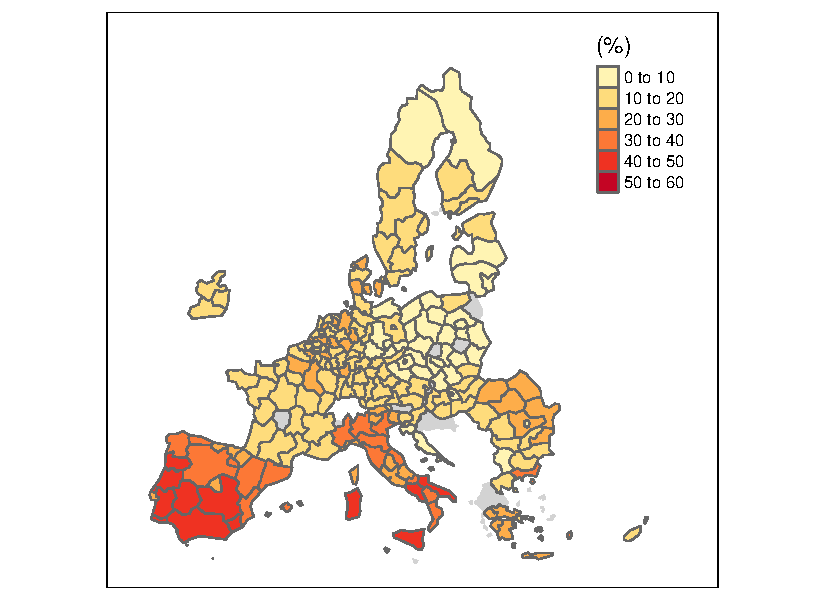
\includegraphics[width=1\textwidth,height=\textheight]{report_files/figure-pdf/mappa amLSE-1.pdf}

}

\caption{Over-25s with at most Lower Secondary Education(\%)}

\end{figure}%

\begin{figure}[H]

{\centering 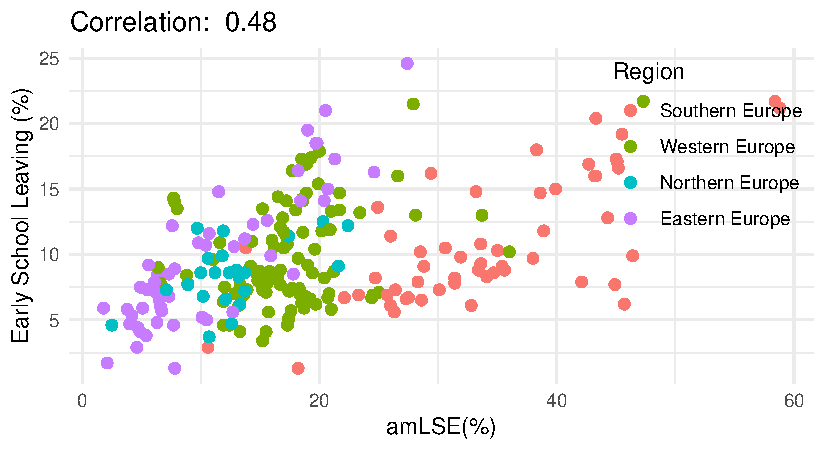
\includegraphics[width=1\textwidth,height=\textheight]{report_files/figure-pdf/scatter amLSE-1.pdf}

}

\caption{Scatterplot of Over-25s with at most Lower Secondary Education
vs Early School Leaving}

\end{figure}%

The regression model performed with amLSE as indipendent variable is
statistically significant at the 0.001 level. The R-squared value for
amLSE was 0.24, indicating that it explains 24\% of the variability in
ESL. This also demonstrates a stronger explanatory power compared to MDI
and Unemployment.

\global\setlength{\Oldarrayrulewidth}{\arrayrulewidth}

\global\setlength{\Oldtabcolsep}{\tabcolsep}

\setlength{\tabcolsep}{2pt}

\renewcommand*{\arraystretch}{1.5}



\providecommand{\ascline}[3]{\noalign{\global\arrayrulewidth #1}\arrayrulecolor[HTML]{#2}\cline{#3}}

\begin{longtable*}[c]{|p{0.98in}|p{0.88in}|p{1.29in}|p{0.75in}|p{0.75in}|p{0.40in}}



\ascline{1.5pt}{666666}{1-6}

\multicolumn{1}{>{\raggedright}m{\dimexpr 0.98in+0\tabcolsep}}{\textcolor[HTML]{000000}{\fontsize{11}{11}\selectfont{\global\setmainfont{Arial}{}}}} & \multicolumn{1}{>{\raggedleft}m{\dimexpr 0.88in+0\tabcolsep}}{\textcolor[HTML]{000000}{\fontsize{11}{11}\selectfont{\global\setmainfont{Arial}{Estimate}}}} & \multicolumn{1}{>{\raggedleft}m{\dimexpr 1.29in+0\tabcolsep}}{\textcolor[HTML]{000000}{\fontsize{11}{11}\selectfont{\global\setmainfont{Arial}{Standard\ Error}}}} & \multicolumn{1}{>{\raggedleft}m{\dimexpr 0.75in+0\tabcolsep}}{\textcolor[HTML]{000000}{\fontsize{11}{11}\selectfont{\global\setmainfont{Arial}{t\ value}}}} & \multicolumn{1}{>{\raggedleft}m{\dimexpr 0.75in+0\tabcolsep}}{\textcolor[HTML]{000000}{\fontsize{11}{11}\selectfont{\global\setmainfont{Arial}{Pr(>|t|)}}}} & \multicolumn{1}{>{\raggedright}m{\dimexpr 0.4in+0\tabcolsep}}{\textcolor[HTML]{000000}{\fontsize{11}{11}\selectfont{\global\setmainfont{Arial}{}}}} \\

\ascline{1.5pt}{666666}{1-6}\endfirsthead 

\ascline{1.5pt}{666666}{1-6}

\multicolumn{1}{>{\raggedright}m{\dimexpr 0.98in+0\tabcolsep}}{\textcolor[HTML]{000000}{\fontsize{11}{11}\selectfont{\global\setmainfont{Arial}{}}}} & \multicolumn{1}{>{\raggedleft}m{\dimexpr 0.88in+0\tabcolsep}}{\textcolor[HTML]{000000}{\fontsize{11}{11}\selectfont{\global\setmainfont{Arial}{Estimate}}}} & \multicolumn{1}{>{\raggedleft}m{\dimexpr 1.29in+0\tabcolsep}}{\textcolor[HTML]{000000}{\fontsize{11}{11}\selectfont{\global\setmainfont{Arial}{Standard\ Error}}}} & \multicolumn{1}{>{\raggedleft}m{\dimexpr 0.75in+0\tabcolsep}}{\textcolor[HTML]{000000}{\fontsize{11}{11}\selectfont{\global\setmainfont{Arial}{t\ value}}}} & \multicolumn{1}{>{\raggedleft}m{\dimexpr 0.75in+0\tabcolsep}}{\textcolor[HTML]{000000}{\fontsize{11}{11}\selectfont{\global\setmainfont{Arial}{Pr(>|t|)}}}} & \multicolumn{1}{>{\raggedright}m{\dimexpr 0.4in+0\tabcolsep}}{\textcolor[HTML]{000000}{\fontsize{11}{11}\selectfont{\global\setmainfont{Arial}{}}}} \\

\ascline{1.5pt}{666666}{1-6}\endhead



\multicolumn{1}{>{\raggedright}m{\dimexpr 0.98in+0\tabcolsep}}{\textcolor[HTML]{000000}{\fontsize{11}{11}\selectfont{\global\setmainfont{Arial}{(Intercept)}}}} & \multicolumn{1}{>{\raggedleft}m{\dimexpr 0.88in+0\tabcolsep}}{\textcolor[HTML]{000000}{\fontsize{11}{11}\selectfont{\global\setmainfont{Arial}{0.973}}}} & \multicolumn{1}{>{\raggedleft}m{\dimexpr 1.29in+0\tabcolsep}}{\textcolor[HTML]{000000}{\fontsize{11}{11}\selectfont{\global\setmainfont{Arial}{0.118}}}} & \multicolumn{1}{>{\raggedleft}m{\dimexpr 0.75in+0\tabcolsep}}{\textcolor[HTML]{000000}{\fontsize{11}{11}\selectfont{\global\setmainfont{Arial}{8.236}}}} & \multicolumn{1}{>{\raggedleft}m{\dimexpr 0.75in+0\tabcolsep}}{\textcolor[HTML]{000000}{\fontsize{11}{11}\selectfont{\global\setmainfont{Arial}{0.0000}}}} & \multicolumn{1}{>{\raggedright}m{\dimexpr 0.4in+0\tabcolsep}}{\textcolor[HTML]{000000}{\fontsize{11}{11}\selectfont{\global\setmainfont{Arial}{***}}}} \\





\multicolumn{1}{>{\raggedright}m{\dimexpr 0.98in+0\tabcolsep}}{\textcolor[HTML]{000000}{\fontsize{11}{11}\selectfont{\global\setmainfont{Arial}{amLSE}}}} & \multicolumn{1}{>{\raggedleft}m{\dimexpr 0.88in+0\tabcolsep}}{\textcolor[HTML]{000000}{\fontsize{11}{11}\selectfont{\global\setmainfont{Arial}{0.030}}}} & \multicolumn{1}{>{\raggedleft}m{\dimexpr 1.29in+0\tabcolsep}}{\textcolor[HTML]{000000}{\fontsize{11}{11}\selectfont{\global\setmainfont{Arial}{0.005}}}} & \multicolumn{1}{>{\raggedleft}m{\dimexpr 0.75in+0\tabcolsep}}{\textcolor[HTML]{000000}{\fontsize{11}{11}\selectfont{\global\setmainfont{Arial}{5.525}}}} & \multicolumn{1}{>{\raggedleft}m{\dimexpr 0.75in+0\tabcolsep}}{\textcolor[HTML]{000000}{\fontsize{11}{11}\selectfont{\global\setmainfont{Arial}{0.0000}}}} & \multicolumn{1}{>{\raggedright}m{\dimexpr 0.4in+0\tabcolsep}}{\textcolor[HTML]{000000}{\fontsize{11}{11}\selectfont{\global\setmainfont{Arial}{***}}}} \\

\ascline{1.5pt}{666666}{1-6}



\multicolumn{6}{>{\raggedleft}m{\dimexpr 5.05in+10\tabcolsep}}{\textcolor[HTML]{000000}{\fontsize{11}{11}\selectfont{\global\setmainfont{Arial}{\textit{Signif.\ codes:\ 0\ <=\ '***'\ <\ 0.001\ <\ '**'\ <\ 0.01\ <\ '*'\ <\ 0.05}}}}} \\





\multicolumn{6}{>{\raggedright}m{\dimexpr 5.05in+10\tabcolsep}}{\textcolor[HTML]{000000}{\fontsize{11}{11}\selectfont{\global\setmainfont{Arial}{}}}} \\





\multicolumn{6}{>{\raggedright}m{\dimexpr 5.05in+10\tabcolsep}}{\textcolor[HTML]{000000}{\fontsize{11}{11}\selectfont{\global\setmainfont{Arial}{Residual\ standard\ error:\ 0.5833\ on\ 98\ degrees\ of\ freedom}}}} \\





\multicolumn{6}{>{\raggedright}m{\dimexpr 5.05in+10\tabcolsep}}{\textcolor[HTML]{000000}{\fontsize{11}{11}\selectfont{\global\setmainfont{Arial}{Multiple\ R-squared:\ 0.2375,\ Adjusted\ R-squared:\ 0.2297}}}} \\





\multicolumn{6}{>{\raggedright}m{\dimexpr 5.05in+10\tabcolsep}}{\textcolor[HTML]{000000}{\fontsize{11}{11}\selectfont{\global\setmainfont{Arial}{F-statistic:\ 30.53\ on\ 98\ and\ 1\ DF,\ p-value:\ 0.0000}}}} \\





\end{longtable*}



\arrayrulecolor[HTML]{000000}

\global\setlength{\arrayrulewidth}{\Oldarrayrulewidth}

\global\setlength{\tabcolsep}{\Oldtabcolsep}

\renewcommand*{\arraystretch}{1}

\subsubsection{Tourism}\label{tourism}

We created an indicator dividing the nights spent in a tourist
accommodation by the population.

``A night spent is each night a guest/tourist (resident or non-resident)
actually spends (sleeps or stays) or is registered (his/her physical
presence there being unnecessary) in a tourist accommodation
establishment'' (Eurostat 2024e).

The effect of tourism on ESL was assessed by a linear regression model
that showed no statistical significance, with a p-value well above the
0.05 threshold. This indicates that tourism does not have a meaningful
impact on z\_esl in this model. The R-squared value was also low,
further confirming that tourism does not explain a substantial portion
of the variability in ESL proficiency.

\global\setlength{\Oldarrayrulewidth}{\arrayrulewidth}

\global\setlength{\Oldtabcolsep}{\tabcolsep}

\setlength{\tabcolsep}{2pt}

\renewcommand*{\arraystretch}{1.5}



\providecommand{\ascline}[3]{\noalign{\global\arrayrulewidth #1}\arrayrulecolor[HTML]{#2}\cline{#3}}

\begin{longtable*}[c]{|p{0.98in}|p{0.88in}|p{1.29in}|p{0.75in}|p{0.75in}|p{0.40in}}



\ascline{1.5pt}{666666}{1-6}

\multicolumn{1}{>{\raggedright}m{\dimexpr 0.98in+0\tabcolsep}}{\textcolor[HTML]{000000}{\fontsize{11}{11}\selectfont{\global\setmainfont{Arial}{}}}} & \multicolumn{1}{>{\raggedleft}m{\dimexpr 0.88in+0\tabcolsep}}{\textcolor[HTML]{000000}{\fontsize{11}{11}\selectfont{\global\setmainfont{Arial}{Estimate}}}} & \multicolumn{1}{>{\raggedleft}m{\dimexpr 1.29in+0\tabcolsep}}{\textcolor[HTML]{000000}{\fontsize{11}{11}\selectfont{\global\setmainfont{Arial}{Standard\ Error}}}} & \multicolumn{1}{>{\raggedleft}m{\dimexpr 0.75in+0\tabcolsep}}{\textcolor[HTML]{000000}{\fontsize{11}{11}\selectfont{\global\setmainfont{Arial}{t\ value}}}} & \multicolumn{1}{>{\raggedleft}m{\dimexpr 0.75in+0\tabcolsep}}{\textcolor[HTML]{000000}{\fontsize{11}{11}\selectfont{\global\setmainfont{Arial}{Pr(>|t|)}}}} & \multicolumn{1}{>{\raggedright}m{\dimexpr 0.4in+0\tabcolsep}}{\textcolor[HTML]{000000}{\fontsize{11}{11}\selectfont{\global\setmainfont{Arial}{}}}} \\

\ascline{1.5pt}{666666}{1-6}\endfirsthead 

\ascline{1.5pt}{666666}{1-6}

\multicolumn{1}{>{\raggedright}m{\dimexpr 0.98in+0\tabcolsep}}{\textcolor[HTML]{000000}{\fontsize{11}{11}\selectfont{\global\setmainfont{Arial}{}}}} & \multicolumn{1}{>{\raggedleft}m{\dimexpr 0.88in+0\tabcolsep}}{\textcolor[HTML]{000000}{\fontsize{11}{11}\selectfont{\global\setmainfont{Arial}{Estimate}}}} & \multicolumn{1}{>{\raggedleft}m{\dimexpr 1.29in+0\tabcolsep}}{\textcolor[HTML]{000000}{\fontsize{11}{11}\selectfont{\global\setmainfont{Arial}{Standard\ Error}}}} & \multicolumn{1}{>{\raggedleft}m{\dimexpr 0.75in+0\tabcolsep}}{\textcolor[HTML]{000000}{\fontsize{11}{11}\selectfont{\global\setmainfont{Arial}{t\ value}}}} & \multicolumn{1}{>{\raggedleft}m{\dimexpr 0.75in+0\tabcolsep}}{\textcolor[HTML]{000000}{\fontsize{11}{11}\selectfont{\global\setmainfont{Arial}{Pr(>|t|)}}}} & \multicolumn{1}{>{\raggedright}m{\dimexpr 0.4in+0\tabcolsep}}{\textcolor[HTML]{000000}{\fontsize{11}{11}\selectfont{\global\setmainfont{Arial}{}}}} \\

\ascline{1.5pt}{666666}{1-6}\endhead



\multicolumn{1}{>{\raggedright}m{\dimexpr 0.98in+0\tabcolsep}}{\textcolor[HTML]{000000}{\fontsize{11}{11}\selectfont{\global\setmainfont{Arial}{(Intercept)}}}} & \multicolumn{1}{>{\raggedleft}m{\dimexpr 0.88in+0\tabcolsep}}{\textcolor[HTML]{000000}{\fontsize{11}{11}\selectfont{\global\setmainfont{Arial}{1.498}}}} & \multicolumn{1}{>{\raggedleft}m{\dimexpr 1.29in+0\tabcolsep}}{\textcolor[HTML]{000000}{\fontsize{11}{11}\selectfont{\global\setmainfont{Arial}{0.078}}}} & \multicolumn{1}{>{\raggedleft}m{\dimexpr 0.75in+0\tabcolsep}}{\textcolor[HTML]{000000}{\fontsize{11}{11}\selectfont{\global\setmainfont{Arial}{19.141}}}} & \multicolumn{1}{>{\raggedleft}m{\dimexpr 0.75in+0\tabcolsep}}{\textcolor[HTML]{000000}{\fontsize{11}{11}\selectfont{\global\setmainfont{Arial}{0.0000}}}} & \multicolumn{1}{>{\raggedright}m{\dimexpr 0.4in+0\tabcolsep}}{\textcolor[HTML]{000000}{\fontsize{11}{11}\selectfont{\global\setmainfont{Arial}{***}}}} \\





\multicolumn{1}{>{\raggedright}m{\dimexpr 0.98in+0\tabcolsep}}{\textcolor[HTML]{000000}{\fontsize{11}{11}\selectfont{\global\setmainfont{Arial}{tourism}}}} & \multicolumn{1}{>{\raggedleft}m{\dimexpr 0.88in+0\tabcolsep}}{\textcolor[HTML]{000000}{\fontsize{11}{11}\selectfont{\global\setmainfont{Arial}{0.005}}}} & \multicolumn{1}{>{\raggedleft}m{\dimexpr 1.29in+0\tabcolsep}}{\textcolor[HTML]{000000}{\fontsize{11}{11}\selectfont{\global\setmainfont{Arial}{0.005}}}} & \multicolumn{1}{>{\raggedleft}m{\dimexpr 0.75in+0\tabcolsep}}{\textcolor[HTML]{000000}{\fontsize{11}{11}\selectfont{\global\setmainfont{Arial}{1.044}}}} & \multicolumn{1}{>{\raggedleft}m{\dimexpr 0.75in+0\tabcolsep}}{\textcolor[HTML]{000000}{\fontsize{11}{11}\selectfont{\global\setmainfont{Arial}{0.2990}}}} & \multicolumn{1}{>{\raggedright}m{\dimexpr 0.4in+0\tabcolsep}}{\textcolor[HTML]{000000}{\fontsize{11}{11}\selectfont{\global\setmainfont{Arial}{\ \ \ }}}} \\

\ascline{1.5pt}{666666}{1-6}



\multicolumn{6}{>{\raggedleft}m{\dimexpr 5.05in+10\tabcolsep}}{\textcolor[HTML]{000000}{\fontsize{11}{11}\selectfont{\global\setmainfont{Arial}{\textit{Signif.\ codes:\ 0\ <=\ '***'\ <\ 0.001\ <\ '**'\ <\ 0.01\ <\ '*'\ <\ 0.05}}}}} \\





\multicolumn{6}{>{\raggedright}m{\dimexpr 5.05in+10\tabcolsep}}{\textcolor[HTML]{000000}{\fontsize{11}{11}\selectfont{\global\setmainfont{Arial}{}}}} \\





\multicolumn{6}{>{\raggedright}m{\dimexpr 5.05in+10\tabcolsep}}{\textcolor[HTML]{000000}{\fontsize{11}{11}\selectfont{\global\setmainfont{Arial}{Residual\ standard\ error:\ 0.6643\ on\ 98\ degrees\ of\ freedom}}}} \\





\multicolumn{6}{>{\raggedright}m{\dimexpr 5.05in+10\tabcolsep}}{\textcolor[HTML]{000000}{\fontsize{11}{11}\selectfont{\global\setmainfont{Arial}{Multiple\ R-squared:\ 0.011,\ Adjusted\ R-squared:\ 0.0009117}}}} \\





\multicolumn{6}{>{\raggedright}m{\dimexpr 5.05in+10\tabcolsep}}{\textcolor[HTML]{000000}{\fontsize{11}{11}\selectfont{\global\setmainfont{Arial}{F-statistic:\ 1.09\ on\ 98\ and\ 1\ DF,\ p-value:\ 0.2990}}}} \\





\end{longtable*}



\arrayrulecolor[HTML]{000000}

\global\setlength{\arrayrulewidth}{\Oldarrayrulewidth}

\global\setlength{\tabcolsep}{\Oldtabcolsep}

\renewcommand*{\arraystretch}{1}

\subsubsection{Weeks of holiday from
School}\label{weeks-of-holiday-from-school}

The first dummy we used in the model concerns the weeks the student is
away from school. The cut point we took is 10 weeks away from school,
through the entire school-year.

\begin{figure}[H]

{\centering 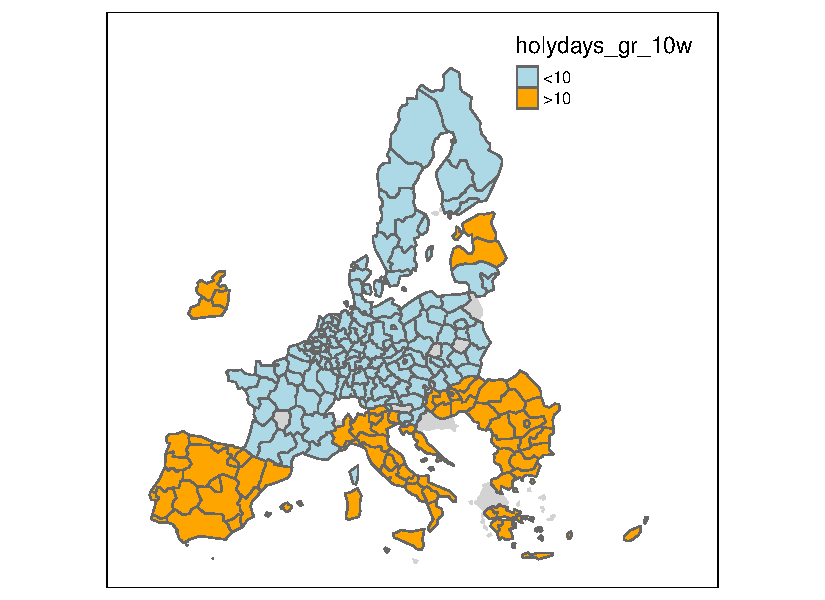
\includegraphics[width=1\textwidth,height=\textheight]{report_files/figure-pdf/mappa holydays_gr_10w-1.pdf}

}

\caption{Countries where Weeks of holiday from School are more than 10}

\end{figure}%

The regression model revealed that Weeks of holiday from School are
statistically significant at the 0.01 level, indicating that the
presence of holidays has a meaningful impact on the transformation of
the variable ESL. However, the model's R-squared value was 0.07, which
shows that it explains only 7\% of the variability in ESL.

\global\setlength{\Oldarrayrulewidth}{\arrayrulewidth}

\global\setlength{\Oldtabcolsep}{\tabcolsep}

\setlength{\tabcolsep}{2pt}

\renewcommand*{\arraystretch}{1.5}



\providecommand{\ascline}[3]{\noalign{\global\arrayrulewidth #1}\arrayrulecolor[HTML]{#2}\cline{#3}}

\begin{longtable*}[c]{|p{1.56in}|p{0.88in}|p{1.29in}|p{0.75in}|p{0.75in}|p{0.40in}}



\ascline{1.5pt}{666666}{1-6}

\multicolumn{1}{>{\raggedright}m{\dimexpr 1.56in+0\tabcolsep}}{\textcolor[HTML]{000000}{\fontsize{11}{11}\selectfont{\global\setmainfont{Arial}{}}}} & \multicolumn{1}{>{\raggedleft}m{\dimexpr 0.88in+0\tabcolsep}}{\textcolor[HTML]{000000}{\fontsize{11}{11}\selectfont{\global\setmainfont{Arial}{Estimate}}}} & \multicolumn{1}{>{\raggedleft}m{\dimexpr 1.29in+0\tabcolsep}}{\textcolor[HTML]{000000}{\fontsize{11}{11}\selectfont{\global\setmainfont{Arial}{Standard\ Error}}}} & \multicolumn{1}{>{\raggedleft}m{\dimexpr 0.75in+0\tabcolsep}}{\textcolor[HTML]{000000}{\fontsize{11}{11}\selectfont{\global\setmainfont{Arial}{t\ value}}}} & \multicolumn{1}{>{\raggedleft}m{\dimexpr 0.75in+0\tabcolsep}}{\textcolor[HTML]{000000}{\fontsize{11}{11}\selectfont{\global\setmainfont{Arial}{Pr(>|t|)}}}} & \multicolumn{1}{>{\raggedright}m{\dimexpr 0.4in+0\tabcolsep}}{\textcolor[HTML]{000000}{\fontsize{11}{11}\selectfont{\global\setmainfont{Arial}{}}}} \\

\ascline{1.5pt}{666666}{1-6}\endfirsthead 

\ascline{1.5pt}{666666}{1-6}

\multicolumn{1}{>{\raggedright}m{\dimexpr 1.56in+0\tabcolsep}}{\textcolor[HTML]{000000}{\fontsize{11}{11}\selectfont{\global\setmainfont{Arial}{}}}} & \multicolumn{1}{>{\raggedleft}m{\dimexpr 0.88in+0\tabcolsep}}{\textcolor[HTML]{000000}{\fontsize{11}{11}\selectfont{\global\setmainfont{Arial}{Estimate}}}} & \multicolumn{1}{>{\raggedleft}m{\dimexpr 1.29in+0\tabcolsep}}{\textcolor[HTML]{000000}{\fontsize{11}{11}\selectfont{\global\setmainfont{Arial}{Standard\ Error}}}} & \multicolumn{1}{>{\raggedleft}m{\dimexpr 0.75in+0\tabcolsep}}{\textcolor[HTML]{000000}{\fontsize{11}{11}\selectfont{\global\setmainfont{Arial}{t\ value}}}} & \multicolumn{1}{>{\raggedleft}m{\dimexpr 0.75in+0\tabcolsep}}{\textcolor[HTML]{000000}{\fontsize{11}{11}\selectfont{\global\setmainfont{Arial}{Pr(>|t|)}}}} & \multicolumn{1}{>{\raggedright}m{\dimexpr 0.4in+0\tabcolsep}}{\textcolor[HTML]{000000}{\fontsize{11}{11}\selectfont{\global\setmainfont{Arial}{}}}} \\

\ascline{1.5pt}{666666}{1-6}\endhead



\multicolumn{1}{>{\raggedright}m{\dimexpr 1.56in+0\tabcolsep}}{\textcolor[HTML]{000000}{\fontsize{11}{11}\selectfont{\global\setmainfont{Arial}{(Intercept)}}}} & \multicolumn{1}{>{\raggedleft}m{\dimexpr 0.88in+0\tabcolsep}}{\textcolor[HTML]{000000}{\fontsize{11}{11}\selectfont{\global\setmainfont{Arial}{1.401}}}} & \multicolumn{1}{>{\raggedleft}m{\dimexpr 1.29in+0\tabcolsep}}{\textcolor[HTML]{000000}{\fontsize{11}{11}\selectfont{\global\setmainfont{Arial}{0.082}}}} & \multicolumn{1}{>{\raggedleft}m{\dimexpr 0.75in+0\tabcolsep}}{\textcolor[HTML]{000000}{\fontsize{11}{11}\selectfont{\global\setmainfont{Arial}{16.990}}}} & \multicolumn{1}{>{\raggedleft}m{\dimexpr 0.75in+0\tabcolsep}}{\textcolor[HTML]{000000}{\fontsize{11}{11}\selectfont{\global\setmainfont{Arial}{0.0000}}}} & \multicolumn{1}{>{\raggedright}m{\dimexpr 0.4in+0\tabcolsep}}{\textcolor[HTML]{000000}{\fontsize{11}{11}\selectfont{\global\setmainfont{Arial}{***}}}} \\





\multicolumn{1}{>{\raggedright}m{\dimexpr 1.56in+0\tabcolsep}}{\textcolor[HTML]{000000}{\fontsize{11}{11}\selectfont{\global\setmainfont{Arial}{holydays\_gr\_10w1}}}} & \multicolumn{1}{>{\raggedleft}m{\dimexpr 0.88in+0\tabcolsep}}{\textcolor[HTML]{000000}{\fontsize{11}{11}\selectfont{\global\setmainfont{Arial}{0.359}}}} & \multicolumn{1}{>{\raggedleft}m{\dimexpr 1.29in+0\tabcolsep}}{\textcolor[HTML]{000000}{\fontsize{11}{11}\selectfont{\global\setmainfont{Arial}{0.132}}}} & \multicolumn{1}{>{\raggedleft}m{\dimexpr 0.75in+0\tabcolsep}}{\textcolor[HTML]{000000}{\fontsize{11}{11}\selectfont{\global\setmainfont{Arial}{2.721}}}} & \multicolumn{1}{>{\raggedleft}m{\dimexpr 0.75in+0\tabcolsep}}{\textcolor[HTML]{000000}{\fontsize{11}{11}\selectfont{\global\setmainfont{Arial}{0.0077}}}} & \multicolumn{1}{>{\raggedright}m{\dimexpr 0.4in+0\tabcolsep}}{\textcolor[HTML]{000000}{\fontsize{11}{11}\selectfont{\global\setmainfont{Arial}{\ **}}}} \\

\ascline{1.5pt}{666666}{1-6}



\multicolumn{6}{>{\raggedleft}m{\dimexpr 5.63in+10\tabcolsep}}{\textcolor[HTML]{000000}{\fontsize{11}{11}\selectfont{\global\setmainfont{Arial}{\textit{Signif.\ codes:\ 0\ <=\ '***'\ <\ 0.001\ <\ '**'\ <\ 0.01\ <\ '*'\ <\ 0.05}}}}} \\





\multicolumn{6}{>{\raggedright}m{\dimexpr 5.63in+10\tabcolsep}}{\textcolor[HTML]{000000}{\fontsize{11}{11}\selectfont{\global\setmainfont{Arial}{}}}} \\





\multicolumn{6}{>{\raggedright}m{\dimexpr 5.63in+10\tabcolsep}}{\textcolor[HTML]{000000}{\fontsize{11}{11}\selectfont{\global\setmainfont{Arial}{Residual\ standard\ error:\ 0.6441\ on\ 98\ degrees\ of\ freedom}}}} \\





\multicolumn{6}{>{\raggedright}m{\dimexpr 5.63in+10\tabcolsep}}{\textcolor[HTML]{000000}{\fontsize{11}{11}\selectfont{\global\setmainfont{Arial}{Multiple\ R-squared:\ 0.07026,\ Adjusted\ R-squared:\ 0.06077}}}} \\





\multicolumn{6}{>{\raggedright}m{\dimexpr 5.63in+10\tabcolsep}}{\textcolor[HTML]{000000}{\fontsize{11}{11}\selectfont{\global\setmainfont{Arial}{F-statistic:\ 7.406\ on\ 98\ and\ 1\ DF,\ p-value:\ 0.0077}}}} \\





\end{longtable*}



\arrayrulecolor[HTML]{000000}

\global\setlength{\arrayrulewidth}{\Oldarrayrulewidth}

\global\setlength{\tabcolsep}{\Oldtabcolsep}

\renewcommand*{\arraystretch}{1}

As can be seen from the Kernel Histogram, regions with more than 10
weeks off from school have the longest tail for the ESL variable,
probably due to the presence of southern Italy, southern Spain, and some
regions in Romania.

\begin{figure}[H]

{\centering 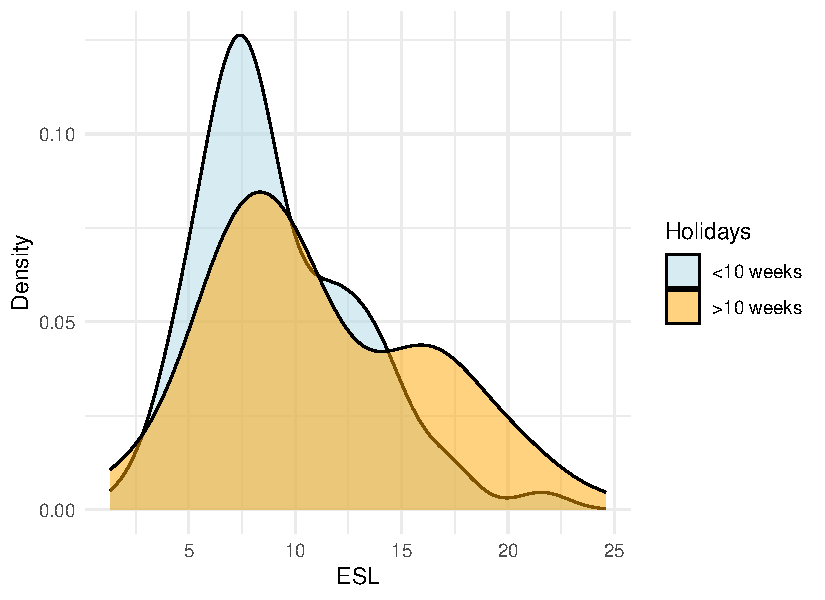
\includegraphics[width=1\textwidth,height=\textheight]{report_files/figure-pdf/graph_holydays_gr_10w-1.pdf}

}

\caption{Kernel Histogram Comparing ESL of Regions with more or less
than 10 Weeks of Holidays from School}

\end{figure}%

\subsubsection{Southern Europe}\label{southern-europe}

The other dummy variable used in the model is the region's membership in
the Southern European area. To examine potential differences in the
relationship between the rate of early school leavers and European
regions, a Chow test was conducted. The Chow test is utilized to
investigate whether there exists a significant structural break between
the regression model of Southern Europe region and a model with the rest
of the regions. This is because historically this region has profoundly
different characteristics than other European regions. We used to
identify them the division made by the
United\_Nations\_Statistics\_Division (n.d.).

\begin{figure}[H]

{\centering 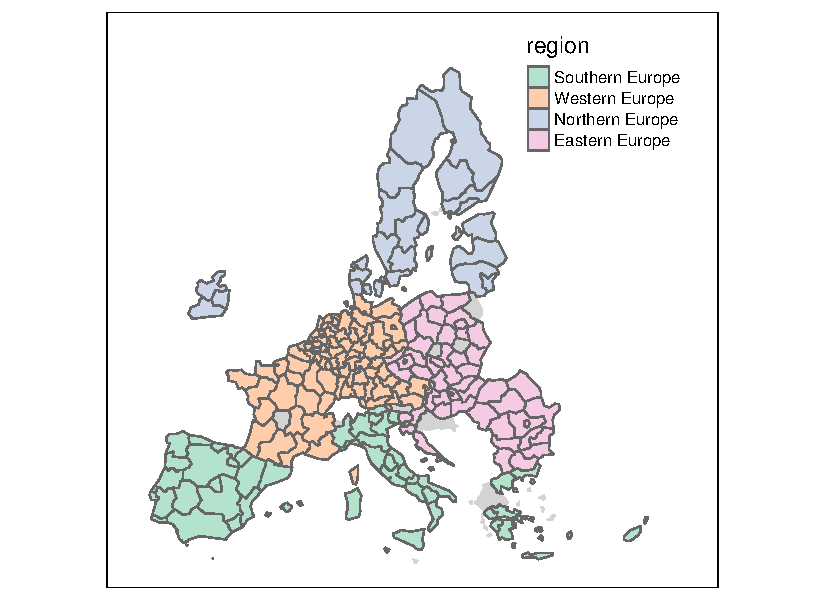
\includegraphics[width=1\textwidth,height=\textheight]{report_files/figure-pdf/mappa region-1.pdf}

}

\caption{European Regions}

\end{figure}%

\begin{longtable}[]{@{}rrrr@{}}
\caption{Summary of Chow Test}\tabularnewline
\toprule\noalign{}
F value & d.f.1 & d.f.2 & P value \\
\midrule\noalign{}
\endfirsthead
\toprule\noalign{}
F value & d.f.1 & d.f.2 & P value \\
\midrule\noalign{}
\endhead
\bottomrule\noalign{}
\endlastfoot
11.926 & 7 & 208 & 0 \\
\end{longtable}

The p-value of Chow's test was found to be highly significant, which is
why it was decided to adopt Southern Europe as a dummy variable.

\newpage{}

\begin{longtable}[]{@{}
  >{\raggedright\arraybackslash}p{(\columnwidth - 12\tabcolsep) * \real{0.1130}}
  >{\raggedright\arraybackslash}p{(\columnwidth - 12\tabcolsep) * \real{0.1478}}
  >{\raggedright\arraybackslash}p{(\columnwidth - 12\tabcolsep) * \real{0.1478}}
  >{\raggedright\arraybackslash}p{(\columnwidth - 12\tabcolsep) * \real{0.1478}}
  >{\raggedright\arraybackslash}p{(\columnwidth - 12\tabcolsep) * \real{0.1478}}
  >{\raggedright\arraybackslash}p{(\columnwidth - 12\tabcolsep) * \real{0.1478}}
  >{\raggedright\arraybackslash}p{(\columnwidth - 12\tabcolsep) * \real{0.1478}}@{}}
\caption{Summary of the Quantitative Predictors}\tabularnewline
\toprule\noalign{}
\endfirsthead
\endhead
\bottomrule\noalign{}
\endlastfoot
esl & Min. : 1.300 & 1st Qu.: 6.900 & Median : 8.700 & Mean : 9.922 &
3rd Qu.:12.575 & Max. :24.600 \\
disp\_inc & Min. : 8.164 & 1st Qu.:14.590 & Median :17.921 & Mean
:17.651 & 3rd Qu.:20.825 & Max. :28.289 \\
density & Min. : 0.0350 & 1st Qu.: 0.7248 & Median : 1.2350 & Mean :
3.6344 & 3rd Qu.: 2.6850 & Max. :76.6000 \\
unemployment & Min. : 1.700 & 1st Qu.: 3.200 & Median : 5.100 & Mean :
6.093 & 3rd Qu.: 7.475 & Max. :30.000 \\
HRST & Min. :21.60 & 1st Qu.:39.15 & Median :47.20 & Mean :46.40 & 3rd
Qu.:52.58 & Max. :72.90 \\
amLSE & Min. : 1.80 & 1st Qu.:11.93 & Median :17.55 & Mean :19.60 & 3rd
Qu.:24.85 & Max. :58.80 \\
tourism & Min. : 0.6838 & 1st Qu.: 2.7955 & Median : 4.3757 & Mean :
7.6196 & 3rd Qu.: 7.6543 & Max. :110.4065 \\
\end{longtable}

\begin{figure}[H]

{\centering 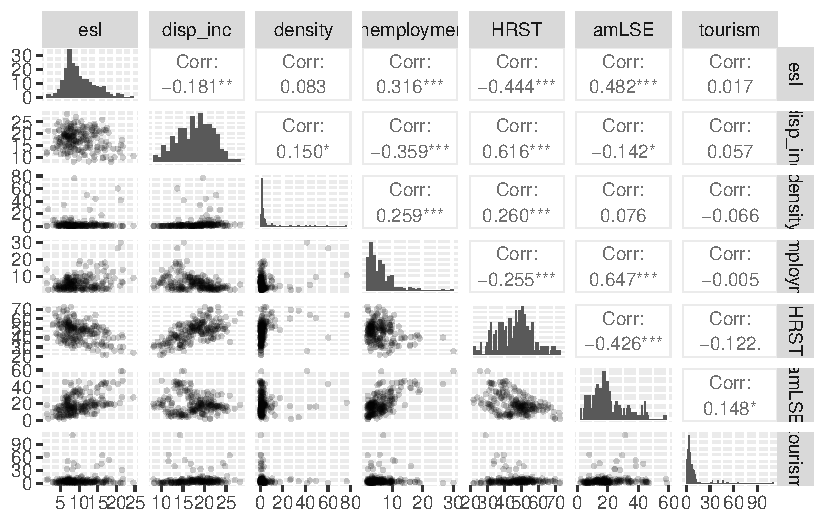
\includegraphics[width=1\textwidth,height=\textheight]{report_files/figure-pdf/correlation matrix-1.pdf}

}

\caption{Correlation Plot of Quantitative Predictors}

\end{figure}%

\section{Results}\label{results}

\subsection{Multiple Regression Model}\label{multiple-regression-model}

The primary objective was to analyze and predict the percentage of early
school leavers across various EU regions. To achieve this, a multiple
regression model was employed, with the response variable being the
percentage of early school leavers. The explanatory variables were
selected based on theoretical foundations and prior research indicating
their potential impact on early school leaving rates.

First of all, the model parameters were estimated using Ordinary Least
Squares (OLS) method and the overall model fit was evaluated using
R-squared and adjusted R-squared values.

Moreover, Variance Inflation Factors (VIFs) were calculated to check for
multicollinearity among the explanatory variables. Variables with high
VIFs were later removed to reduce multicollinearity. Various models were
compared using Adjusted RSquared criteria to select the most
parsimonious model that provided the best fit to the data. The model
coefficients were interpreted to understand the direction and magnitude
of the relationships

Finally, residual plots, normality tests and homoschedasticity test were
examined to ensure that the residuals were randomly distributed and did
not exhibit any patterns.

\subsubsection{Complete Regression}\label{complete-regression}

Initially, Early School Leaving was analyzed in relation to all
available explanatory variables. It was first decided to center the
quantitative explanatory variables (not the dummies, of course) such
that they all had for mean 0, to ensure greater interpretability in the
results. The multiple regression model was specified as: \[
\text{Early School Leavers} = \beta_0 + \beta_1 \text{Mean Disposable Income} + \beta_2 \text{Population Density} + \]
\[
+ \beta_3 \text{Unemployment Rate} + \beta_4 \text{Human Resources in Science and Technology} + \]
\[
+ \beta_5 \text{Over 25 with at most Lower Secondary Education}+ \beta_6 \text {Tourism} + \]
\[
+ \beta_7 \text {More than 10 weeks of Holyday from School} + \beta_8 \text {Southern Europe} + \epsilon{_i} \]

\newpage{}

We see that the significant covariates at the one-per-thousand level are
the percentage of workers working in science and technology, which have
a negative effect on school dropout, and the percentage of adults with
at most lower secondary education, which has a positive effect instead.

\global\setlength{\Oldarrayrulewidth}{\arrayrulewidth}

\global\setlength{\Oldtabcolsep}{\tabcolsep}

\setlength{\tabcolsep}{2pt}

\renewcommand*{\arraystretch}{1.5}



\providecommand{\ascline}[3]{\noalign{\global\arrayrulewidth #1}\arrayrulecolor[HTML]{#2}\cline{#3}}

\begin{longtable*}[c]{|p{1.56in}|p{0.88in}|p{1.29in}|p{0.75in}|p{0.75in}|p{0.40in}}



\ascline{1.5pt}{666666}{1-6}

\multicolumn{1}{>{\raggedright}m{\dimexpr 1.56in+0\tabcolsep}}{\textcolor[HTML]{000000}{\fontsize{11}{11}\selectfont{\global\setmainfont{Arial}{}}}} & \multicolumn{1}{>{\raggedleft}m{\dimexpr 0.88in+0\tabcolsep}}{\textcolor[HTML]{000000}{\fontsize{11}{11}\selectfont{\global\setmainfont{Arial}{Estimate}}}} & \multicolumn{1}{>{\raggedleft}m{\dimexpr 1.29in+0\tabcolsep}}{\textcolor[HTML]{000000}{\fontsize{11}{11}\selectfont{\global\setmainfont{Arial}{Standard\ Error}}}} & \multicolumn{1}{>{\raggedleft}m{\dimexpr 0.75in+0\tabcolsep}}{\textcolor[HTML]{000000}{\fontsize{11}{11}\selectfont{\global\setmainfont{Arial}{t\ value}}}} & \multicolumn{1}{>{\raggedleft}m{\dimexpr 0.75in+0\tabcolsep}}{\textcolor[HTML]{000000}{\fontsize{11}{11}\selectfont{\global\setmainfont{Arial}{Pr(>|t|)}}}} & \multicolumn{1}{>{\raggedright}m{\dimexpr 0.4in+0\tabcolsep}}{\textcolor[HTML]{000000}{\fontsize{11}{11}\selectfont{\global\setmainfont{Arial}{}}}} \\

\ascline{1.5pt}{666666}{1-6}\endfirsthead 

\ascline{1.5pt}{666666}{1-6}

\multicolumn{1}{>{\raggedright}m{\dimexpr 1.56in+0\tabcolsep}}{\textcolor[HTML]{000000}{\fontsize{11}{11}\selectfont{\global\setmainfont{Arial}{}}}} & \multicolumn{1}{>{\raggedleft}m{\dimexpr 0.88in+0\tabcolsep}}{\textcolor[HTML]{000000}{\fontsize{11}{11}\selectfont{\global\setmainfont{Arial}{Estimate}}}} & \multicolumn{1}{>{\raggedleft}m{\dimexpr 1.29in+0\tabcolsep}}{\textcolor[HTML]{000000}{\fontsize{11}{11}\selectfont{\global\setmainfont{Arial}{Standard\ Error}}}} & \multicolumn{1}{>{\raggedleft}m{\dimexpr 0.75in+0\tabcolsep}}{\textcolor[HTML]{000000}{\fontsize{11}{11}\selectfont{\global\setmainfont{Arial}{t\ value}}}} & \multicolumn{1}{>{\raggedleft}m{\dimexpr 0.75in+0\tabcolsep}}{\textcolor[HTML]{000000}{\fontsize{11}{11}\selectfont{\global\setmainfont{Arial}{Pr(>|t|)}}}} & \multicolumn{1}{>{\raggedright}m{\dimexpr 0.4in+0\tabcolsep}}{\textcolor[HTML]{000000}{\fontsize{11}{11}\selectfont{\global\setmainfont{Arial}{}}}} \\

\ascline{1.5pt}{666666}{1-6}\endhead



\multicolumn{1}{>{\raggedright}m{\dimexpr 1.56in+0\tabcolsep}}{\textcolor[HTML]{000000}{\fontsize{11}{11}\selectfont{\global\setmainfont{Arial}{(Intercept)}}}} & \multicolumn{1}{>{\raggedleft}m{\dimexpr 0.88in+0\tabcolsep}}{\textcolor[HTML]{000000}{\fontsize{11}{11}\selectfont{\global\setmainfont{Arial}{11.035}}}} & \multicolumn{1}{>{\raggedleft}m{\dimexpr 1.29in+0\tabcolsep}}{\textcolor[HTML]{000000}{\fontsize{11}{11}\selectfont{\global\setmainfont{Arial}{0.325}}}} & \multicolumn{1}{>{\raggedleft}m{\dimexpr 0.75in+0\tabcolsep}}{\textcolor[HTML]{000000}{\fontsize{11}{11}\selectfont{\global\setmainfont{Arial}{33.946}}}} & \multicolumn{1}{>{\raggedleft}m{\dimexpr 0.75in+0\tabcolsep}}{\textcolor[HTML]{000000}{\fontsize{11}{11}\selectfont{\global\setmainfont{Arial}{0.0000}}}} & \multicolumn{1}{>{\raggedright}m{\dimexpr 0.4in+0\tabcolsep}}{\textcolor[HTML]{000000}{\fontsize{11}{11}\selectfont{\global\setmainfont{Arial}{***}}}} \\





\multicolumn{1}{>{\raggedright}m{\dimexpr 1.56in+0\tabcolsep}}{\textcolor[HTML]{000000}{\fontsize{11}{11}\selectfont{\global\setmainfont{Arial}{disp\_inc}}}} & \multicolumn{1}{>{\raggedleft}m{\dimexpr 0.88in+0\tabcolsep}}{\textcolor[HTML]{000000}{\fontsize{11}{11}\selectfont{\global\setmainfont{Arial}{0.180}}}} & \multicolumn{1}{>{\raggedleft}m{\dimexpr 1.29in+0\tabcolsep}}{\textcolor[HTML]{000000}{\fontsize{11}{11}\selectfont{\global\setmainfont{Arial}{0.087}}}} & \multicolumn{1}{>{\raggedleft}m{\dimexpr 0.75in+0\tabcolsep}}{\textcolor[HTML]{000000}{\fontsize{11}{11}\selectfont{\global\setmainfont{Arial}{2.063}}}} & \multicolumn{1}{>{\raggedleft}m{\dimexpr 0.75in+0\tabcolsep}}{\textcolor[HTML]{000000}{\fontsize{11}{11}\selectfont{\global\setmainfont{Arial}{0.0403}}}} & \multicolumn{1}{>{\raggedright}m{\dimexpr 0.4in+0\tabcolsep}}{\textcolor[HTML]{000000}{\fontsize{11}{11}\selectfont{\global\setmainfont{Arial}{\ \ *}}}} \\





\multicolumn{1}{>{\raggedright}m{\dimexpr 1.56in+0\tabcolsep}}{\textcolor[HTML]{000000}{\fontsize{11}{11}\selectfont{\global\setmainfont{Arial}{density}}}} & \multicolumn{1}{>{\raggedleft}m{\dimexpr 0.88in+0\tabcolsep}}{\textcolor[HTML]{000000}{\fontsize{11}{11}\selectfont{\global\setmainfont{Arial}{0.047}}}} & \multicolumn{1}{>{\raggedleft}m{\dimexpr 1.29in+0\tabcolsep}}{\textcolor[HTML]{000000}{\fontsize{11}{11}\selectfont{\global\setmainfont{Arial}{0.028}}}} & \multicolumn{1}{>{\raggedleft}m{\dimexpr 0.75in+0\tabcolsep}}{\textcolor[HTML]{000000}{\fontsize{11}{11}\selectfont{\global\setmainfont{Arial}{1.701}}}} & \multicolumn{1}{>{\raggedleft}m{\dimexpr 0.75in+0\tabcolsep}}{\textcolor[HTML]{000000}{\fontsize{11}{11}\selectfont{\global\setmainfont{Arial}{0.0903}}}} & \multicolumn{1}{>{\raggedright}m{\dimexpr 0.4in+0\tabcolsep}}{\textcolor[HTML]{000000}{\fontsize{11}{11}\selectfont{\global\setmainfont{Arial}{\ \ .}}}} \\





\multicolumn{1}{>{\raggedright}m{\dimexpr 1.56in+0\tabcolsep}}{\textcolor[HTML]{000000}{\fontsize{11}{11}\selectfont{\global\setmainfont{Arial}{unemployment}}}} & \multicolumn{1}{>{\raggedleft}m{\dimexpr 0.88in+0\tabcolsep}}{\textcolor[HTML]{000000}{\fontsize{11}{11}\selectfont{\global\setmainfont{Arial}{0.105}}}} & \multicolumn{1}{>{\raggedleft}m{\dimexpr 1.29in+0\tabcolsep}}{\textcolor[HTML]{000000}{\fontsize{11}{11}\selectfont{\global\setmainfont{Arial}{0.086}}}} & \multicolumn{1}{>{\raggedleft}m{\dimexpr 0.75in+0\tabcolsep}}{\textcolor[HTML]{000000}{\fontsize{11}{11}\selectfont{\global\setmainfont{Arial}{1.230}}}} & \multicolumn{1}{>{\raggedleft}m{\dimexpr 0.75in+0\tabcolsep}}{\textcolor[HTML]{000000}{\fontsize{11}{11}\selectfont{\global\setmainfont{Arial}{0.2201}}}} & \multicolumn{1}{>{\raggedright}m{\dimexpr 0.4in+0\tabcolsep}}{\textcolor[HTML]{000000}{\fontsize{11}{11}\selectfont{\global\setmainfont{Arial}{\ \ \ }}}} \\





\multicolumn{1}{>{\raggedright}m{\dimexpr 1.56in+0\tabcolsep}}{\textcolor[HTML]{000000}{\fontsize{11}{11}\selectfont{\global\setmainfont{Arial}{HRST}}}} & \multicolumn{1}{>{\raggedleft}m{\dimexpr 0.88in+0\tabcolsep}}{\textcolor[HTML]{000000}{\fontsize{11}{11}\selectfont{\global\setmainfont{Arial}{-0.178}}}} & \multicolumn{1}{>{\raggedleft}m{\dimexpr 1.29in+0\tabcolsep}}{\textcolor[HTML]{000000}{\fontsize{11}{11}\selectfont{\global\setmainfont{Arial}{0.033}}}} & \multicolumn{1}{>{\raggedleft}m{\dimexpr 0.75in+0\tabcolsep}}{\textcolor[HTML]{000000}{\fontsize{11}{11}\selectfont{\global\setmainfont{Arial}{-5.364}}}} & \multicolumn{1}{>{\raggedleft}m{\dimexpr 0.75in+0\tabcolsep}}{\textcolor[HTML]{000000}{\fontsize{11}{11}\selectfont{\global\setmainfont{Arial}{0.0000}}}} & \multicolumn{1}{>{\raggedright}m{\dimexpr 0.4in+0\tabcolsep}}{\textcolor[HTML]{000000}{\fontsize{11}{11}\selectfont{\global\setmainfont{Arial}{***}}}} \\





\multicolumn{1}{>{\raggedright}m{\dimexpr 1.56in+0\tabcolsep}}{\textcolor[HTML]{000000}{\fontsize{11}{11}\selectfont{\global\setmainfont{Arial}{amLSE}}}} & \multicolumn{1}{>{\raggedleft}m{\dimexpr 0.88in+0\tabcolsep}}{\textcolor[HTML]{000000}{\fontsize{11}{11}\selectfont{\global\setmainfont{Arial}{0.261}}}} & \multicolumn{1}{>{\raggedleft}m{\dimexpr 1.29in+0\tabcolsep}}{\textcolor[HTML]{000000}{\fontsize{11}{11}\selectfont{\global\setmainfont{Arial}{0.037}}}} & \multicolumn{1}{>{\raggedleft}m{\dimexpr 0.75in+0\tabcolsep}}{\textcolor[HTML]{000000}{\fontsize{11}{11}\selectfont{\global\setmainfont{Arial}{7.151}}}} & \multicolumn{1}{>{\raggedleft}m{\dimexpr 0.75in+0\tabcolsep}}{\textcolor[HTML]{000000}{\fontsize{11}{11}\selectfont{\global\setmainfont{Arial}{0.0000}}}} & \multicolumn{1}{>{\raggedright}m{\dimexpr 0.4in+0\tabcolsep}}{\textcolor[HTML]{000000}{\fontsize{11}{11}\selectfont{\global\setmainfont{Arial}{***}}}} \\





\multicolumn{1}{>{\raggedright}m{\dimexpr 1.56in+0\tabcolsep}}{\textcolor[HTML]{000000}{\fontsize{11}{11}\selectfont{\global\setmainfont{Arial}{tourism}}}} & \multicolumn{1}{>{\raggedleft}m{\dimexpr 0.88in+0\tabcolsep}}{\textcolor[HTML]{000000}{\fontsize{11}{11}\selectfont{\global\setmainfont{Arial}{-0.001}}}} & \multicolumn{1}{>{\raggedleft}m{\dimexpr 1.29in+0\tabcolsep}}{\textcolor[HTML]{000000}{\fontsize{11}{11}\selectfont{\global\setmainfont{Arial}{0.019}}}} & \multicolumn{1}{>{\raggedleft}m{\dimexpr 0.75in+0\tabcolsep}}{\textcolor[HTML]{000000}{\fontsize{11}{11}\selectfont{\global\setmainfont{Arial}{-0.054}}}} & \multicolumn{1}{>{\raggedleft}m{\dimexpr 0.75in+0\tabcolsep}}{\textcolor[HTML]{000000}{\fontsize{11}{11}\selectfont{\global\setmainfont{Arial}{0.9571}}}} & \multicolumn{1}{>{\raggedright}m{\dimexpr 0.4in+0\tabcolsep}}{\textcolor[HTML]{000000}{\fontsize{11}{11}\selectfont{\global\setmainfont{Arial}{\ \ \ }}}} \\





\multicolumn{1}{>{\raggedright}m{\dimexpr 1.56in+0\tabcolsep}}{\textcolor[HTML]{000000}{\fontsize{11}{11}\selectfont{\global\setmainfont{Arial}{holydays\_gr\_10w1}}}} & \multicolumn{1}{>{\raggedleft}m{\dimexpr 0.88in+0\tabcolsep}}{\textcolor[HTML]{000000}{\fontsize{11}{11}\selectfont{\global\setmainfont{Arial}{1.514}}}} & \multicolumn{1}{>{\raggedleft}m{\dimexpr 1.29in+0\tabcolsep}}{\textcolor[HTML]{000000}{\fontsize{11}{11}\selectfont{\global\setmainfont{Arial}{0.841}}}} & \multicolumn{1}{>{\raggedleft}m{\dimexpr 0.75in+0\tabcolsep}}{\textcolor[HTML]{000000}{\fontsize{11}{11}\selectfont{\global\setmainfont{Arial}{1.799}}}} & \multicolumn{1}{>{\raggedleft}m{\dimexpr 0.75in+0\tabcolsep}}{\textcolor[HTML]{000000}{\fontsize{11}{11}\selectfont{\global\setmainfont{Arial}{0.0734}}}} & \multicolumn{1}{>{\raggedright}m{\dimexpr 0.4in+0\tabcolsep}}{\textcolor[HTML]{000000}{\fontsize{11}{11}\selectfont{\global\setmainfont{Arial}{\ \ .}}}} \\





\multicolumn{1}{>{\raggedright}m{\dimexpr 1.56in+0\tabcolsep}}{\textcolor[HTML]{000000}{\fontsize{11}{11}\selectfont{\global\setmainfont{Arial}{region1}}}} & \multicolumn{1}{>{\raggedleft}m{\dimexpr 0.88in+0\tabcolsep}}{\textcolor[HTML]{000000}{\fontsize{11}{11}\selectfont{\global\setmainfont{Arial}{-6.876}}}} & \multicolumn{1}{>{\raggedleft}m{\dimexpr 1.29in+0\tabcolsep}}{\textcolor[HTML]{000000}{\fontsize{11}{11}\selectfont{\global\setmainfont{Arial}{1.039}}}} & \multicolumn{1}{>{\raggedleft}m{\dimexpr 0.75in+0\tabcolsep}}{\textcolor[HTML]{000000}{\fontsize{11}{11}\selectfont{\global\setmainfont{Arial}{-6.620}}}} & \multicolumn{1}{>{\raggedleft}m{\dimexpr 0.75in+0\tabcolsep}}{\textcolor[HTML]{000000}{\fontsize{11}{11}\selectfont{\global\setmainfont{Arial}{0.0000}}}} & \multicolumn{1}{>{\raggedright}m{\dimexpr 0.4in+0\tabcolsep}}{\textcolor[HTML]{000000}{\fontsize{11}{11}\selectfont{\global\setmainfont{Arial}{***}}}} \\

\ascline{1.5pt}{666666}{1-6}



\multicolumn{6}{>{\raggedleft}m{\dimexpr 5.63in+10\tabcolsep}}{\textcolor[HTML]{000000}{\fontsize{11}{11}\selectfont{\global\setmainfont{Arial}{\textit{Signif.\ codes:\ 0\ <=\ '***'\ <\ 0.001\ <\ '**'\ <\ 0.01\ <\ '*'\ <\ 0.05}}}}} \\





\multicolumn{6}{>{\raggedright}m{\dimexpr 5.63in+10\tabcolsep}}{\textcolor[HTML]{000000}{\fontsize{11}{11}\selectfont{\global\setmainfont{Arial}{}}}} \\





\multicolumn{6}{>{\raggedright}m{\dimexpr 5.63in+10\tabcolsep}}{\textcolor[HTML]{000000}{\fontsize{11}{11}\selectfont{\global\setmainfont{Arial}{Residual\ standard\ error:\ 3.262\ on\ 213\ degrees\ of\ freedom}}}} \\





\multicolumn{6}{>{\raggedright}m{\dimexpr 5.63in+10\tabcolsep}}{\textcolor[HTML]{000000}{\fontsize{11}{11}\selectfont{\global\setmainfont{Arial}{Multiple\ R-squared:\ 0.4695,\ Adjusted\ R-squared:\ 0.4496}}}} \\





\multicolumn{6}{>{\raggedright}m{\dimexpr 5.63in+10\tabcolsep}}{\textcolor[HTML]{000000}{\fontsize{11}{11}\selectfont{\global\setmainfont{Arial}{F-statistic:\ 23.56\ on\ 213\ and\ 8\ DF,\ p-value:\ 0.0000}}}} \\





\end{longtable*}



\arrayrulecolor[HTML]{000000}

\global\setlength{\arrayrulewidth}{\Oldarrayrulewidth}

\global\setlength{\tabcolsep}{\Oldtabcolsep}

\renewcommand*{\arraystretch}{1}

In this model, the residuals are symmetrically distributed around zero,
with no extreme values suggesting outliers. Furthermore, the leverage
statistics, which measure the influence of individual data points on the
regression coefficients, do not show any observations with
disproportionately high leverage

\begin{figure}[H]

{\centering 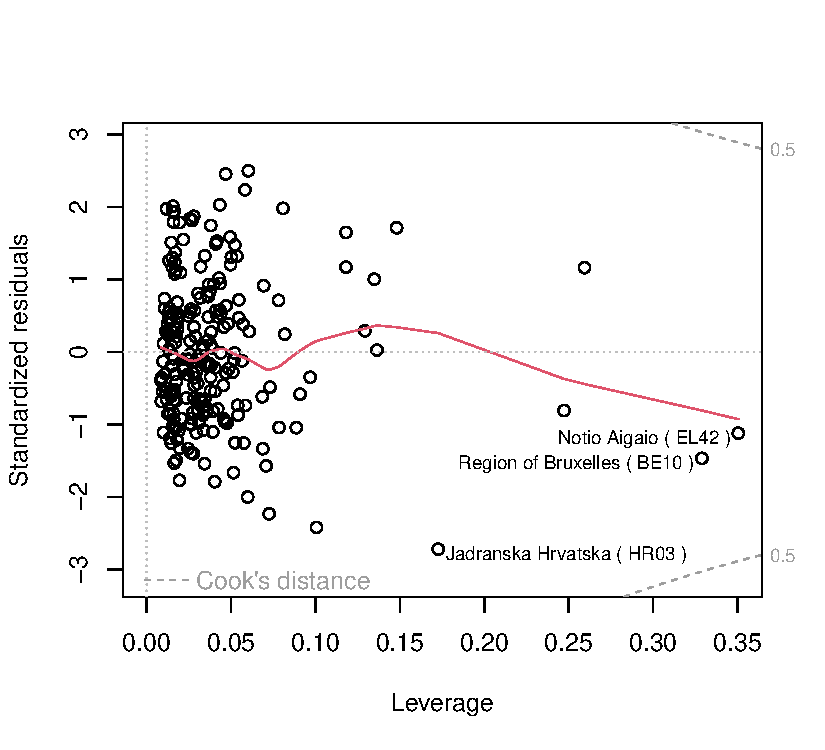
\includegraphics[width=1\textwidth,height=\textheight]{report_files/figure-pdf/residualsvsleverage-1.pdf}

}

\caption{Residuals vs Leverage}

\end{figure}%

The residual diagnostics indicated that the residuals follow a normal
distribution, as confirmed by the Normality Tests.

\begin{figure}[H]

{\centering 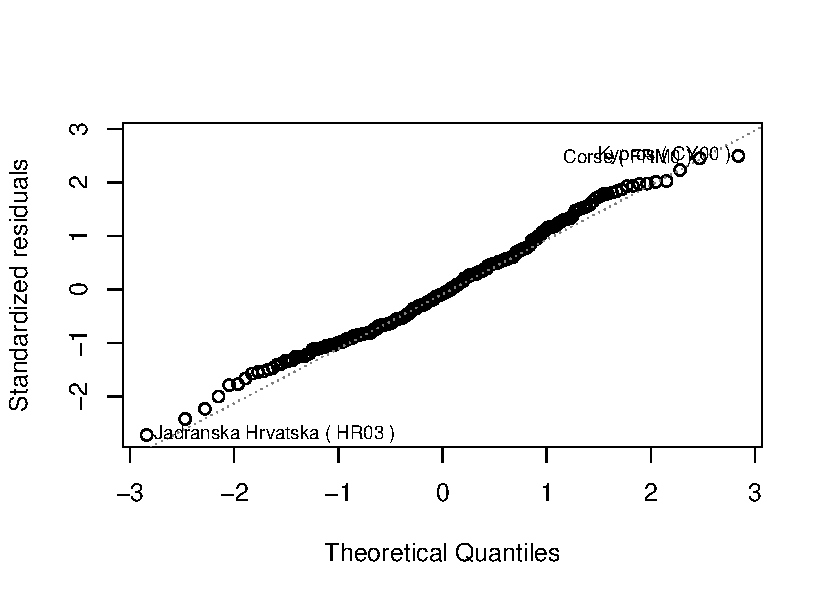
\includegraphics[width=1\textwidth,height=\textheight]{report_files/figure-pdf/qqplot-1.pdf}

}

\caption{QQ-Plot}

\end{figure}%

\begin{figure}[H]

{\centering 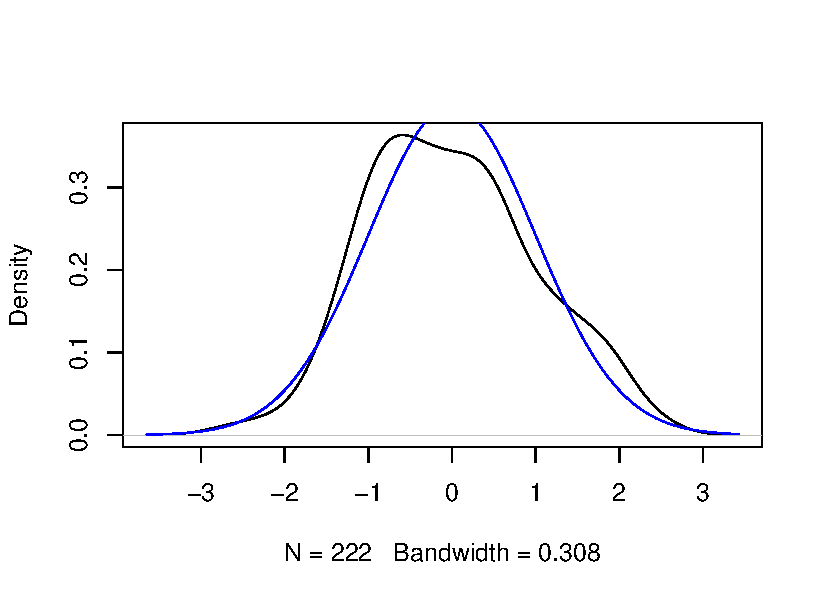
\includegraphics[width=1\textwidth,height=\textheight]{report_files/figure-pdf/normale-1.pdf}

}

\caption{Kernel Hitogram of Residuals}

\end{figure}%

\begin{longtable}[]{@{}rrr@{}}
\caption{Normality Tests of Residuals}\tabularnewline
\toprule\noalign{}
Shapiro-Wilk & Jarque Bera & Kolmogorov-Smirnov \\
\midrule\noalign{}
\endfirsthead
\toprule\noalign{}
Shapiro-Wilk & Jarque Bera & Kolmogorov-Smirnov \\
\midrule\noalign{}
\endhead
\bottomrule\noalign{}
\endlastfoot
0.069 & 0.23 & 0.488 \\
\end{longtable}

To investigate the presence of heteroscedasticity in our regression
model, we applied the Breusch-Pagan test to evaluate whether the
variance of the residuals from a regression model depends on the values
of the dependent variable.

\begin{figure}[H]

{\centering 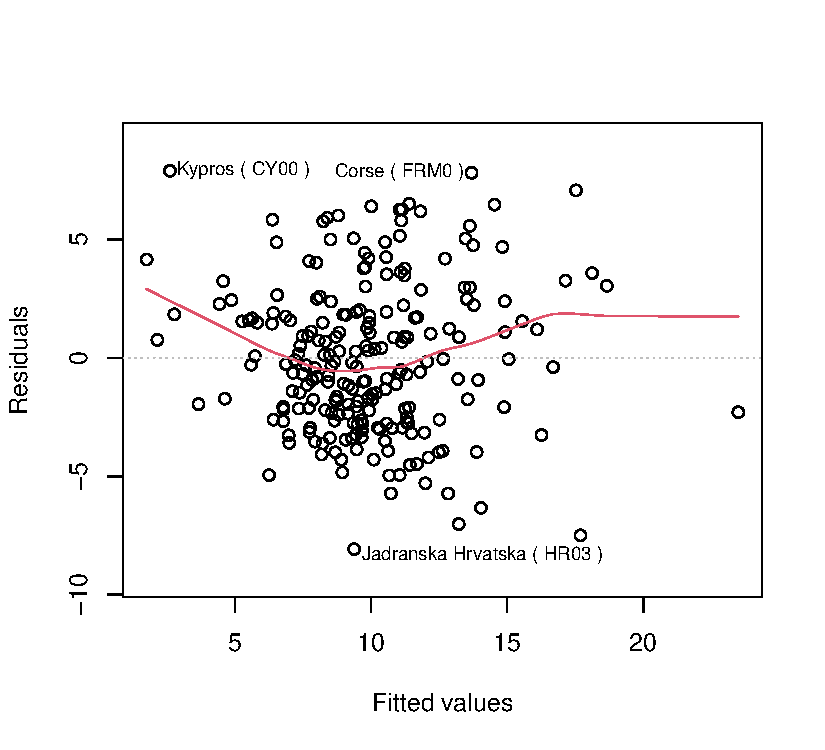
\includegraphics[width=1\textwidth,height=\textheight]{report_files/figure-pdf/residualsvsfitted-1.pdf}

}

\caption{Residuals vs Fitted Values}

\end{figure}%

The Breusch-Pagan test yielded a test statistic of 20.36 with a
corresponding p-value of 0.009, indicating significant evidence of
heteroscedasticity at the conventional significance level of 0.05. Since
heteroscedasticity is present, it could have lead to inefficient
estimates and biased standard errors. Consequently, the assumption of
homoscedasticity is violated, and remedial measures are necessary.

\begin{longtable}[]{@{}rrr@{}}
\caption{Homoschedasticity Tests of Residuals}\tabularnewline
\toprule\noalign{}
BP.BP & df.df & p-value.BP \\
\midrule\noalign{}
\endfirsthead
\toprule\noalign{}
BP.BP & df.df & p-value.BP \\
\midrule\noalign{}
\endhead
\bottomrule\noalign{}
\endlastfoot
20.363 & 8 & 0.009 \\
\end{longtable}

To address the issue, we employed Feasible Generalized Least Squares
(FGLS). First, we estimated the variance of the error terms by
regressing the squared residuals from the initial model on the set of
independent variables. This step provides an estimate of the predicted
variance of the residuals, which we then used to calculate weights for
the FGLS model. The weights were computed as the inverse of the
predicted variance, allowing us to apply the appropriate transformation
to achieve homoscedasticity.

We then refitted the model using these weights to obtain the FGLS
estimates. This transformation effectively stabilizes the variance of
the error terms, correcting for heteroscedasticity and enhancing the
efficiency of the model estimates.

\global\setlength{\Oldarrayrulewidth}{\arrayrulewidth}

\global\setlength{\Oldtabcolsep}{\tabcolsep}

\setlength{\tabcolsep}{2pt}

\renewcommand*{\arraystretch}{1.5}



\providecommand{\ascline}[3]{\noalign{\global\arrayrulewidth #1}\arrayrulecolor[HTML]{#2}\cline{#3}}

\begin{longtable*}[c]{|p{1.56in}|p{0.88in}|p{1.29in}|p{0.75in}|p{0.75in}|p{0.40in}}



\ascline{1.5pt}{666666}{1-6}

\multicolumn{1}{>{\raggedright}m{\dimexpr 1.56in+0\tabcolsep}}{\textcolor[HTML]{000000}{\fontsize{11}{11}\selectfont{\global\setmainfont{Arial}{}}}} & \multicolumn{1}{>{\raggedleft}m{\dimexpr 0.88in+0\tabcolsep}}{\textcolor[HTML]{000000}{\fontsize{11}{11}\selectfont{\global\setmainfont{Arial}{Estimate}}}} & \multicolumn{1}{>{\raggedleft}m{\dimexpr 1.29in+0\tabcolsep}}{\textcolor[HTML]{000000}{\fontsize{11}{11}\selectfont{\global\setmainfont{Arial}{Standard\ Error}}}} & \multicolumn{1}{>{\raggedleft}m{\dimexpr 0.75in+0\tabcolsep}}{\textcolor[HTML]{000000}{\fontsize{11}{11}\selectfont{\global\setmainfont{Arial}{t\ value}}}} & \multicolumn{1}{>{\raggedleft}m{\dimexpr 0.75in+0\tabcolsep}}{\textcolor[HTML]{000000}{\fontsize{11}{11}\selectfont{\global\setmainfont{Arial}{Pr(>|t|)}}}} & \multicolumn{1}{>{\raggedright}m{\dimexpr 0.4in+0\tabcolsep}}{\textcolor[HTML]{000000}{\fontsize{11}{11}\selectfont{\global\setmainfont{Arial}{}}}} \\

\ascline{1.5pt}{666666}{1-6}\endfirsthead 

\ascline{1.5pt}{666666}{1-6}

\multicolumn{1}{>{\raggedright}m{\dimexpr 1.56in+0\tabcolsep}}{\textcolor[HTML]{000000}{\fontsize{11}{11}\selectfont{\global\setmainfont{Arial}{}}}} & \multicolumn{1}{>{\raggedleft}m{\dimexpr 0.88in+0\tabcolsep}}{\textcolor[HTML]{000000}{\fontsize{11}{11}\selectfont{\global\setmainfont{Arial}{Estimate}}}} & \multicolumn{1}{>{\raggedleft}m{\dimexpr 1.29in+0\tabcolsep}}{\textcolor[HTML]{000000}{\fontsize{11}{11}\selectfont{\global\setmainfont{Arial}{Standard\ Error}}}} & \multicolumn{1}{>{\raggedleft}m{\dimexpr 0.75in+0\tabcolsep}}{\textcolor[HTML]{000000}{\fontsize{11}{11}\selectfont{\global\setmainfont{Arial}{t\ value}}}} & \multicolumn{1}{>{\raggedleft}m{\dimexpr 0.75in+0\tabcolsep}}{\textcolor[HTML]{000000}{\fontsize{11}{11}\selectfont{\global\setmainfont{Arial}{Pr(>|t|)}}}} & \multicolumn{1}{>{\raggedright}m{\dimexpr 0.4in+0\tabcolsep}}{\textcolor[HTML]{000000}{\fontsize{11}{11}\selectfont{\global\setmainfont{Arial}{}}}} \\

\ascline{1.5pt}{666666}{1-6}\endhead



\multicolumn{1}{>{\raggedright}m{\dimexpr 1.56in+0\tabcolsep}}{\textcolor[HTML]{000000}{\fontsize{11}{11}\selectfont{\global\setmainfont{Arial}{(Intercept)}}}} & \multicolumn{1}{>{\raggedleft}m{\dimexpr 0.88in+0\tabcolsep}}{\textcolor[HTML]{000000}{\fontsize{11}{11}\selectfont{\global\setmainfont{Arial}{10.911}}}} & \multicolumn{1}{>{\raggedleft}m{\dimexpr 1.29in+0\tabcolsep}}{\textcolor[HTML]{000000}{\fontsize{11}{11}\selectfont{\global\setmainfont{Arial}{0.318}}}} & \multicolumn{1}{>{\raggedleft}m{\dimexpr 0.75in+0\tabcolsep}}{\textcolor[HTML]{000000}{\fontsize{11}{11}\selectfont{\global\setmainfont{Arial}{34.312}}}} & \multicolumn{1}{>{\raggedleft}m{\dimexpr 0.75in+0\tabcolsep}}{\textcolor[HTML]{000000}{\fontsize{11}{11}\selectfont{\global\setmainfont{Arial}{0.0000}}}} & \multicolumn{1}{>{\raggedright}m{\dimexpr 0.4in+0\tabcolsep}}{\textcolor[HTML]{000000}{\fontsize{11}{11}\selectfont{\global\setmainfont{Arial}{***}}}} \\





\multicolumn{1}{>{\raggedright}m{\dimexpr 1.56in+0\tabcolsep}}{\textcolor[HTML]{000000}{\fontsize{11}{11}\selectfont{\global\setmainfont{Arial}{disp\_inc}}}} & \multicolumn{1}{>{\raggedleft}m{\dimexpr 0.88in+0\tabcolsep}}{\textcolor[HTML]{000000}{\fontsize{11}{11}\selectfont{\global\setmainfont{Arial}{0.161}}}} & \multicolumn{1}{>{\raggedleft}m{\dimexpr 1.29in+0\tabcolsep}}{\textcolor[HTML]{000000}{\fontsize{11}{11}\selectfont{\global\setmainfont{Arial}{0.085}}}} & \multicolumn{1}{>{\raggedleft}m{\dimexpr 0.75in+0\tabcolsep}}{\textcolor[HTML]{000000}{\fontsize{11}{11}\selectfont{\global\setmainfont{Arial}{1.885}}}} & \multicolumn{1}{>{\raggedleft}m{\dimexpr 0.75in+0\tabcolsep}}{\textcolor[HTML]{000000}{\fontsize{11}{11}\selectfont{\global\setmainfont{Arial}{0.0609}}}} & \multicolumn{1}{>{\raggedright}m{\dimexpr 0.4in+0\tabcolsep}}{\textcolor[HTML]{000000}{\fontsize{11}{11}\selectfont{\global\setmainfont{Arial}{\ \ .}}}} \\





\multicolumn{1}{>{\raggedright}m{\dimexpr 1.56in+0\tabcolsep}}{\textcolor[HTML]{000000}{\fontsize{11}{11}\selectfont{\global\setmainfont{Arial}{density}}}} & \multicolumn{1}{>{\raggedleft}m{\dimexpr 0.88in+0\tabcolsep}}{\textcolor[HTML]{000000}{\fontsize{11}{11}\selectfont{\global\setmainfont{Arial}{0.045}}}} & \multicolumn{1}{>{\raggedleft}m{\dimexpr 1.29in+0\tabcolsep}}{\textcolor[HTML]{000000}{\fontsize{11}{11}\selectfont{\global\setmainfont{Arial}{0.026}}}} & \multicolumn{1}{>{\raggedleft}m{\dimexpr 0.75in+0\tabcolsep}}{\textcolor[HTML]{000000}{\fontsize{11}{11}\selectfont{\global\setmainfont{Arial}{1.722}}}} & \multicolumn{1}{>{\raggedleft}m{\dimexpr 0.75in+0\tabcolsep}}{\textcolor[HTML]{000000}{\fontsize{11}{11}\selectfont{\global\setmainfont{Arial}{0.0864}}}} & \multicolumn{1}{>{\raggedright}m{\dimexpr 0.4in+0\tabcolsep}}{\textcolor[HTML]{000000}{\fontsize{11}{11}\selectfont{\global\setmainfont{Arial}{\ \ .}}}} \\





\multicolumn{1}{>{\raggedright}m{\dimexpr 1.56in+0\tabcolsep}}{\textcolor[HTML]{000000}{\fontsize{11}{11}\selectfont{\global\setmainfont{Arial}{unemployment}}}} & \multicolumn{1}{>{\raggedleft}m{\dimexpr 0.88in+0\tabcolsep}}{\textcolor[HTML]{000000}{\fontsize{11}{11}\selectfont{\global\setmainfont{Arial}{0.102}}}} & \multicolumn{1}{>{\raggedleft}m{\dimexpr 1.29in+0\tabcolsep}}{\textcolor[HTML]{000000}{\fontsize{11}{11}\selectfont{\global\setmainfont{Arial}{0.086}}}} & \multicolumn{1}{>{\raggedleft}m{\dimexpr 0.75in+0\tabcolsep}}{\textcolor[HTML]{000000}{\fontsize{11}{11}\selectfont{\global\setmainfont{Arial}{1.194}}}} & \multicolumn{1}{>{\raggedleft}m{\dimexpr 0.75in+0\tabcolsep}}{\textcolor[HTML]{000000}{\fontsize{11}{11}\selectfont{\global\setmainfont{Arial}{0.2339}}}} & \multicolumn{1}{>{\raggedright}m{\dimexpr 0.4in+0\tabcolsep}}{\textcolor[HTML]{000000}{\fontsize{11}{11}\selectfont{\global\setmainfont{Arial}{\ \ \ }}}} \\





\multicolumn{1}{>{\raggedright}m{\dimexpr 1.56in+0\tabcolsep}}{\textcolor[HTML]{000000}{\fontsize{11}{11}\selectfont{\global\setmainfont{Arial}{HRST}}}} & \multicolumn{1}{>{\raggedleft}m{\dimexpr 0.88in+0\tabcolsep}}{\textcolor[HTML]{000000}{\fontsize{11}{11}\selectfont{\global\setmainfont{Arial}{-0.147}}}} & \multicolumn{1}{>{\raggedleft}m{\dimexpr 1.29in+0\tabcolsep}}{\textcolor[HTML]{000000}{\fontsize{11}{11}\selectfont{\global\setmainfont{Arial}{0.031}}}} & \multicolumn{1}{>{\raggedleft}m{\dimexpr 0.75in+0\tabcolsep}}{\textcolor[HTML]{000000}{\fontsize{11}{11}\selectfont{\global\setmainfont{Arial}{-4.787}}}} & \multicolumn{1}{>{\raggedleft}m{\dimexpr 0.75in+0\tabcolsep}}{\textcolor[HTML]{000000}{\fontsize{11}{11}\selectfont{\global\setmainfont{Arial}{0.0000}}}} & \multicolumn{1}{>{\raggedright}m{\dimexpr 0.4in+0\tabcolsep}}{\textcolor[HTML]{000000}{\fontsize{11}{11}\selectfont{\global\setmainfont{Arial}{***}}}} \\





\multicolumn{1}{>{\raggedright}m{\dimexpr 1.56in+0\tabcolsep}}{\textcolor[HTML]{000000}{\fontsize{11}{11}\selectfont{\global\setmainfont{Arial}{amLSE}}}} & \multicolumn{1}{>{\raggedleft}m{\dimexpr 0.88in+0\tabcolsep}}{\textcolor[HTML]{000000}{\fontsize{11}{11}\selectfont{\global\setmainfont{Arial}{0.247}}}} & \multicolumn{1}{>{\raggedleft}m{\dimexpr 1.29in+0\tabcolsep}}{\textcolor[HTML]{000000}{\fontsize{11}{11}\selectfont{\global\setmainfont{Arial}{0.034}}}} & \multicolumn{1}{>{\raggedleft}m{\dimexpr 0.75in+0\tabcolsep}}{\textcolor[HTML]{000000}{\fontsize{11}{11}\selectfont{\global\setmainfont{Arial}{7.311}}}} & \multicolumn{1}{>{\raggedleft}m{\dimexpr 0.75in+0\tabcolsep}}{\textcolor[HTML]{000000}{\fontsize{11}{11}\selectfont{\global\setmainfont{Arial}{0.0000}}}} & \multicolumn{1}{>{\raggedright}m{\dimexpr 0.4in+0\tabcolsep}}{\textcolor[HTML]{000000}{\fontsize{11}{11}\selectfont{\global\setmainfont{Arial}{***}}}} \\





\multicolumn{1}{>{\raggedright}m{\dimexpr 1.56in+0\tabcolsep}}{\textcolor[HTML]{000000}{\fontsize{11}{11}\selectfont{\global\setmainfont{Arial}{tourism}}}} & \multicolumn{1}{>{\raggedleft}m{\dimexpr 0.88in+0\tabcolsep}}{\textcolor[HTML]{000000}{\fontsize{11}{11}\selectfont{\global\setmainfont{Arial}{0.008}}}} & \multicolumn{1}{>{\raggedleft}m{\dimexpr 1.29in+0\tabcolsep}}{\textcolor[HTML]{000000}{\fontsize{11}{11}\selectfont{\global\setmainfont{Arial}{0.027}}}} & \multicolumn{1}{>{\raggedleft}m{\dimexpr 0.75in+0\tabcolsep}}{\textcolor[HTML]{000000}{\fontsize{11}{11}\selectfont{\global\setmainfont{Arial}{0.312}}}} & \multicolumn{1}{>{\raggedleft}m{\dimexpr 0.75in+0\tabcolsep}}{\textcolor[HTML]{000000}{\fontsize{11}{11}\selectfont{\global\setmainfont{Arial}{0.7555}}}} & \multicolumn{1}{>{\raggedright}m{\dimexpr 0.4in+0\tabcolsep}}{\textcolor[HTML]{000000}{\fontsize{11}{11}\selectfont{\global\setmainfont{Arial}{\ \ \ }}}} \\





\multicolumn{1}{>{\raggedright}m{\dimexpr 1.56in+0\tabcolsep}}{\textcolor[HTML]{000000}{\fontsize{11}{11}\selectfont{\global\setmainfont{Arial}{holydays\_gr\_10w1}}}} & \multicolumn{1}{>{\raggedleft}m{\dimexpr 0.88in+0\tabcolsep}}{\textcolor[HTML]{000000}{\fontsize{11}{11}\selectfont{\global\setmainfont{Arial}{1.599}}}} & \multicolumn{1}{>{\raggedleft}m{\dimexpr 1.29in+0\tabcolsep}}{\textcolor[HTML]{000000}{\fontsize{11}{11}\selectfont{\global\setmainfont{Arial}{0.820}}}} & \multicolumn{1}{>{\raggedleft}m{\dimexpr 0.75in+0\tabcolsep}}{\textcolor[HTML]{000000}{\fontsize{11}{11}\selectfont{\global\setmainfont{Arial}{1.949}}}} & \multicolumn{1}{>{\raggedleft}m{\dimexpr 0.75in+0\tabcolsep}}{\textcolor[HTML]{000000}{\fontsize{11}{11}\selectfont{\global\setmainfont{Arial}{0.0526}}}} & \multicolumn{1}{>{\raggedright}m{\dimexpr 0.4in+0\tabcolsep}}{\textcolor[HTML]{000000}{\fontsize{11}{11}\selectfont{\global\setmainfont{Arial}{\ \ .}}}} \\





\multicolumn{1}{>{\raggedright}m{\dimexpr 1.56in+0\tabcolsep}}{\textcolor[HTML]{000000}{\fontsize{11}{11}\selectfont{\global\setmainfont{Arial}{region1}}}} & \multicolumn{1}{>{\raggedleft}m{\dimexpr 0.88in+0\tabcolsep}}{\textcolor[HTML]{000000}{\fontsize{11}{11}\selectfont{\global\setmainfont{Arial}{-6.496}}}} & \multicolumn{1}{>{\raggedleft}m{\dimexpr 1.29in+0\tabcolsep}}{\textcolor[HTML]{000000}{\fontsize{11}{11}\selectfont{\global\setmainfont{Arial}{0.912}}}} & \multicolumn{1}{>{\raggedleft}m{\dimexpr 0.75in+0\tabcolsep}}{\textcolor[HTML]{000000}{\fontsize{11}{11}\selectfont{\global\setmainfont{Arial}{-7.123}}}} & \multicolumn{1}{>{\raggedleft}m{\dimexpr 0.75in+0\tabcolsep}}{\textcolor[HTML]{000000}{\fontsize{11}{11}\selectfont{\global\setmainfont{Arial}{0.0000}}}} & \multicolumn{1}{>{\raggedright}m{\dimexpr 0.4in+0\tabcolsep}}{\textcolor[HTML]{000000}{\fontsize{11}{11}\selectfont{\global\setmainfont{Arial}{***}}}} \\

\ascline{1.5pt}{666666}{1-6}



\multicolumn{6}{>{\raggedleft}m{\dimexpr 5.63in+10\tabcolsep}}{\textcolor[HTML]{000000}{\fontsize{11}{11}\selectfont{\global\setmainfont{Arial}{\textit{Signif.\ codes:\ 0\ <=\ '***'\ <\ 0.001\ <\ '**'\ <\ 0.01\ <\ '*'\ <\ 0.05}}}}} \\





\multicolumn{6}{>{\raggedright}m{\dimexpr 5.63in+10\tabcolsep}}{\textcolor[HTML]{000000}{\fontsize{11}{11}\selectfont{\global\setmainfont{Arial}{}}}} \\





\multicolumn{6}{>{\raggedright}m{\dimexpr 5.63in+10\tabcolsep}}{\textcolor[HTML]{000000}{\fontsize{11}{11}\selectfont{\global\setmainfont{Arial}{Residual\ standard\ error:\ 1.025\ on\ 213\ degrees\ of\ freedom}}}} \\





\multicolumn{6}{>{\raggedright}m{\dimexpr 5.63in+10\tabcolsep}}{\textcolor[HTML]{000000}{\fontsize{11}{11}\selectfont{\global\setmainfont{Arial}{Multiple\ R-squared:\ 0.5088,\ Adjusted\ R-squared:\ 0.4904}}}} \\





\multicolumn{6}{>{\raggedright}m{\dimexpr 5.63in+10\tabcolsep}}{\textcolor[HTML]{000000}{\fontsize{11}{11}\selectfont{\global\setmainfont{Arial}{F-statistic:\ 27.58\ on\ 213\ and\ 8\ DF,\ p-value:\ 0.0000}}}} \\





\end{longtable*}



\arrayrulecolor[HTML]{000000}

\global\setlength{\arrayrulewidth}{\Oldarrayrulewidth}

\global\setlength{\tabcolsep}{\Oldtabcolsep}

\renewcommand*{\arraystretch}{1}

FGLS were successfully corrected for heteroscedasticity as confirmed by
the Breusch-Pagan test showing a p-value of 0.486. However, now the
residuals deviate from a normal distribution. Additionally, we conducted
the Durbin-Watson test to check for autocorrelation in the residuals.
The results of this test were significant, suggesting that there is
evidence of autocorrelation in the residuals. This result suggests that
while FGLS addressed the heteroscedasticity issue, the normality
assumption and incorrelation of residuals still requires attention.

\begin{longtable}[]{@{}
  >{\raggedleft\arraybackslash}p{(\columnwidth - 4\tabcolsep) * \real{0.3333}}
  >{\raggedleft\arraybackslash}p{(\columnwidth - 4\tabcolsep) * \real{0.3846}}
  >{\raggedleft\arraybackslash}p{(\columnwidth - 4\tabcolsep) * \real{0.2821}}@{}}
\caption{Tests for FGLS}\tabularnewline
\toprule\noalign{}
\begin{minipage}[b]{\linewidth}\raggedleft
Shapiro-Wilk Test p-value
\end{minipage} & \begin{minipage}[b]{\linewidth}\raggedleft
Breusch-Pagan Test p-value.BP
\end{minipage} & \begin{minipage}[b]{\linewidth}\raggedleft
Durbin-Watson p-value
\end{minipage} \\
\midrule\noalign{}
\endfirsthead
\toprule\noalign{}
\begin{minipage}[b]{\linewidth}\raggedleft
Shapiro-Wilk Test p-value
\end{minipage} & \begin{minipage}[b]{\linewidth}\raggedleft
Breusch-Pagan Test p-value.BP
\end{minipage} & \begin{minipage}[b]{\linewidth}\raggedleft
Durbin-Watson p-value
\end{minipage} \\
\midrule\noalign{}
\endhead
\bottomrule\noalign{}
\endlastfoot
0.012 & 0.486 & 0 \\
\end{longtable}

The significant autocorrelation was attributed to the geographical
closeness of the regions in our dataset. This spatial autocorrelation
undermined the effectiveness of FGLS in correcting the issues at hand.

\begin{figure}[H]

{\centering 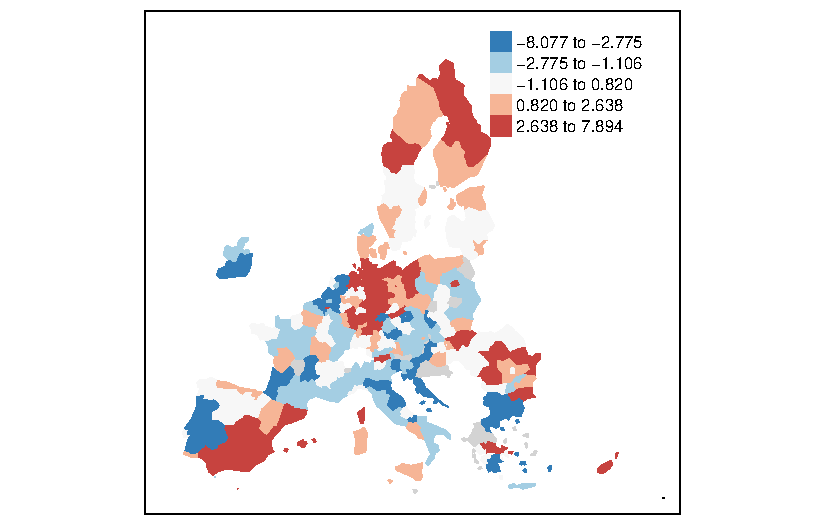
\includegraphics[width=1\textwidth,height=\textheight]{report_files/figure-pdf/redis_map-1.pdf}

}

\caption{Map of Model's Residuals}

\end{figure}%

To address both the autocorrelation and non-normality of residuals, we
opted to sample the dataset, abandoning the FGLS approach. The sampling
aimed to reduce the spatial proximity among observations, which
contributed to the observed autocorrelation. Specifically, we selected
100 random observations from the original dataset and fitted a new
linear model. The p-value of the Shapiro-Wilk Test was 0.0416,
indicating that the residuals still deviate from normality but to a
lesser extent than in the full dataset. However heteroscedasticity and
autocorrelation are not a significant issue in the model sampled
dataset.

\begin{longtable}[]{@{}rrr@{}}
\caption{Sample dataset model tests}\tabularnewline
\toprule\noalign{}
Shapiro-Wilk & Breusch-Pagan.BP & Durbin-Watson \\
\midrule\noalign{}
\endfirsthead
\toprule\noalign{}
Shapiro-Wilk & Breusch-Pagan.BP & Durbin-Watson \\
\midrule\noalign{}
\endhead
\bottomrule\noalign{}
\endlastfoot
0.042 & 0.48 & 0.076 \\
\end{longtable}

To summarize, in the OLS model applied to the entire dataset density has
a small but statistically significant positive effect on ESL, with a
coefficient of 0.047 significant at the 10\% level. While in the OLS
S.D. model applied to a randomly sampled subset of the dataset, the
coefficient for MDI increases to 0.357 and is significant at the 1\%
level. Unemployment also becomes significant in the sampled dataset
model, with a coefficient of 0.501 significant at the 1\% level.

\begin{verbatim}

==============================================
                      Dependent variable:     
                 -----------------------------
                              esl             
                 OLS S.E.    FGLS    OLS S.D. 
                    (1)       (2)       (3)   
----------------------------------------------
disp_inc          0.180**   0.161*   0.357*** 
                  (0.087)   (0.085)   (0.123) 
                                              
density           0.047*    0.045*    -0.015  
                  (0.028)   (0.026)   (0.049) 
                                              
unemployment       0.105     0.102   0.501*** 
                  (0.086)   (0.086)   (0.145) 
                                              
HRST             -0.178*** -0.147*** -0.189***
                  (0.033)   (0.031)   (0.043) 
                                              
amLSE            0.261***  0.247***  0.181*** 
                  (0.037)   (0.034)   (0.049) 
                                              
tourism           -0.001     0.008     0.016  
                  (0.019)   (0.027)   (0.023) 
                                              
holydays_gr_10w1  1.514*    1.599*   3.339*** 
                  (0.841)   (0.820)   (1.183) 
                                              
region1          -6.876*** -6.496*** -7.965***
                  (1.039)   (0.912)   (1.475) 
                                              
Constant         11.035*** 10.911*** 10.772***
                  (0.325)   (0.318)   (0.468) 
                                              
----------------------------------------------
Observations        222       222       100   
R2                 0.469     0.509     0.520  
==============================================
Note:              *p<0.1; **p<0.05; ***p<0.01
\end{verbatim}

In all the fitted models, none of the VIF values reach the threshold of
5, which suggests that the level of multicollinearity is generally
acceptable. However, the following variables have relatively higher VIF
values compared to others, especially in the OLS S.D. model: amLSE which
has VIF values close to or above 3 across all models; the number oh
weeks away from school also suggest moderate multicollinearity; and
finally Southern Region dummy variable has the highest VIF values across
all models, particularly in the OLS S.D. model with a VIF of 4.64,
indicating moderate but noticeable multicollinearity.

\begin{longtable}[]{@{}lrrr@{}}
\caption{VIFs of Covariates}\tabularnewline
\toprule\noalign{}
& OLS & FGLS & OLS S.D. \\
\midrule\noalign{}
\endfirsthead
\toprule\noalign{}
& OLS & FGLS & OLS S.D. \\
\midrule\noalign{}
\endhead
\bottomrule\noalign{}
\endlastfoot
disp\_inc & 2.721 & 2.827 & 2.759 \\
density & 1.273 & 1.263 & 1.448 \\
unemployment & 2.607 & 2.768 & 2.981 \\
HRST & 2.388 & 2.363 & 2.414 \\
amLSE & 3.489 & 3.039 & 3.178 \\
tourism & 1.103 & 1.079 & 1.263 \\
holydays\_gr\_10w & 3.441 & 3.772 & 3.690 \\
region & 4.145 & 3.937 & 4.636 \\
\end{longtable}

\subsubsection{Regression with Selected
Variables}\label{regression-with-selected-variables}

To address these issues, an approach based on the adjusted R-squared
criterion was adopted to select the explanatory variables that
eventually were only 4: Population Density, Human Resources in Science
and Technology, Adults with at most Lower Secondary Education and the
Southern Region as dummy variable. This method was chosen to identify a
subset of variables that would improve the model's fit while mitigating
the detected problems.

\begin{figure}[H]

{\centering 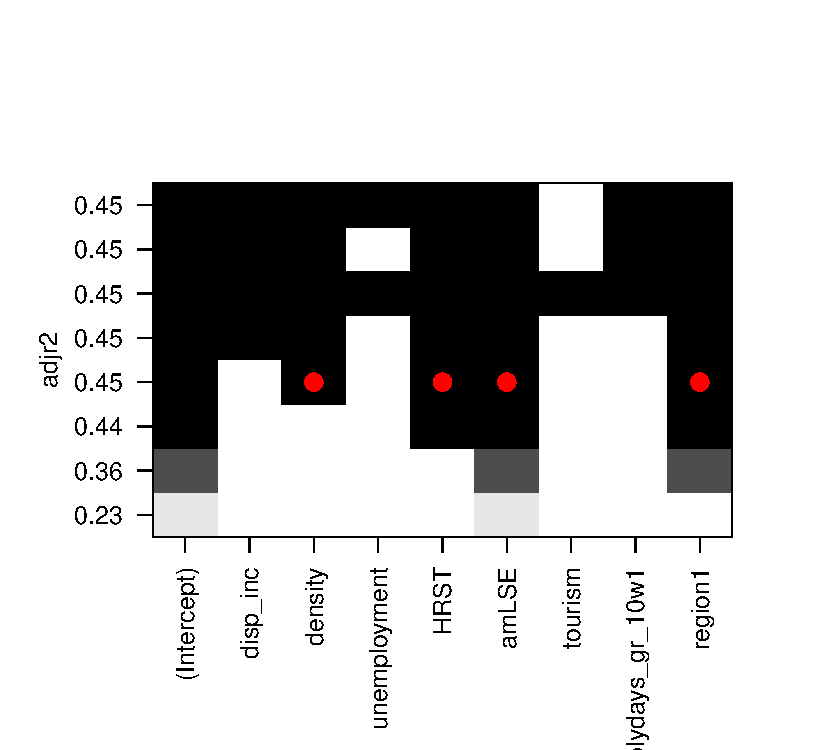
\includegraphics[width=1\textwidth,height=\textheight]{report_files/figure-pdf/best subset-1.pdf}

}

\caption{Adjusted Rsquared Best Subset}

\end{figure}%

\begin{figure}[H]

{\centering 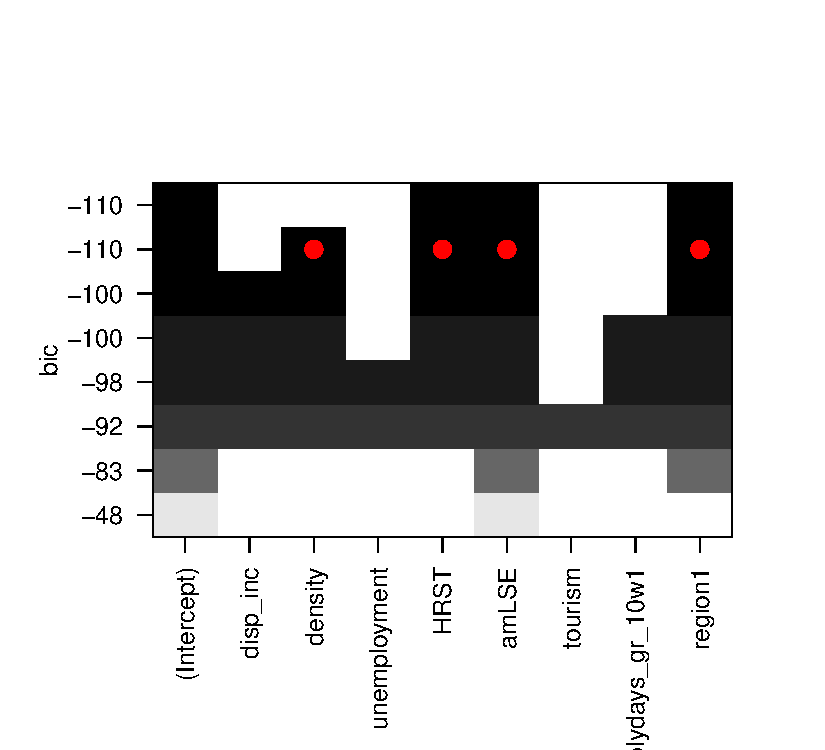
\includegraphics[width=1\textwidth,height=\textheight]{report_files/figure-pdf/bic-1.pdf}

}

\caption{BIC Best Subset}

\end{figure}%

The new linear regression model with selected variables is specified as
follows: \[
\text{Early School Leavers} = \beta_0 + \beta_1 \text{Population Density} + \beta_2\text{Human Resources in Science and Technology} + \]
\[+ \beta_3 \text{Over 25 with at most Lower Secondary Education}+\beta_4 \text {Southern Europe} + \epsilon{_i} \]

The intercept is 11.29, indicating the baseline value of ESL when all
predictors are zero (which is the mean among all the regions as we
centered the covariates). The coefficient for density is 0.06, which is
significant at the 5\% level. This suggests a positive relationship,
where an increase in density is associated with a slight increase in
ESL. The coefficient for amLSE is 0.28 and is highly significant, just
as HRST, which has a coefficient of -0.15, suggesting a strong negative
relationship though. The Southern Region dummy variable shows a large
negative coefficient of -5.63, even if the southern countries of EU
result in a higher ESL rate.

The model has an adjusted R-squared is 0.4463, which is not that small
comparing to the ones of the models we fitted with all the available
variables.

\global\setlength{\Oldarrayrulewidth}{\arrayrulewidth}

\global\setlength{\Oldtabcolsep}{\tabcolsep}

\setlength{\tabcolsep}{2pt}

\renewcommand*{\arraystretch}{1.5}



\providecommand{\ascline}[3]{\noalign{\global\arrayrulewidth #1}\arrayrulecolor[HTML]{#2}\cline{#3}}

\begin{longtable*}[c]{|p{0.98in}|p{0.88in}|p{1.29in}|p{0.75in}|p{0.75in}|p{0.40in}}



\ascline{1.5pt}{666666}{1-6}

\multicolumn{1}{>{\raggedright}m{\dimexpr 0.98in+0\tabcolsep}}{\textcolor[HTML]{000000}{\fontsize{11}{11}\selectfont{\global\setmainfont{Arial}{}}}} & \multicolumn{1}{>{\raggedleft}m{\dimexpr 0.88in+0\tabcolsep}}{\textcolor[HTML]{000000}{\fontsize{11}{11}\selectfont{\global\setmainfont{Arial}{Estimate}}}} & \multicolumn{1}{>{\raggedleft}m{\dimexpr 1.29in+0\tabcolsep}}{\textcolor[HTML]{000000}{\fontsize{11}{11}\selectfont{\global\setmainfont{Arial}{Standard\ Error}}}} & \multicolumn{1}{>{\raggedleft}m{\dimexpr 0.75in+0\tabcolsep}}{\textcolor[HTML]{000000}{\fontsize{11}{11}\selectfont{\global\setmainfont{Arial}{t\ value}}}} & \multicolumn{1}{>{\raggedleft}m{\dimexpr 0.75in+0\tabcolsep}}{\textcolor[HTML]{000000}{\fontsize{11}{11}\selectfont{\global\setmainfont{Arial}{Pr(>|t|)}}}} & \multicolumn{1}{>{\raggedright}m{\dimexpr 0.4in+0\tabcolsep}}{\textcolor[HTML]{000000}{\fontsize{11}{11}\selectfont{\global\setmainfont{Arial}{}}}} \\

\ascline{1.5pt}{666666}{1-6}\endfirsthead 

\ascline{1.5pt}{666666}{1-6}

\multicolumn{1}{>{\raggedright}m{\dimexpr 0.98in+0\tabcolsep}}{\textcolor[HTML]{000000}{\fontsize{11}{11}\selectfont{\global\setmainfont{Arial}{}}}} & \multicolumn{1}{>{\raggedleft}m{\dimexpr 0.88in+0\tabcolsep}}{\textcolor[HTML]{000000}{\fontsize{11}{11}\selectfont{\global\setmainfont{Arial}{Estimate}}}} & \multicolumn{1}{>{\raggedleft}m{\dimexpr 1.29in+0\tabcolsep}}{\textcolor[HTML]{000000}{\fontsize{11}{11}\selectfont{\global\setmainfont{Arial}{Standard\ Error}}}} & \multicolumn{1}{>{\raggedleft}m{\dimexpr 0.75in+0\tabcolsep}}{\textcolor[HTML]{000000}{\fontsize{11}{11}\selectfont{\global\setmainfont{Arial}{t\ value}}}} & \multicolumn{1}{>{\raggedleft}m{\dimexpr 0.75in+0\tabcolsep}}{\textcolor[HTML]{000000}{\fontsize{11}{11}\selectfont{\global\setmainfont{Arial}{Pr(>|t|)}}}} & \multicolumn{1}{>{\raggedright}m{\dimexpr 0.4in+0\tabcolsep}}{\textcolor[HTML]{000000}{\fontsize{11}{11}\selectfont{\global\setmainfont{Arial}{}}}} \\

\ascline{1.5pt}{666666}{1-6}\endhead



\multicolumn{1}{>{\raggedright}m{\dimexpr 0.98in+0\tabcolsep}}{\textcolor[HTML]{000000}{\fontsize{11}{11}\selectfont{\global\setmainfont{Arial}{(Intercept)}}}} & \multicolumn{1}{>{\raggedleft}m{\dimexpr 0.88in+0\tabcolsep}}{\textcolor[HTML]{000000}{\fontsize{11}{11}\selectfont{\global\setmainfont{Arial}{11.292}}}} & \multicolumn{1}{>{\raggedleft}m{\dimexpr 1.29in+0\tabcolsep}}{\textcolor[HTML]{000000}{\fontsize{11}{11}\selectfont{\global\setmainfont{Arial}{0.288}}}} & \multicolumn{1}{>{\raggedleft}m{\dimexpr 0.75in+0\tabcolsep}}{\textcolor[HTML]{000000}{\fontsize{11}{11}\selectfont{\global\setmainfont{Arial}{39.163}}}} & \multicolumn{1}{>{\raggedleft}m{\dimexpr 0.75in+0\tabcolsep}}{\textcolor[HTML]{000000}{\fontsize{11}{11}\selectfont{\global\setmainfont{Arial}{0.0000}}}} & \multicolumn{1}{>{\raggedright}m{\dimexpr 0.4in+0\tabcolsep}}{\textcolor[HTML]{000000}{\fontsize{11}{11}\selectfont{\global\setmainfont{Arial}{***}}}} \\





\multicolumn{1}{>{\raggedright}m{\dimexpr 0.98in+0\tabcolsep}}{\textcolor[HTML]{000000}{\fontsize{11}{11}\selectfont{\global\setmainfont{Arial}{density}}}} & \multicolumn{1}{>{\raggedleft}m{\dimexpr 0.88in+0\tabcolsep}}{\textcolor[HTML]{000000}{\fontsize{11}{11}\selectfont{\global\setmainfont{Arial}{0.060}}}} & \multicolumn{1}{>{\raggedleft}m{\dimexpr 1.29in+0\tabcolsep}}{\textcolor[HTML]{000000}{\fontsize{11}{11}\selectfont{\global\setmainfont{Arial}{0.026}}}} & \multicolumn{1}{>{\raggedleft}m{\dimexpr 0.75in+0\tabcolsep}}{\textcolor[HTML]{000000}{\fontsize{11}{11}\selectfont{\global\setmainfont{Arial}{2.294}}}} & \multicolumn{1}{>{\raggedleft}m{\dimexpr 0.75in+0\tabcolsep}}{\textcolor[HTML]{000000}{\fontsize{11}{11}\selectfont{\global\setmainfont{Arial}{0.0228}}}} & \multicolumn{1}{>{\raggedright}m{\dimexpr 0.4in+0\tabcolsep}}{\textcolor[HTML]{000000}{\fontsize{11}{11}\selectfont{\global\setmainfont{Arial}{\ \ *}}}} \\





\multicolumn{1}{>{\raggedright}m{\dimexpr 0.98in+0\tabcolsep}}{\textcolor[HTML]{000000}{\fontsize{11}{11}\selectfont{\global\setmainfont{Arial}{amLSE}}}} & \multicolumn{1}{>{\raggedleft}m{\dimexpr 0.88in+0\tabcolsep}}{\textcolor[HTML]{000000}{\fontsize{11}{11}\selectfont{\global\setmainfont{Arial}{0.286}}}} & \multicolumn{1}{>{\raggedleft}m{\dimexpr 1.29in+0\tabcolsep}}{\textcolor[HTML]{000000}{\fontsize{11}{11}\selectfont{\global\setmainfont{Arial}{0.031}}}} & \multicolumn{1}{>{\raggedleft}m{\dimexpr 0.75in+0\tabcolsep}}{\textcolor[HTML]{000000}{\fontsize{11}{11}\selectfont{\global\setmainfont{Arial}{9.216}}}} & \multicolumn{1}{>{\raggedleft}m{\dimexpr 0.75in+0\tabcolsep}}{\textcolor[HTML]{000000}{\fontsize{11}{11}\selectfont{\global\setmainfont{Arial}{0.0000}}}} & \multicolumn{1}{>{\raggedright}m{\dimexpr 0.4in+0\tabcolsep}}{\textcolor[HTML]{000000}{\fontsize{11}{11}\selectfont{\global\setmainfont{Arial}{***}}}} \\





\multicolumn{1}{>{\raggedright}m{\dimexpr 0.98in+0\tabcolsep}}{\textcolor[HTML]{000000}{\fontsize{11}{11}\selectfont{\global\setmainfont{Arial}{HRST}}}} & \multicolumn{1}{>{\raggedleft}m{\dimexpr 0.88in+0\tabcolsep}}{\textcolor[HTML]{000000}{\fontsize{11}{11}\selectfont{\global\setmainfont{Arial}{-0.154}}}} & \multicolumn{1}{>{\raggedleft}m{\dimexpr 1.29in+0\tabcolsep}}{\textcolor[HTML]{000000}{\fontsize{11}{11}\selectfont{\global\setmainfont{Arial}{0.025}}}} & \multicolumn{1}{>{\raggedleft}m{\dimexpr 0.75in+0\tabcolsep}}{\textcolor[HTML]{000000}{\fontsize{11}{11}\selectfont{\global\setmainfont{Arial}{-6.133}}}} & \multicolumn{1}{>{\raggedleft}m{\dimexpr 0.75in+0\tabcolsep}}{\textcolor[HTML]{000000}{\fontsize{11}{11}\selectfont{\global\setmainfont{Arial}{0.0000}}}} & \multicolumn{1}{>{\raggedright}m{\dimexpr 0.4in+0\tabcolsep}}{\textcolor[HTML]{000000}{\fontsize{11}{11}\selectfont{\global\setmainfont{Arial}{***}}}} \\





\multicolumn{1}{>{\raggedright}m{\dimexpr 0.98in+0\tabcolsep}}{\textcolor[HTML]{000000}{\fontsize{11}{11}\selectfont{\global\setmainfont{Arial}{region1}}}} & \multicolumn{1}{>{\raggedleft}m{\dimexpr 0.88in+0\tabcolsep}}{\textcolor[HTML]{000000}{\fontsize{11}{11}\selectfont{\global\setmainfont{Arial}{-5.632}}}} & \multicolumn{1}{>{\raggedleft}m{\dimexpr 1.29in+0\tabcolsep}}{\textcolor[HTML]{000000}{\fontsize{11}{11}\selectfont{\global\setmainfont{Arial}{0.768}}}} & \multicolumn{1}{>{\raggedleft}m{\dimexpr 0.75in+0\tabcolsep}}{\textcolor[HTML]{000000}{\fontsize{11}{11}\selectfont{\global\setmainfont{Arial}{-7.331}}}} & \multicolumn{1}{>{\raggedleft}m{\dimexpr 0.75in+0\tabcolsep}}{\textcolor[HTML]{000000}{\fontsize{11}{11}\selectfont{\global\setmainfont{Arial}{0.0000}}}} & \multicolumn{1}{>{\raggedright}m{\dimexpr 0.4in+0\tabcolsep}}{\textcolor[HTML]{000000}{\fontsize{11}{11}\selectfont{\global\setmainfont{Arial}{***}}}} \\

\ascline{1.5pt}{666666}{1-6}



\multicolumn{6}{>{\raggedleft}m{\dimexpr 5.05in+10\tabcolsep}}{\textcolor[HTML]{000000}{\fontsize{11}{11}\selectfont{\global\setmainfont{Arial}{\textit{Signif.\ codes:\ 0\ <=\ '***'\ <\ 0.001\ <\ '**'\ <\ 0.01\ <\ '*'\ <\ 0.05}}}}} \\





\multicolumn{6}{>{\raggedright}m{\dimexpr 5.05in+10\tabcolsep}}{\textcolor[HTML]{000000}{\fontsize{11}{11}\selectfont{\global\setmainfont{Arial}{}}}} \\





\multicolumn{6}{>{\raggedright}m{\dimexpr 5.05in+10\tabcolsep}}{\textcolor[HTML]{000000}{\fontsize{11}{11}\selectfont{\global\setmainfont{Arial}{Residual\ standard\ error:\ 3.271\ on\ 217\ degrees\ of\ freedom}}}} \\





\multicolumn{6}{>{\raggedright}m{\dimexpr 5.05in+10\tabcolsep}}{\textcolor[HTML]{000000}{\fontsize{11}{11}\selectfont{\global\setmainfont{Arial}{Multiple\ R-squared:\ 0.4563,\ Adjusted\ R-squared:\ 0.4463}}}} \\





\multicolumn{6}{>{\raggedright}m{\dimexpr 5.05in+10\tabcolsep}}{\textcolor[HTML]{000000}{\fontsize{11}{11}\selectfont{\global\setmainfont{Arial}{F-statistic:\ 45.53\ on\ 217\ and\ 4\ DF,\ p-value:\ 0.0000}}}} \\





\end{longtable*}



\arrayrulecolor[HTML]{000000}

\global\setlength{\arrayrulewidth}{\Oldarrayrulewidth}

\global\setlength{\tabcolsep}{\Oldtabcolsep}

\renewcommand*{\arraystretch}{1}

There are no outliers or leverage points in this restricted model
either.

\begin{figure}[H]

{\centering 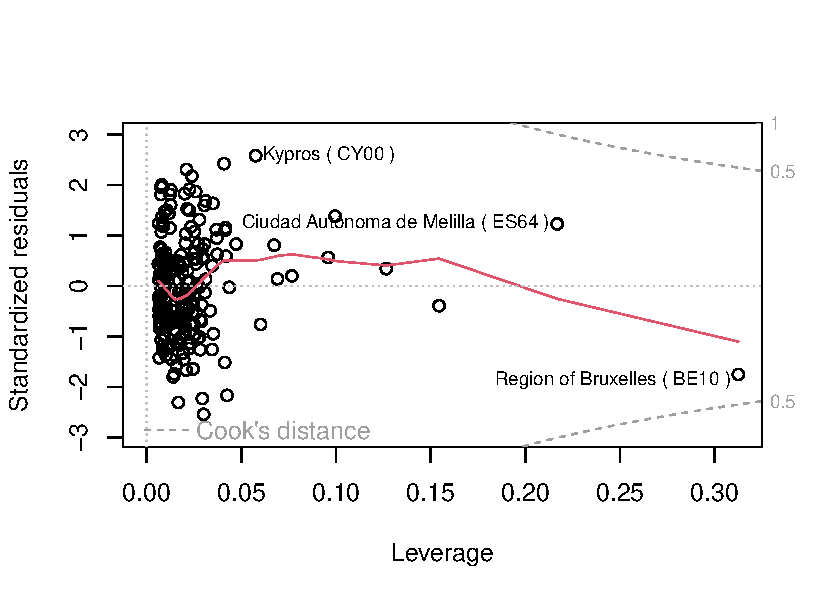
\includegraphics[width=1\textwidth,height=\textheight]{report_files/figure-pdf/residualsvsleverage_sel-1.pdf}

}

\caption{Residuals vs Leverage}

\end{figure}%

The residual diagnostics indicated that the residuals followed a normal
distribution.

\begin{figure}[H]

{\centering 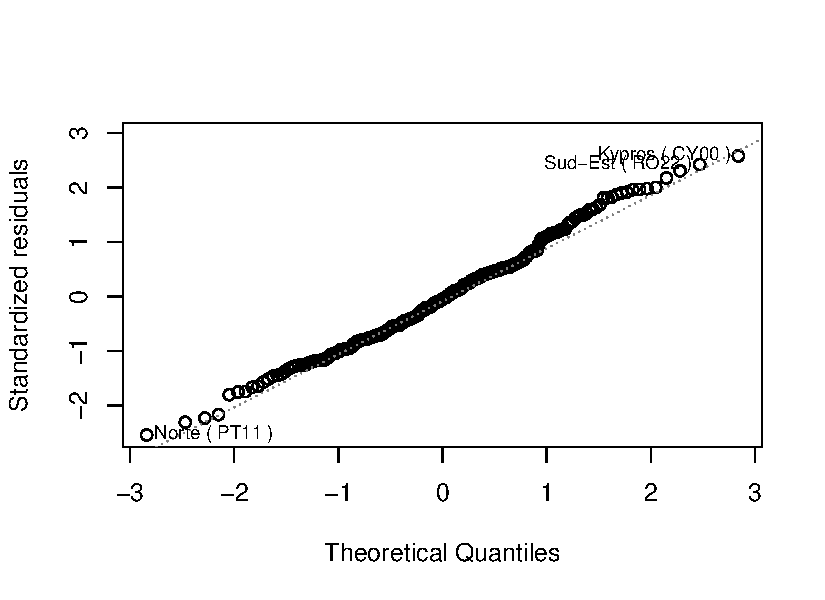
\includegraphics[width=1\textwidth,height=\textheight]{report_files/figure-pdf/qqplot_sel-1.pdf}

}

\caption{QQ-Plot}

\end{figure}%

\begin{figure}[H]

{\centering 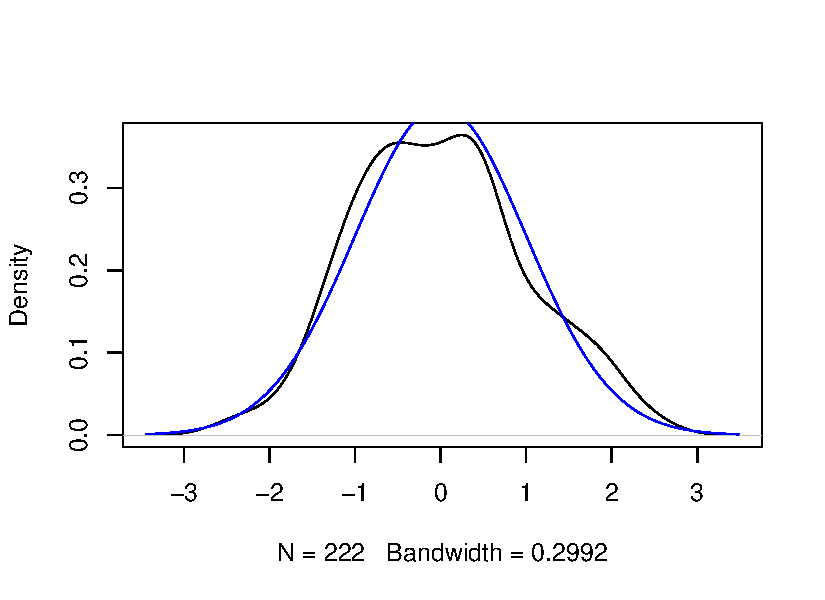
\includegraphics[width=1\textwidth,height=\textheight]{report_files/figure-pdf/normale_sel-1.pdf}

}

\caption{Kernel Hitogram of Residuals}

\end{figure}%

\begin{longtable}[]{@{}rrr@{}}
\caption{Normality Tests of Residuals}\tabularnewline
\toprule\noalign{}
Shapiro-Wilk & Jarque Bera & Kolmogorov-Smirnov \\
\midrule\noalign{}
\endfirsthead
\toprule\noalign{}
Shapiro-Wilk & Jarque Bera & Kolmogorov-Smirnov \\
\midrule\noalign{}
\endhead
\bottomrule\noalign{}
\endlastfoot
0.157 & 0.267 & 0.802 \\
\end{longtable}

To evaluate whether the removal of certain predictors significantly
affects our regression model, we conducted an F-test for nested models.
This test compares the full model, which includes all previous
predictors, with the reduced model with selected variables. The F-test
assesses whether the exclusion of parameters in the reduced model
results in a significant loss of explanatory power. The analysis was
performed comparing the residual sums of squares of the two models. The
resulting p-value indicated that the removal of the predictors did not
significantly diminish the model's fit, suggesting that the reduced
model is preferred due to its simplicity and comparable explanatory
power.

\begin{longtable}[]{@{}lr@{}}
\caption{F-test for Nested Models}\tabularnewline
\toprule\noalign{}
& x \\
\midrule\noalign{}
\endfirsthead
\toprule\noalign{}
& x \\
\midrule\noalign{}
\endhead
\bottomrule\noalign{}
\endlastfoot
RSS of the Reduct Model & 217.000 \\
RSS of the Complete Model & 213.000 \\
p-value & 0.263 \\
\end{longtable}

In the revised model, we addressed the issue of heteroscedasticity
through standard methods without resorting to FGLS.

\begin{figure}[H]

{\centering 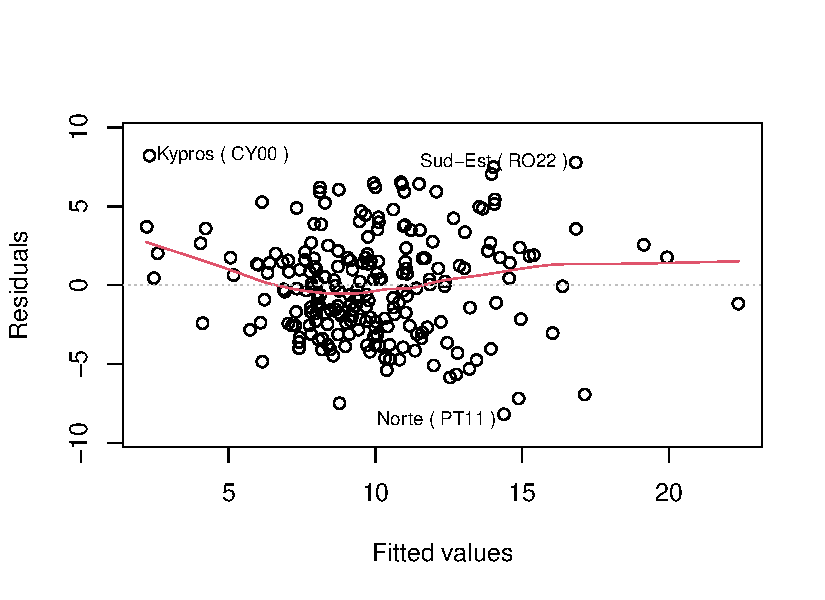
\includegraphics[width=1\textwidth,height=\textheight]{report_files/figure-pdf/residualsvsfitted_sel-1.pdf}

}

\caption{Residuals vs Fitted Values}

\end{figure}%

\begin{longtable}[]{@{}rrr@{}}
\caption{Homoschedasticity Tests of Residuals}\tabularnewline
\toprule\noalign{}
BP.BP & df.df & p-value.BP \\
\midrule\noalign{}
\endfirsthead
\toprule\noalign{}
BP.BP & df.df & p-value.BP \\
\midrule\noalign{}
\endhead
\bottomrule\noalign{}
\endlastfoot
8.948 & 4 & 0.062 \\
\end{longtable}

Despite resolving heteroscedasticity, autocorrelation, particularly
related to the geographical closeness of the observations, remained a
concern. To tackle this issue, we employed a sampled dataset approach
again.

\begin{longtable}[]{@{}rrr@{}}
\caption{Durbin-Watson test}\tabularnewline
\toprule\noalign{}
Autocorrelation & D-W Statistic & p-value \\
\midrule\noalign{}
\endfirsthead
\toprule\noalign{}
Autocorrelation & D-W Statistic & p-value \\
\midrule\noalign{}
\endhead
\bottomrule\noalign{}
\endlastfoot
0.314 & 1.371 & 0 \\
\end{longtable}

\begin{figure}[H]

{\centering 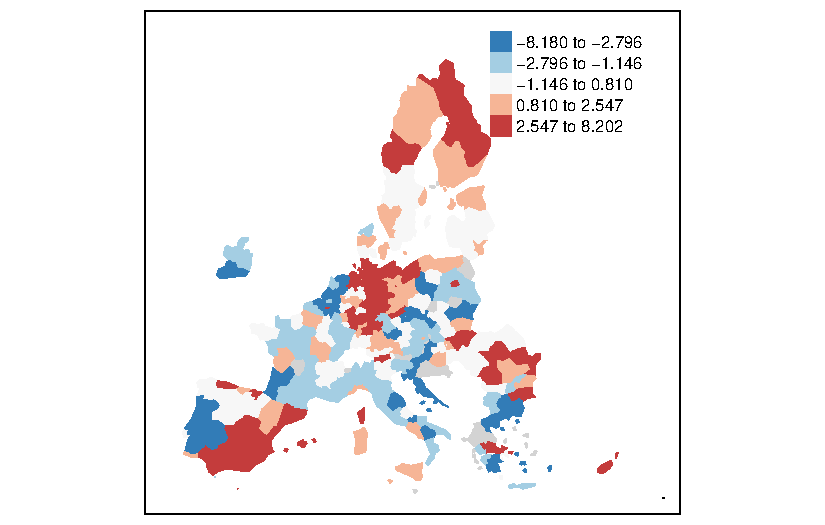
\includegraphics{report_files/figure-pdf/redis_map_sel-1.pdf}

}

\caption{Map of Model's Residuals}

\end{figure}%

In the revised and final model applied to the sampled dataset, the
intercept is 11.22, which represents the expected baseline value of ESL
when all predictors are average and country is not in the southern
region of the EU. The coefficient for density is 0.10, indicating a
significant positive association. Similarly, amLSE has a coefficient of
0.27, reflecting a strong positive impact on ESL. The coefficient for
HRST is -0.10, showing a significant negative relationship just as the
dummy variable Southern Region, which is -5.58.

\global\setlength{\Oldarrayrulewidth}{\arrayrulewidth}

\global\setlength{\Oldtabcolsep}{\tabcolsep}

\setlength{\tabcolsep}{2pt}

\renewcommand*{\arraystretch}{1.5}



\providecommand{\ascline}[3]{\noalign{\global\arrayrulewidth #1}\arrayrulecolor[HTML]{#2}\cline{#3}}

\begin{longtable*}[c]{|p{0.98in}|p{0.88in}|p{1.29in}|p{0.75in}|p{0.75in}|p{0.40in}}



\ascline{1.5pt}{666666}{1-6}

\multicolumn{1}{>{\raggedright}m{\dimexpr 0.98in+0\tabcolsep}}{\textcolor[HTML]{000000}{\fontsize{11}{11}\selectfont{\global\setmainfont{Arial}{}}}} & \multicolumn{1}{>{\raggedleft}m{\dimexpr 0.88in+0\tabcolsep}}{\textcolor[HTML]{000000}{\fontsize{11}{11}\selectfont{\global\setmainfont{Arial}{Estimate}}}} & \multicolumn{1}{>{\raggedleft}m{\dimexpr 1.29in+0\tabcolsep}}{\textcolor[HTML]{000000}{\fontsize{11}{11}\selectfont{\global\setmainfont{Arial}{Standard\ Error}}}} & \multicolumn{1}{>{\raggedleft}m{\dimexpr 0.75in+0\tabcolsep}}{\textcolor[HTML]{000000}{\fontsize{11}{11}\selectfont{\global\setmainfont{Arial}{t\ value}}}} & \multicolumn{1}{>{\raggedleft}m{\dimexpr 0.75in+0\tabcolsep}}{\textcolor[HTML]{000000}{\fontsize{11}{11}\selectfont{\global\setmainfont{Arial}{Pr(>|t|)}}}} & \multicolumn{1}{>{\raggedright}m{\dimexpr 0.4in+0\tabcolsep}}{\textcolor[HTML]{000000}{\fontsize{11}{11}\selectfont{\global\setmainfont{Arial}{}}}} \\

\ascline{1.5pt}{666666}{1-6}\endfirsthead 

\ascline{1.5pt}{666666}{1-6}

\multicolumn{1}{>{\raggedright}m{\dimexpr 0.98in+0\tabcolsep}}{\textcolor[HTML]{000000}{\fontsize{11}{11}\selectfont{\global\setmainfont{Arial}{}}}} & \multicolumn{1}{>{\raggedleft}m{\dimexpr 0.88in+0\tabcolsep}}{\textcolor[HTML]{000000}{\fontsize{11}{11}\selectfont{\global\setmainfont{Arial}{Estimate}}}} & \multicolumn{1}{>{\raggedleft}m{\dimexpr 1.29in+0\tabcolsep}}{\textcolor[HTML]{000000}{\fontsize{11}{11}\selectfont{\global\setmainfont{Arial}{Standard\ Error}}}} & \multicolumn{1}{>{\raggedleft}m{\dimexpr 0.75in+0\tabcolsep}}{\textcolor[HTML]{000000}{\fontsize{11}{11}\selectfont{\global\setmainfont{Arial}{t\ value}}}} & \multicolumn{1}{>{\raggedleft}m{\dimexpr 0.75in+0\tabcolsep}}{\textcolor[HTML]{000000}{\fontsize{11}{11}\selectfont{\global\setmainfont{Arial}{Pr(>|t|)}}}} & \multicolumn{1}{>{\raggedright}m{\dimexpr 0.4in+0\tabcolsep}}{\textcolor[HTML]{000000}{\fontsize{11}{11}\selectfont{\global\setmainfont{Arial}{}}}} \\

\ascline{1.5pt}{666666}{1-6}\endhead



\multicolumn{1}{>{\raggedright}m{\dimexpr 0.98in+0\tabcolsep}}{\textcolor[HTML]{000000}{\fontsize{11}{11}\selectfont{\global\setmainfont{Arial}{(Intercept)}}}} & \multicolumn{1}{>{\raggedleft}m{\dimexpr 0.88in+0\tabcolsep}}{\textcolor[HTML]{000000}{\fontsize{11}{11}\selectfont{\global\setmainfont{Arial}{11.223}}}} & \multicolumn{1}{>{\raggedleft}m{\dimexpr 1.29in+0\tabcolsep}}{\textcolor[HTML]{000000}{\fontsize{11}{11}\selectfont{\global\setmainfont{Arial}{0.443}}}} & \multicolumn{1}{>{\raggedleft}m{\dimexpr 0.75in+0\tabcolsep}}{\textcolor[HTML]{000000}{\fontsize{11}{11}\selectfont{\global\setmainfont{Arial}{25.312}}}} & \multicolumn{1}{>{\raggedleft}m{\dimexpr 0.75in+0\tabcolsep}}{\textcolor[HTML]{000000}{\fontsize{11}{11}\selectfont{\global\setmainfont{Arial}{0.0000}}}} & \multicolumn{1}{>{\raggedright}m{\dimexpr 0.4in+0\tabcolsep}}{\textcolor[HTML]{000000}{\fontsize{11}{11}\selectfont{\global\setmainfont{Arial}{***}}}} \\





\multicolumn{1}{>{\raggedright}m{\dimexpr 0.98in+0\tabcolsep}}{\textcolor[HTML]{000000}{\fontsize{11}{11}\selectfont{\global\setmainfont{Arial}{density}}}} & \multicolumn{1}{>{\raggedleft}m{\dimexpr 0.88in+0\tabcolsep}}{\textcolor[HTML]{000000}{\fontsize{11}{11}\selectfont{\global\setmainfont{Arial}{0.105}}}} & \multicolumn{1}{>{\raggedleft}m{\dimexpr 1.29in+0\tabcolsep}}{\textcolor[HTML]{000000}{\fontsize{11}{11}\selectfont{\global\setmainfont{Arial}{0.040}}}} & \multicolumn{1}{>{\raggedleft}m{\dimexpr 0.75in+0\tabcolsep}}{\textcolor[HTML]{000000}{\fontsize{11}{11}\selectfont{\global\setmainfont{Arial}{2.648}}}} & \multicolumn{1}{>{\raggedleft}m{\dimexpr 0.75in+0\tabcolsep}}{\textcolor[HTML]{000000}{\fontsize{11}{11}\selectfont{\global\setmainfont{Arial}{0.0095}}}} & \multicolumn{1}{>{\raggedright}m{\dimexpr 0.4in+0\tabcolsep}}{\textcolor[HTML]{000000}{\fontsize{11}{11}\selectfont{\global\setmainfont{Arial}{\ **}}}} \\





\multicolumn{1}{>{\raggedright}m{\dimexpr 0.98in+0\tabcolsep}}{\textcolor[HTML]{000000}{\fontsize{11}{11}\selectfont{\global\setmainfont{Arial}{amLSE}}}} & \multicolumn{1}{>{\raggedleft}m{\dimexpr 0.88in+0\tabcolsep}}{\textcolor[HTML]{000000}{\fontsize{11}{11}\selectfont{\global\setmainfont{Arial}{0.272}}}} & \multicolumn{1}{>{\raggedleft}m{\dimexpr 1.29in+0\tabcolsep}}{\textcolor[HTML]{000000}{\fontsize{11}{11}\selectfont{\global\setmainfont{Arial}{0.049}}}} & \multicolumn{1}{>{\raggedleft}m{\dimexpr 0.75in+0\tabcolsep}}{\textcolor[HTML]{000000}{\fontsize{11}{11}\selectfont{\global\setmainfont{Arial}{5.510}}}} & \multicolumn{1}{>{\raggedleft}m{\dimexpr 0.75in+0\tabcolsep}}{\textcolor[HTML]{000000}{\fontsize{11}{11}\selectfont{\global\setmainfont{Arial}{0.0000}}}} & \multicolumn{1}{>{\raggedright}m{\dimexpr 0.4in+0\tabcolsep}}{\textcolor[HTML]{000000}{\fontsize{11}{11}\selectfont{\global\setmainfont{Arial}{***}}}} \\





\multicolumn{1}{>{\raggedright}m{\dimexpr 0.98in+0\tabcolsep}}{\textcolor[HTML]{000000}{\fontsize{11}{11}\selectfont{\global\setmainfont{Arial}{HRST}}}} & \multicolumn{1}{>{\raggedleft}m{\dimexpr 0.88in+0\tabcolsep}}{\textcolor[HTML]{000000}{\fontsize{11}{11}\selectfont{\global\setmainfont{Arial}{-0.109}}}} & \multicolumn{1}{>{\raggedleft}m{\dimexpr 1.29in+0\tabcolsep}}{\textcolor[HTML]{000000}{\fontsize{11}{11}\selectfont{\global\setmainfont{Arial}{0.036}}}} & \multicolumn{1}{>{\raggedleft}m{\dimexpr 0.75in+0\tabcolsep}}{\textcolor[HTML]{000000}{\fontsize{11}{11}\selectfont{\global\setmainfont{Arial}{-2.982}}}} & \multicolumn{1}{>{\raggedleft}m{\dimexpr 0.75in+0\tabcolsep}}{\textcolor[HTML]{000000}{\fontsize{11}{11}\selectfont{\global\setmainfont{Arial}{0.0036}}}} & \multicolumn{1}{>{\raggedright}m{\dimexpr 0.4in+0\tabcolsep}}{\textcolor[HTML]{000000}{\fontsize{11}{11}\selectfont{\global\setmainfont{Arial}{\ **}}}} \\





\multicolumn{1}{>{\raggedright}m{\dimexpr 0.98in+0\tabcolsep}}{\textcolor[HTML]{000000}{\fontsize{11}{11}\selectfont{\global\setmainfont{Arial}{region1}}}} & \multicolumn{1}{>{\raggedleft}m{\dimexpr 0.88in+0\tabcolsep}}{\textcolor[HTML]{000000}{\fontsize{11}{11}\selectfont{\global\setmainfont{Arial}{-5.586}}}} & \multicolumn{1}{>{\raggedleft}m{\dimexpr 1.29in+0\tabcolsep}}{\textcolor[HTML]{000000}{\fontsize{11}{11}\selectfont{\global\setmainfont{Arial}{1.124}}}} & \multicolumn{1}{>{\raggedleft}m{\dimexpr 0.75in+0\tabcolsep}}{\textcolor[HTML]{000000}{\fontsize{11}{11}\selectfont{\global\setmainfont{Arial}{-4.971}}}} & \multicolumn{1}{>{\raggedleft}m{\dimexpr 0.75in+0\tabcolsep}}{\textcolor[HTML]{000000}{\fontsize{11}{11}\selectfont{\global\setmainfont{Arial}{0.0000}}}} & \multicolumn{1}{>{\raggedright}m{\dimexpr 0.4in+0\tabcolsep}}{\textcolor[HTML]{000000}{\fontsize{11}{11}\selectfont{\global\setmainfont{Arial}{***}}}} \\

\ascline{1.5pt}{666666}{1-6}



\multicolumn{6}{>{\raggedleft}m{\dimexpr 5.05in+10\tabcolsep}}{\textcolor[HTML]{000000}{\fontsize{11}{11}\selectfont{\global\setmainfont{Arial}{\textit{Signif.\ codes:\ 0\ <=\ '***'\ <\ 0.001\ <\ '**'\ <\ 0.01\ <\ '*'\ <\ 0.05}}}}} \\





\multicolumn{6}{>{\raggedright}m{\dimexpr 5.05in+10\tabcolsep}}{\textcolor[HTML]{000000}{\fontsize{11}{11}\selectfont{\global\setmainfont{Arial}{}}}} \\





\multicolumn{6}{>{\raggedright}m{\dimexpr 5.05in+10\tabcolsep}}{\textcolor[HTML]{000000}{\fontsize{11}{11}\selectfont{\global\setmainfont{Arial}{Residual\ standard\ error:\ 3.237\ on\ 95\ degrees\ of\ freedom}}}} \\





\multicolumn{6}{>{\raggedright}m{\dimexpr 5.05in+10\tabcolsep}}{\textcolor[HTML]{000000}{\fontsize{11}{11}\selectfont{\global\setmainfont{Arial}{Multiple\ R-squared:\ 0.4605,\ Adjusted\ R-squared:\ 0.4378}}}} \\





\multicolumn{6}{>{\raggedright}m{\dimexpr 5.05in+10\tabcolsep}}{\textcolor[HTML]{000000}{\fontsize{11}{11}\selectfont{\global\setmainfont{Arial}{F-statistic:\ 20.28\ on\ 95\ and\ 4\ DF,\ p-value:\ 0.0000}}}} \\





\end{longtable*}



\arrayrulecolor[HTML]{000000}

\global\setlength{\arrayrulewidth}{\Oldarrayrulewidth}

\global\setlength{\tabcolsep}{\Oldtabcolsep}

\renewcommand*{\arraystretch}{1}

In addition to evaluating the final model's performance, we ran
simulations on various sampled datasets to further assess the robustness
of our results. The Shapiro-Wilk test p-value exceeded 0.05 in 92 out of
100 sampled datasets, indicating that the normality of residuals was
maintained across most samples. Similarly, the Breusch-Pagan test
p-value was greater than 0.05 in 76 out of 100 datasets, suggesting that
heteroscedasticity was not a significant issue in the majority of cases.
The Durbin-Watson test p-value was above 0.05 in 89 out of 100 datasets,
confirming that autocorrelation was not a concern in most instances.
These findings collectively support the reliability of the final model,
demonstrating consistent adherence to the assumptions of normality,
homoscedasticity, and independence across different samples.

\begin{longtable}[]{@{}lr@{}}
\caption{Simulation Results for Diagnostic Tests}\tabularnewline
\toprule\noalign{}
Test & Number.of.Times.p.value\ldots0.05 \\
\midrule\noalign{}
\endfirsthead
\toprule\noalign{}
Test & Number.of.Times.p.value\ldots0.05 \\
\midrule\noalign{}
\endhead
\bottomrule\noalign{}
\endlastfoot
Shapiro-Wilk & 92 \\
Breusch-Pagan & 76 \\
Durbin-Watson & 89 \\
\end{longtable}

Finally, the diagnostic checks confirmed that there were no significant
issues with multicollinearity among the predictors in the models. VIF
values were obviously smaller that the models fitted with all the
variables.

\begin{longtable}[]{@{}lrrrr@{}}
\caption{VIFs of Covariates}\tabularnewline
\toprule\noalign{}
& density & amLSE & HRST & region \\
\midrule\noalign{}
\endfirsthead
\toprule\noalign{}
& density & amLSE & HRST & region \\
\midrule\noalign{}
\endhead
\bottomrule\noalign{}
\endlastfoot
OLS & 1.129 & 2.502 & 1.367 & 2.254 \\
OLS S.D. & 1.262 & 2.497 & 1.572 & 2.484 \\
\end{longtable}

\section{Conclusion}\label{conclusion}

This study provides a comprehensive analysis of the factors influencing
Early School Leaving (ESL) in the European Union, shedding light on the
multifaceted nature of the problem. This analysis reveals that a
combination of demographic, socio-economic, cultural, and educational
factors contribute to the phenomenon of ESL, thereby reinforcing the
critical role of education as a social elevator that promotes
socio-economic mobility and reduces inequality.

The percentage of adults over 25 with at most lower secondary education
(amLSE) emerged as the most significant predictor of ESL, highlighting
the influence of educational attainment within communities. This
underscores the need for targeted educational interventions that not
only support current students but also address the broader educational
environment, including adult education programs.

The negative relationship between HRST and ESL suggests that regions
with a higher proportion of the population engaged in science and
technology exhibit lower rates of ESL. This indicates the importance of
fostering environments that support and encourage careers in science and
technology to reduce dropout rates. Educational policies that emphasize
STEM (Science, Technology, Engineering, and Mathematics) education can
be pivotal in addressing ESL.

The positive association between population density and ESL implies that
more densely populated areas, often urban centers, experience higher
dropout rates. This may be due to a range of urban-specific challenges
such as socio-economic disparities, school quality variations, and other
urban stressors. Educational policies must address urban challenges,
potentially through increased support for schools in densely populated
areas and initiatives that engage students and communities.

Although mean disposable income (MDI) and unemployment were not retained
in the final model, their initial analysis suggested that economic
factors play a role in ESL. While MDI had a statistically significant
relationship with ESL in individual models, the low R-squared values
indicate the presence of other influential factors. This points to the
complex relationship between economic conditions and education,
suggesting that policies aimed at improving economic stability may
indirectly impact ESL rates.

The data reveals that Southern European regions perform worse in ESL
rates compared to other EU regions, even though the Southern Europe
dummy variable shows a negative coefficient. This is due to these
regions' poorer performance in other covariates, such as educational
attainment and HRST, departing far from the average of other countries.
Southern regions have historically faced significant socio-economic
challenges, which are reflected in their higher ESL rates.

\subsubsection*{References}\label{references}
\addcontentsline{toc}{subsubsection}{References}

\phantomsection\label{refs}
\begin{CSLReferences}{1}{0}
\bibitem[\citeproctext]{ref-bitsakos2021causes}
Bitsakos, Nikolaos. 2021. {``CAUSES OF EARLY SCHOOL LEAVING AND
PREVENTION MEASURES: SCHOOL DIRECTORS'INSIGHTS.''} \emph{European
Journal of Education Studies} 8 (5).

\bibitem[\citeproctext]{ref-causesruralarea}
Bosoanca, Bianca. 2021. {``The Causes of School Drop-Out Among Scholars
in Rural Areas.''} \emph{Review of Socio-Economic Perspectives} 6
(202182): 59--65.

\bibitem[\citeproctext]{ref-nowayback}
Byrne, Delma, and Emer Smyth. 2010. {``No Way Back? The Dynamics of
Early School Leaving.''}

\bibitem[\citeproctext]{ref-de2012comparing}
De Witte, Kristof, and Chris Van Klaveren. 2012. {``Comparing Students
by a Matching Analysis--on Early School Leaving in Dutch Cities.''}
\emph{Applied Economics} 44 (28): 3679--90.

\bibitem[\citeproctext]{ref-dispinc}
Eurostat. 2024a. {``Disposable Income of Private Households by NUTS 2
Regions.''} 2024. \url{https://doi.org/10.2908/TGS00026}.

\bibitem[\citeproctext]{ref-eslexpl}
---------. 2024b. {``Early Leavers from Education and Training.''} 2024.
\url{https://ec.europa.eu/eurostat/statistics-explained/index.php?title=Early_leavers_from_education_and_training}.

\bibitem[\citeproctext]{ref-esl}
---------. 2024c. {``Early Leavers from Education and Training by Sex
and NUTS 2 Regions.''} 2024. \url{https://doi.org/10.2908/EDAT_LFSE_16}.

\bibitem[\citeproctext]{ref-HRST}
---------. 2024d. {``Human Resources in Science and Technology (HRST) by
NUTS 2 Regions.''} 2024. \url{https://doi.org/10.2908/tgs00038}.

\bibitem[\citeproctext]{ref-nights}
---------. 2024e. {``Nights Spent at Tourist Accommodation
Establishments by NUTS 2 Regions.''} 2024.
\url{https://doi.org/10.2908/TGS00111}.

\bibitem[\citeproctext]{ref-popbyed}
---------. 2024f. {``Population by Educational Attainment Level, Sex and
NUTS 2 Regions (.''} 2024. \url{https://doi.org/10.2908/edat_lfse_04}.

\bibitem[\citeproctext]{ref-density}
---------. 2024g. {``Population Density by NUTS 2 Region.''} 2024.
\url{https://doi.org/10.2908/TGS00024}.

\bibitem[\citeproctext]{ref-pop}
---------. 2024h. {``Population on 1 January by Age, Sex and NUTS 2
Region.''} 2024. \url{https://doi.org/10.2908/DEMO_R_D2JAN}.

\bibitem[\citeproctext]{ref-unemployment}
---------. 2024i. {``Unemployment Rate by NUTS 2 Regions.''} 2024.
\url{https://doi.org/10.2908/TGS00010}.

\bibitem[\citeproctext]{ref-nutsexpl}
Gouardères, Frédéric. 2024. {``Nomenclatura Comune Delle Unità
Territoriali Statistiche (NUTS).''} 2024.
\url{https://www.europarl.europa.eu/factsheets/it/sheet/99/nomenclatura-comune-delle-unita-territoriali-statistiche-nuts-}.

\bibitem[\citeproctext]{ref-minguez2013early}
Mı́nguez, Almudena Moreno. 2013. {``The Early School Leaving in Europe:
Approaching the Explanatory Factors.''} \emph{New Horizons in Education}
61 (2).

\bibitem[\citeproctext]{ref-unsd}
United\_Nations\_Statistics\_Division. n.d. {``Standard Country or Area
Codes for Statistical Use (M49).''}
\url{https://unstats.un.org/unsd/methodology/m49/}.

\end{CSLReferences}



\end{document}
